\documentclass[12pt]{article}

\usepackage[left=1in,right=1in,top=1in,bottom=1in]{geometry}
\usepackage[english]{babel}
\usepackage{fontspec}
\setmainfont[Mapping=tex-text]{Times New Roman}
\usepackage[colorlinks = true,
linkcolor = black,
urlcolor  = blue,
citecolor = blue,
anchorcolor = blue]{hyperref}
\usepackage[inline] {enumitem}
\usepackage[normalem]{ulem}
\usepackage{soul}
\setul{0.25ex}{}

\usepackage{color, amsmath}
\usepackage{mathtools}
\usepackage{setspace}
\usepackage{lastpage}
\usepackage{fancyhdr}
\usepackage{float}
\usepackage{graphicx}
\usepackage{amsmath}
\usepackage{amsfonts}
\usepackage{amssymb}
\usepackage{subcaption}
\setlength{\parskip}{1em}
\setlength\parindent{0pt}
\pagestyle{fancy}
\fancyhf{}
\chead{Data Set-Sample Control Problems}
\cfoot{Page \thepage\ of \pageref{LastPage}}
\graphicspath{{figures}}

\newcommand{\tp}{T}
\newcommand{\bmtx}{\begin{bmatrix}}
\newcommand{\emtx}{\end{bmatrix}}
\newcommand{\bsmtx}{\left[ \begin{smallmatrix}} 
\newcommand{\esmtx}{\end{smallmatrix} \right]} 
\newcommand{\bmatarray}[1]{\left[\begin{array}{#1}}
\newcommand{\ematarray}{\end{array}\right]} 

\newcommand{\bmat}[1]{\begin{bmatrix} #1 \end{bmatrix}}
\newcommand{\pmat}[1]{\begin{pmatrix} #1 \end{pmatrix}}

\usepackage{graphicx} % For \resizebox
\usepackage{amssymb}  % For \times and \checkmark
\usepackage{tikz}

% Define a new command for the combined checkmark and times symbol
\newcommand{\halfcheck}{
\tikz[scale=0.6,baseline=-0.5ex]{
    % Draw checkmark
    \draw[line width=0.8pt] (0,0.2) -- (0.2,0) -- (0.6,0.4);
    % Draw times
    \draw[line width=0.8pt] (0.2,0.4) -- (0.6,0);

}%
}


\begin{document}
In our evaluation process, a control engineer expert carefully assesses the answers generated by GPT or other Large Language Models (LLMs). For each question, if the final answer aligns with the correct solution, it is considered correct. In some cases, while the reasoning steps may not be entirely correct, if the final answer is accurate and doesn't compromise the overall solution, it is still regarded as correct. For the problems in which the final answer is not correct, the type of error is categorized as follows:
\begin{itemize}
    \item \textbf{Calculation Complexity:} The mathematical computation was overly intricate, requiring more information from the user.
    \item \textbf{Calculation Error:} This denotes that mistakes were made during the mathematical computation in the process of solving the problem.
    \item \textbf{Reasoning Error:} This refers to a flaw in the logical progression or inference made while solving the problem.
    \item \textbf{Incorrect Knowledge:} This means that the answer was based on incorrect information or understanding of the problem.
    \item \textbf{Lack of Knowledge:} The solution was hindered by a lack of understanding or familiarity with the relevant concepts.
    \item \textbf{Misreading The Plot:} This refers to problems in which it is necessary to extract data from the provided plots in the statement of the problem, but LLMs could not correctly extract the graphical data.
    \item \textbf{Didn't solve:} The problem was left unsolved mainly by providing a general approach; however, no mathematical approaches are provided.
\end{itemize}

In the process of presenting problems to LLMs, we employed the following statement, which was provided alongside the problem statement, to generate the results.\\
\textit{"Provide a concise yet comprehensive response to the following question, including a confidence level ranging from 0 to 100 for the accuracy of the answer. Additionally, include the LaTeX code for the entire response, encompassing both the answer and the confidence score."}\\
\clearpage
Listed below are the comprehensive topics from which we have extracted questions, covering various aspects of control theory, to compile our dataset.

\textbf{Table of Contents:}
\begin{enumerate}
    \item Differential Equations, Laplace Transform and Preliminaries
    \item Stability
    \item Time Response of Dynamical Systems
    \item Block Diagrams
    \item Control System Design
    \item Bode Analysis
    \item Root-Locus Design
    \item Nyquist Design
    \item Gain/Phase Margins
    \item Advanced Topics (Lyapunov Stability, Controllability and Observability)
    \item System Sensitivity Measures
    \item Loop-Shaping
\end{enumerate}

\clearpage

\section{Differential Equations, Laplace Transform and Preliminaries}
\subsection{Differential Equations}
Determine the transfer function of a linear time invariant (LTI) system given the following information:
\begin{enumerate}
    \item The system has relative degree 3.
    \item It has 3 poles, of which 2 are at -2 and -4.
    \item The impulse response resembles a step response for a stable linear system with a steady state value of 0.25.
\end{enumerate}


\textbf{\textcolor{red}{Solution :}} \\
% Short Answer: G(s) = \frac{2}{s(s + 2)(s + 4)}
% Reasoning Steps:
Given a linear time-invariant (LTI) system with specific characteristics, we aim to determine its transfer function. The details and solution steps are as follows:

\textbf{System Characteristics}
\begin{itemize}
    \item The system has a relative degree 3 with 3 poles, hence it has no finite zeros.
    \item It has 3 poles, hence it takes the form:
    \begin{equation}
    G(s) = \frac{K}{A(s)(s + 2)(s + 4)}
    \end{equation}
    \item Since the impulse response resembles a step response with a steady state value, we conclude the system must contain a pole at zero. Therefore, the transfer function is of the form:
    \begin{equation}
    G(s) = \frac{K}{s(s + 2)(s + 4)}
    \end{equation}
\end{itemize}

\textbf{Determination of \(K\)}

Using the final value theorem to determine \(K\), we have:
\begin{align}
\lim_{s \to 0} G(s) &= \lim_{s \to 0} \frac{sK}{s(s + 2)(s + 4)} \\
&= \frac{K}{8}
\end{align}
Given the steady state value of 0.25, i.e., \(\lim_{s \to 0} sG(s) = 0.25\), we find \(K = 2\).
Therefore, the transfer function of the system is:
\begin{equation}
G(s) = \frac{2}{s(s + 2)(s + 4)}
\end{equation}
% Problem End

\clearpage
\subsection{Initial Value Theorem}

Consider a system with the transfer function given by
\begin{equation}
H(s) = \frac{2(s + 1)}{s^2 + 4s + 9}
\end{equation}
and denote by \(g(t)\) the unit step response with zero initial conditions. Compute the initial slope of \(g(t)\), i.e., the slope at \(t = 0+\).

\textbf{\textcolor{red}{Solution :}} \\
% Short Answer: 2
% Reasoning Steps:
We first note that the derivative of \(g(t)\) is the response to the derivative of the unit step, i.e., it is equal to the response to a Dirac delta. Hence, we have
\begin{equation}
\mathcal{L}\left\{ \frac{dg(t)}{dt} \right\} = \mathcal{L}\{h(t)\} = H(s)
\end{equation}
Therefore, the answer to the question translates into computing \(h(0+)\). This can be computed via the Initial Value Theorem. This yields
\begin{equation}
\dot{g}(0+) = h(0+) = \lim_{s \to \infty} sH(s) = \lim_{s \to \infty} \frac{2s(s + 1)}{s^2 + 4s + 9} = 2
\end{equation}
% Problem End

\clearpage

\subsection{Undershoot}

Consider a system with a transfer function given by
\begin{equation}
H(s) = \frac{2}{s + 1} + \frac{\alpha}{s + 2}
\end{equation}
where \(\alpha\) is a real number. Is there a range of real values for \(\alpha\) such that the system's unit step response exhibits undershoot? 


\textbf{\textcolor{red}{Solution :}} \\
% Short Answer: [-4,-2]
% Reasoning Steps:
We first note that if \(\alpha > 0\), the unit step response is always positive, thus no undershoot occurs. 

To have undershoot in the unit step response, it is sufficient that a linear system have a real zero in the open Right Half Plane (RHP) -- a Non-Minimum Phase (NMP) zero. To investigate that possibility, we add the two fractions in \(H(s)\) to yield:
\begin{equation}
H(s) = \frac{2s + 4 + \alpha s + \alpha}{(s + 1)(s + 2)} = (4+\alpha)\frac{\frac{2 + \alpha}{4 + \alpha}s + 1}{(s + 1)(s + 2)}
\end{equation}

Then, we have a NMP zero if and only if \(-4 < \alpha < -2\).
% Problem End 
\clearpage

\subsection{Superposition Principle}

Consider a linear system with transfer function \(G(s) = \frac{4}{s+2}\). Let \(u\) denote the input and \(y\) denote the output. The response of \(G(s)\) with \(u(t) = 2\) for \(t \geq 0\), \(u(t) = 0\) for \(t < 0\), and zero initial conditions is \(y(t) = 4(1 - e^{-2t})\).

\begin{enumerate}
    \item[(a)] What is the response \(y_A\) from zero initial conditions if \(u_A(t) = -1\) for \(t \geq 0\)? Provide your answer as an explicit function of \(y(t)\).
    \item[(b)] Analyze the response \(y_B(t)\) from zero initial conditions for a piecewise input:
    \[ u_B(t) = 
    \begin{cases} 
    2 & 0 \leq t < 10, \\
    4 & t \geq 10.
    \end{cases}
    \]
    Express \(y_B(t)\) as a mathematical expression in terms of \(y(t)\), using the principle of superposition and time-invariance.
\end{enumerate}

\textbf{\textcolor{red}{Solution :}} \\
% Short Answer: - \textbf{For part (a):} "The response \(y_A(t) =  -\frac{1}{2}y(t)\)." \\- \textbf{For part (b):} "The response \(y_B(t) =  y(t) + y(t - 10)\)."
% Reasoning Steps:
\begin{enumerate}
    \item[(a)] Note that \(u_A = -\frac{1}{2}u\). By the principle of superposition (scaling), the response due to \(u_A\) is
    \[y_A = -\frac{1}{2}y = -2(1 - e^{-2t}).\]
    
    \item[(b)] Note that \(u_B(t) = u(t) + u(t - 10)\) where \(u(t - 10)\) is the original input shifted by 10 sec. By time-invariance, the response due to \(u(t - 10)\) is given by \(y(t - 10)\). By the principle of superposition (addition), the response due to \(u_B\) is given by \(y_B(t) = y(t) + y(t - 10)\). This plot is shown below.

\end{enumerate}


\begin{figure}[H]
    \centering
    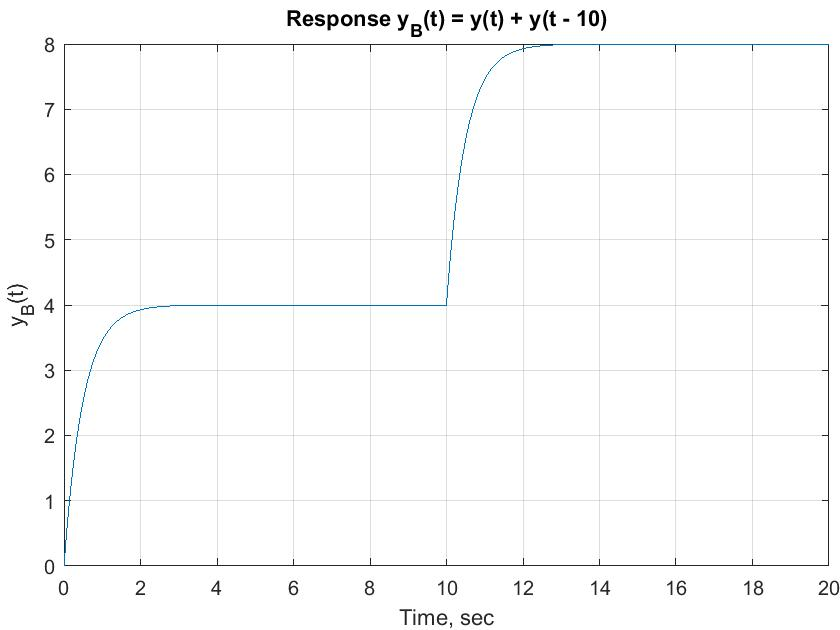
\includegraphics[width=0.5\textwidth]{figs/1.4.jpg}
    \caption{The system response \(y_B(t)\) over time.}
    \label{fig:yb}
\end{figure}
% Problem End


\clearpage
\subsection{Ordinary Differential Equation Representation of Transfer Functions}

Consider two systems \(G_1(s) = \frac{-3}{s+11}\) and \(G_2(s) = \frac{2}{s+9}\).

\begin{enumerate}
    \item[(a)] What is the ODE that represents the serial interconnection \(H(s) = G_2(s)G_1(s)\)?

    \item[(b)] What is the ODE that represents the parallel interconnection \(H(s) = G_1(s) + G_2(s)\)?
\end{enumerate}

\textbf{\textcolor{red}{Solution :}} 
% Short Answer: - \textbf{For part (a):} "\(\ddot{y}(t) + 20\dot{y}(t) + 99y(t) = -6u(t)\)" \\- \textbf{For part (b):} "\(\ddot{y}(t) + 20\dot{y}(t) + 99y(t) = -\dot{u}(t) - 5u(t)\)."
% Reasoning Steps:
\begin{enumerate}
    \item[(a)] Multiplication of the transfer functions yields:

    \begin{equation}
    H(s) = \frac{2}{s + 9} \times \left(\frac{-3}{s + 11}\right) = \frac{-6}{s^2 + 20s + 99}
    \end{equation}
    The corresponding ODE from input \(u\) to output \(y\) is:
    \begin{equation}
    \ddot{y}(t) + 20\dot{y}(t) + 99y(t) = -6u(t)
    \end{equation}
    

    \item[(b)] Addition of the transfer functions yields:


    \begin{equation}
    H(s) = \frac{-3}{s + 11} + \frac{2}{s + 9} = \frac{-3(s + 9) + 2(s + 11)}{(s + 11)(s + 9)} = \frac{-s - 5}{s^2 + 20s + 99}
    \end{equation}
    The corresponding ODE from input \(u\) to output \(y\) is:
    \begin{equation}
    \ddot{y}(t) + 20\dot{y}(t) + 99y(t) = -\dot{u}(t) - 5u(t)
    \end{equation}
\end{enumerate}
% Problem End

\clearpage

\subsection{Proportional Controller}

Consider the following first order system:
\begin{equation}
\dot{y} = -0.5y + 2u; \quad y(0) = 0
\end{equation}
Consider a proportional control law \(u(t) = K_p(r(t) - y(t))\) where \(r(t)\) is the reference command. Consider a unit step command:

    \[ r(t) =
    \begin{cases} 
    0 & \text{for } t < 0 \text{ sec} \\
    1 & \text{for } t \geq 0 \text{ sec}
    \end{cases}
    \quad (2)
    \]
For what gains \(K_p\) is \(\lvert u(t) \rvert \leq 1\) for all time?
Please format your answer as follows: 
If there is a specific range, answer with 'Range: [lower bound, upper bound]'.
If there is no range that satisfies the condition, answer with 'No valid range'.
If there is a specific value, answer with 'Value: [value]'."

\textbf{\textcolor{red}{Solution :}} \\
% Short Answer: Range: [-0.2, 1]
% Reasoning Steps:
First, note that we must ensure that the closed-loop is stable otherwise the control will grow unbounded. The closed-loop is modeled by:
\begin{equation}
\dot{y}(t) + (0.5 + 2K_p)y(t) = 2K_pr(t)
\end{equation}
Thus, \(K_p > -0.25\) is required for stability. There are two cases to consider: (i) \(K_p \geq 0\) and (ii) \(-0.25 < K_p < 0\).

First consider the case \(K_p \geq 0\). In this case, the output starts at \(y(0) = 0\) and converges exponentially to the final value \(\bar{y} = \frac{2K_p}{0.5+2K_p}\). The error \(e(t) = r(t) - y(t)\) thus starts at \(e(0) = 1\) and converges to the following final value:
\begin{equation}
\bar{e} = 1 - \frac{2K_p}{0.5 + 2K_p} = \frac{0.5}{0.5 + 2K_p} \leq 1
\end{equation}
In other words, \(e\) achieves its largest value at \(t = 0\) and decays to a smaller value. Thus the control effort \(u(t) = K_pe(t)\) achieves its largest value at \(t = 0\). To ensure \(|u(t)| \leq 1\) it is sufficient to require \(u(0) = K_pe(0) = K_p \leq 1\).

The alternative case \(-0.25 < K_p < 0\) actually causes the error to grow from \(e(0) = 1\) to its final value. In this case, the controller is acting to degrade tracking, which would not be typical. The hint given in the problem statement is incorrect for this case. It is fine if you only considered positive gains. However, to analyze this case you can use the expression above for the final value \(\bar{e}\). Use this expression to show that \(K_p \geq -0.2\) is required to ensure \(|u(t)| \leq 1\).

Combining these results, the input satisfies \(|u(t)| \leq 1\) for all time if the gain is selected in the range \(-0.2 \leq K_p \leq 1\).

% Problem End
\clearpage
\subsection{Equilibrium}

Consider the scalar ODE
\begin{equation}
    \dot{x} = x^2-1
\end{equation}
\begin{enumerate}
    \item[(a)] Find all the equilibria
    \item[(b)] Compute the linearization of the ODE about each equilibrium and determine the stability.
\end{enumerate}

\textbf{\textcolor{red}{Solution :}}
%Short Answer: Equilibria: [-1,1]. "At $x = 1$, the equilibrium is unstable because the derivative $f'(x) = 2$ is positive." "At $x = -1$, the equilibrium is stable because the derivative $f'(x) = -2$ is negative."
% Reasoning Steps:
\begin{enumerate}
\item[(a)] 


The equilibria occur where $\dot{x} = 0$. Solving the equation $x^2 - 1 = 0$, we find the equilibrium points are $x = 1$ and $x = -1$.

\item[(b)] 


The linearization involves computing the derivative of $f(x) = x^2 - 1$ with respect to $x$, which is $f'(x) = 2x$. Evaluating this derivative at each equilibrium point:

\begin{itemize}
    \item For $x = 1$, $f'(1) = 2$. Since $f'(1) > 0$, the equilibrium at $x = 1$ is unstable.
    \item For $x = -1$, $f'(-1) = -2$. Since $f'(-1) < 0$, the equilibrium at $x = -1$ is stable.
\end{itemize}
Thus, the equilibrium at $x = 1$ is unstable, while the equilibrium at $x = -1$ is stable.

\end{enumerate}
% Problem End

\clearpage
\subsection{State-Space Representation of an ODE}


Consider the triple integrator:
\begin{equation}
    \frac{d^3y}{dt^3} = u
\end{equation}
\begin{enumerate}
    \item[(a)] Obtain a state-space representation of the form \(\dot{x} = Ax + Bu\) for this system.

    \item[(b)] Compute \(e^{At}\) and use it to obtain the solution with \(y(0) = \dot{y}(0) = \ddot{y}(0) = 1\) and \(u(t) = 0\)
\end{enumerate}


\textbf{\textcolor{red}{Solution :}}
% Short Answer: - \textbf{For part (a):} "State-space representation is given by matrices \(A = \begin{bmatrix} 0 & 1 & 0 \\ 0 & 0 & 1 \\ 0 & 0 & 0 \end{bmatrix}\) and \(B = \begin{bmatrix} 0 \\ 0 \\ 1 \end{bmatrix}." \\ - \textbf{For part (b):} "The matrix \(e^{At}\) is \begin{bmatrix} 1 & t & \frac{t^2}{2} \\ 0 & 1 & t \\ 0 & 0 & 1 \end{bmatrix}, and the solution \(x(t)\) is \begin{bmatrix} 1+t+\frac{t^2}{2} \\ 1+t \\ 1 \end{bmatrix}."
% Reasoning Steps:

\begin{enumerate}
    \item[(a)] To obtain a state-space representation of the form \(\dot{x} = Ax + Bu\) for this system, we define:
    \begin{align*}
        x_1 &= y, \\
        x_2 &= \dot{y}, \\
        x_3 &= \ddot{y}.
    \end{align*}
    Thus, the state-space model is given by:
    \[
    A = \begin{bmatrix} 0 & 1 & 0 \\ 0 & 0 & 1 \\ 0 & 0 & 0 \end{bmatrix}, \quad B = \begin{bmatrix} 0 \\ 0 \\ 1 \end{bmatrix}.
    \]

    \item[(b)] To compute \(e^{At}\) and obtain the solution with initial conditions \(y(0) = \dot{y}(0) = \ddot{y}(0) = 1\) and \(u(t) = 0\), we find:
    \[
    e^{At} = \begin{bmatrix} 1 & t & \frac{t^2}{2} \\ 0 & 1 & t \\ 0 & 0 & 1 \end{bmatrix}.
    \]
    Given \(x(0) = \begin{bmatrix} 1 & 1 & 1 \end{bmatrix}^T\), the solution \(x(t)\) is:
\begin{equation}
    x(t) = e^{At}x(0) = \begin{bmatrix}
        1+t+\frac{t^2}{2} \\ 1+t \\ 1
    \end{bmatrix}
\end{equation}

\end{enumerate}
% Problem End

\clearpage
\subsection{Convolution Integral}

Let $f_1(t)=3e^{-3t}u_s(t)$ and $f_2(t) = te^{-2t}u_s(t)$. Compute the following convolution:
\begin{equation*}
    g(t) = f_1(t)*f_2(t).
\end{equation*}
\textbf{\textcolor{red}{Solution :}} \\

Calculating the Laplace transform of \(f_1(t)\) and \(f_2(t)\), we have:
\begin{equation}
    F_1(s) = \frac{3}{s+3}, \quad F_2(s) = \frac{1}{(s+2)^2}
\end{equation}
It is known that \(G(s) = F_1(s).F_2(s)\). Using partial fraction, we have
\begin{equation}
    G(s) = \frac{3}{(s+3)(s+2)^2} = \frac{A}{s+2} + \frac{B}{(s+2)^2} + \frac{C}{s+3}
\end{equation}
Solving for \(A,B\) and \(C\), we have
\begin{equation}
    A = -3, \quad B = 3, \quad C= 3
\end{equation}
we have:
\begin{equation}
    g(t) = \mathcal{L}^{-1}(G(s)) = 3(e^{-3t} + te^{-2t}-e^{-2t})
\end{equation}

\clearpage
\subsection{Classification of Differential Equations}

Classify the following differential equations according to whether they are ordinary or partial. Indicate the dependent and independent variables.
\begin{itemize}
    \item[(a)] \(\frac{dx}{dt} + \frac{dy}{dt} + x + y = 0 \quad x = x(t) \quad y = y(t)\)
    \item[(b)] \(\frac{\partial f}{\partial x} + \frac{\partial f}{\partial y} + x + y = 0 \quad f = f(x,y) \)
    \item[(c)] \( \frac{d}{dt}\left[ \frac{\partial f}{\partial x} \right] = 0 \quad f = x^2 + \frac{dx}{dt}\)
    \item[(d)] \(\frac{df}{dx} = x \quad f = y^2(x) + \frac{dy}{dx}\)
\end{itemize}
\textbf{\textcolor{red}{Solution :}} \\
\begin{itemize}
    \item[(a)] Ordinary; independent variable \(t\); dependent variables \(x\) and \(y\).
    \item[(b)] Partial; independent variables \(x\) and \(y\); dependent variable \(f\).
    \item[(c)] Since \(\frac{\partial f}{\partial x} = 2x\), then \(\frac{d}{dt}\left[ \frac{\partial f}{\partial x} \right] = 2\frac{dx}{dt} = 0\), which is an ordinary differential equation independent variable \(t\); dependent variable \(x\)
    \item[(d)] \(\frac{df}{dx} = 2y \frac{dy}{dx} + \frac{d^2y}{dx^2} =  x\), which is an ordinary differential equation; independent variable \(x\); dependent variable \(y\).
\end{itemize}

\clearpage
\subsection{Time-Invariance vs. Time-Variance in ODEs}

Classify the following linear differential equations according to whether they are time-variable or time-invariant. Indicate any time-variable terms.
\begin{itemize}
    \item[(a)] \(\frac{d^2y}{dt^2} + 2y = 0\)
    \item[(b)] \(\frac{d}{dt}(t^2y) = 0 \)
    \item[(c)] \( \left( \frac{1}{t+1} \right) \frac{d^2y}{dt^2} + \left( \frac{1}{t+1} \right)y = 0 \)
    \item[(d)] \(\frac{d^2y}{dt^2} + (\cos t)y = 0 \)
\end{itemize}
You may assume \(t\geq0\) in these differential equations.\\
\textbf{\textcolor{red}{Solution :}}
\begin{itemize}
    \item[(a)] Time-invariant.
    \item[(b)] \(\frac{d}{dt}(t^2y) = 2ty + t^2 \left( \frac{dy}{dt} \right) = 0 \). Dividing through by \(t\), \(t\left(\frac{dy}{dt} + 2y \right) = 0\) which is time-variable. The time-variable term is \(t\left( \frac{dy}{dt} \right)\)
    \item[(c)] Multiplying through by \(t+1\), we obtain \(\frac{d^2y}{dt^2} + y = 0\) which is time-invariant.
    \item[(d)] Time-variable. The time-variable term is \((\cos t) y\)
\end{itemize}

\clearpage
\subsection{Casualty}

Two systems are defined by the relationships between their input and outputs as follows:

system 1: The input is \(u(t)\) and at the same instant of time the output is \(y(t) = u(t+T), T>0\)

system 2: The input is \(u(t)\) and at the same instant of time the output is \(y(t) = u(t-T), T>0\)
Are either of these systems causal?

\textbf{\textcolor{red}{Solution :}} \\
In system 1, the output depends only on the input \(T\) seconds in the future. Thus it is not causal. An operation of this type is called prediction.

In system 2 the output depends only on the input \(T\) seconds in the past. Thus it is causal. An operation of this type is called a time delay.


\clearpage
\subsection{Proving Linear Independence via Nonzero Wronskian}

Show that a sufficient condition for a set of \(n\) functions \(f_1,f_2,\cdots,f_n\) to be linearly independent is that the determinant 


\begin{equation}
    \begin{vmatrix}
f_1 & f_2 & \cdots & f_n \\
\frac{df_1}{dt} & \frac{df_2}{dt} & \cdots & \frac{df_n}{dt} \\
\vdots & \vdots & \ddots & \vdots \\
\frac{d^{n-1}f_1}{dt^{n-1}} & \frac{d^{n-1}f_2}{dt^{n-1}} & \cdots & \frac{d^{n-1}f_n}{dt^{n-1}}
\end{vmatrix}
\end{equation}

be nonzero. This determinant is called the Wronskian of the functions \(f_1,f_2,\cdots,f_n\).

\textbf{\textcolor{red}{Solution :}} \\

Assuming the \(f_i\)s are differentiable at least \(n-1\) times, let \(n-1\) derivatives of 
\begin{equation}
    c_1 f_1 + c_2 f_2 + \cdots c_n f_n = 0
\end{equation}
be formed as follows, where \(c_i\)s are unknown constants:
\begin{equation}
\begin{aligned}
c_1 \frac{d f_1}{dt} + c_2 \frac{d f_2}{dt} + \cdots + c_n \frac{d f_n}{dt} &= 0, \\
\vdots& \\
c_1 \frac{d^{n-1} f_1}{dt^{n-1}} + c_2 \frac{d^{n-1} f_2}{dt^{n-1}} + \cdots + c_n \frac{d^{n-1} f_n}{dt^{n-1}} &= 0.
\end{aligned}
\end{equation}
These equations may be considered as \(n\) simultaneous linear homogeneous equations in the \(n\) unknown constants \(c_1,c_2,\cdots,C_n\)(i.e., not all \(c_i\) are equal to zero) if and only if the determinant of the coefficients (the Wronskian) is equal to zero. Hence if the Wronskian is nonzero, the the only solution for \(c_1,c_2,\cdots,C_n\) is the degenerate one, \(c_1=c_2=\cdots=c_n = 0\). Clearly, this it equivalent to saying that if the Wronskian is nonzero the functions \(f_1,f_2,\cdots,f_n\) are linearly independent, since the only solution to \(c_1 f_1 + c_2 f_2 + \cdots + c_n f_n = 0\) is then \(c_1 = c_2 = c_3 = \cdots = c_n = 0\). Hence a sufficient condition for the linear independence of \(f_1,f_2,\cdots,d_n\) is that the Wronskian be nonzero. This condition is not necessary; that is , there exist sets of linearly independent functions for which the Wronskian is zero.

\clearpage
\subsection{Linear Independence}

Show that the function \(1,t,t^2\) are linearly independent.


\textbf{\textcolor{red}{Solution :}} \\

The Wronskian of these three functions is 
\begin{equation}
    \begin{vmatrix}
1 & t  & t^2 \\

0 & 1  & 2t \\
0 & 0 & 2

\end{vmatrix}
\end{equation}
Since the Wronskian is nonzero, the functions are linearly independent.


\clearpage
\subsection{Laplace Transform}

Show that the Laplace transform of the derivative \(\frac{df}{dt}\) of a function \(f(t)\) defined as below:
\begin{equation}
    \mathcal{L}\left[ \frac{df}{dt} \right] = \lim_{\substack{T \to +\infty \\ \epsilon \downarrow 0}} \int_{\epsilon}^T \frac{df}{dt} e^{-st} dt
\end{equation}
is given by \(\mathcal{L}\left[ \frac{df}{dt} \right] = sF(s)-f(0^+)\), where \(F(s) = \mathcal{L}[f(t)]\).

\textbf{\textcolor{red}{Solution :}} \\

Integrating by parts.
\begin{equation}
    \lim_{\substack{T \to +\infty \\ \epsilon \to 0}} \int_{\epsilon}^T \frac{df}{dt} e^{-st} dt = \lim_{\substack{T \to +\infty \\ \epsilon \to 0}} \left[ f(t) e^{-st}|_{\epsilon}^T + s \int_{\epsilon}^T f(t) e^{-st} dt\right] = -f(0^+)+s F(s)
\end{equation}
where \(\lim_{\epsilon \rightarrow 0}f(\epsilon) = f(0^+)\).

\clearpage
\subsection{Characterization of Second-Order Systems}

Determine
\begin{itemize}
    \item[(a)] the undamped natural frequency \(\omega_n\)
    \item[(b)] the damping ratio \(\zeta\)
    \item[(c)] the constant time \(\tau = \frac{1}{\zeta \omega_n}\)
    \item[(d)] the damped natural frequency \(\omega_d\)
    \item[(e)] characteristic equation for the second-order system given by
    \begin{equation}
        \frac{d^2y}{dt^2} + 5 \frac{dy}{dt} + 9 y = 9u
    \end{equation}
\end{itemize}

\textbf{\textcolor{red}{Solution :}} \\

\begin{itemize}
    \item[(a)] \(\omega_n^2 = 9\) or \(\omega_n = 3\) rad/sec
    \item[(b)] \(2\zeta \omega_n = 5\) or \(\zeta = \frac{5}{2\omega_n} = \frac{5}{6}\)
    \item[(c)] \(\tau = \frac{1}{\zeta \omega_n} = \frac{2}{5}\) sec
    \item[(d)] \(\omega_d = \omega_n \sqrt{1-\zeta^2} = 1.66\) rad/sec
    \item[(e)] \(s^2+5s+9 = 0\)
\end{itemize}

\clearpage
\subsection{Transfer Function}

What is the transfer function of a system whose input and output are related by the following differential equation?
\begin{equation}
    \frac{d^2y}{dt^2} + 3\frac{dy}{dt} = 2y = u + \frac{du}{dt}
\end{equation}

\textbf{\textcolor{red}{Solution :}} \\
Taking the Laplace transform of this equation, ignoring terms due to initial conditions, we obtain
\begin{equation}
    s^2 Y(s) + 3sY(s) + 2Y(s) = U(s) + s U(s)
\end{equation}
This equation can be writtten as 
\begin{equation}
    Y(s) = \left[ \frac{s+1}{s^2+3s+2} U(s) \right]
\end{equation}
The transfer function of this system is therefore given by
\begin{equation}
    P(s) = \frac{s+1}{s^2+3s+2}
\end{equation}

\clearpage
\subsection{Time-Delayed ODEs: Transfer Function Approach}

A particular system containing a time delay has the differential equation \(\frac{dy(t)}{dt} + y(t) = u(t-T)\). Find the transfer function of this system.

\textbf{\textcolor{red}{Solution :}} \\
The Laplace transform of the differential equation ignoring terms due to initial conditions, is \(sY(s) + Y(s) = e^{-sT}U(s)\). The system transfer function would be 
\begin{equation}
    P(s) = \frac{Y(s)}{U(s)} = \frac{e^{-sT}}{s+1}
\end{equation}

\clearpage
\subsection{State-Space Representation of ODEs}

Show the equation \(\frac{d^2x}{dt^2} = f(x, \frac{dx}{dt})\) can be equivalently described by a pair of first-order differential equations.

\textbf{\textcolor{red}{Solution :}} \\
We define a set of new variables: \(x_1 = x\) and \(x_2 = \frac{dx_1}{dt} = \frac{dx}{dt}\).
\begin{equation}
    \frac{d^2x}{dt^2} = \frac{d^2x_1}{dt^2} = \frac{dx_2}{dt} = f(x, \frac{dx}{dt}) = f(x_1, \frac{dx_1}{dt}) = f(x_1,x_2)
\end{equation}
The two desired equations are therefore:
\begin{align*}
\frac{dx_1}{dt} &= x_2 \\
\frac{dx_2}{dt} &= f(x_1, x_2)
\end{align*}

\clearpage
\subsection{Characterization of Second-Order Systems}

For each of the system below, determine the followings:
\begin{itemize}
    \item What is the natural frequency and damping ratio?
    \item Is the system under. over, or critically damped?
    \item For the unit step input, find the final value, settling time (\(5\%\)) and overshoot (if underdamped)
\end{itemize}
\begin{itemize}
    \item[(a)] \(G_A(s) = \frac{20}{s^2+2s+10}\)
    \item[(b)] \(G_B(s) = \frac{20}{s^2+11s+10}\)
\end{itemize}
\textbf{\textcolor{red}{Solution :}} \\
\begin{itemize}
    \item[(a)]
    \item \(s^2+2\zeta \omega_n s + \omega_n^2 = 0 \quad \rightarrow \omega_n = \sqrt{10} / rad/sec, \quad \zeta = \frac{2}{2\omega_n} = \frac{1}{\sqrt{10}} \approx 0.316\)
    \item \(\zeta < 1 \quad \rightarrow \text{underdamped}\)
    \item \(y_f = \frac{20*1}{10} = 2 \quad t_s = \frac{3}{\zeta \omega_n} = 3 \quad Mp = e^{\frac{-\zeta \pi}{\sqrt{1-\zeta^2}}} = 0.35\)
    \item[(b)]
    \item \(s^2+2\zeta \omega_n s + \omega_n^2 = 0 \quad \rightarrow \omega_n = \sqrt{10} / rad/sec, \quad \zeta = \frac{11}{2\omega_n} = \frac{1}{\sqrt{10}} \approx 1.74\)
    \item \(\zeta > 1 \quad \rightarrow \text{overdamped}\)
    \item \(y_f = \frac{20*1}{10} = 2 \quad \tau_1 = 1, \tau_2 = 10 \quad t_s = 3*\min\{\tau_1,\tau_2\} 
 = 3\)
\end{itemize}


\clearpage
\subsection{Dominant Pole Approximation}

For each system:
\begin{itemize}
    \item Construct a first-order or second-order approximation from the dominant pole
    \item Do you expect the dominant pole approximation to be accurate?
\end{itemize}
\begin{itemize}
    \item[(a)] \(G_A(s) = \frac{5000}{(s+2)(s+20)(s^2+20s+500)}\)
    \item[(b)] \(G_B(s) = \frac{24}{(s+1)(s+2)^2(s+3)}\)
    \item[(c)] \(G_C(s) = \frac{15}{(s+1)^2(s+10)}\)
\end{itemize}

\textbf{\textcolor{red}{Solution :}}
\begin{itemize}
    \item[(a)] 
    \item Poles are \(s_1 = -2,s_2 = -20,s_{3,4} = -10 \pm 20 j\). The dominant pole is \(s_1\). \\
    \textbf{DC Gain:} \(G(0) = \frac{5000}{2\times20 \times 500} = \frac{1}{4} \) \\
    \textbf{First-order approximation:} \(\hat{G}(s) = \frac{0.5}{s+2}\)
    \item Accurate, since \(s_1 = -2\) is much slower than \(s_2\) and \(s_{3,4}\) 
    \item[(b)]
    \item Poles are \(s_1 = -1,s_{2,3} = -2,s_4 = -3 \). The dominant pole is \(s_1\). \\
    \textbf{DC Gain:} \(G(0) = \frac{24}{1\times2^2 \times 3} = 2 \) \\
    \textbf{First-order approximation:} \(\hat{G}(s) = \frac{2}{s+1}\)
    \item Not that accurate, since all poles are of similar time scale. 
    \item[(c)]
    \item Poles are \(s_{1,2} = -1,s_3 = -10\). The dominant poles are \(s_{1,2}\). \\
    \textbf{DC Gain:} \(G(0) = \frac{15}{1^2\times 10} = 1.5 \) \\
    \textbf{Second-order approximation:} \(\hat{G}(s) = \frac{1.5}{(s+1)^2}\)
    \item Accurate, since \(s_{1,2}\) are much slower than \(s_3\) 
\end{itemize}
\clearpage

\subsection{State-Space Representation}

Imagine two cars driving on the same road in the same direction one behind the other and trying to go at the same speed. This situation can be described by the linear system
\begin{equation}\label{eq:prb22}
    \begin{split}
 \dot{v}_1 &=-\left(v_1-v_2\right)+f_1  \\
 \dot{v}_2 &=-\left(v_2-v_1\right)+f_2
\end{split}
\end{equation}
where, for $i=1,2, v_i$ is the velocity of car $i$ and $f_i$ is an external force (wind, road conditions, etc.) acting on it. The meaning of the above equations is that each car accelerates/decelerates depending on whether it is going slower/faster than the other. Now, suppose that we want to rewrite the above system in the following new coordinates: $\bar{v}_1:=v_1$ (velocity of car 1 ) and $\bar{v}_2:=v_2-v_1$ (relative velocity of the two cars).
\begin{itemize}
    \item [(a)] Write down the differential equations for $\dot{\bar{v}}_1, \dot{\bar{v}}_2$ in terms of $\bar{v}_1, \bar{v}_2$ and $f_1, f_2$.
    \item [(b)]  Write down the original system in state-space form $\dot{v}=A v+B f$, the new system in state-space form $\dot{\bar{v}}=\bar{A} \bar{v}+\bar{B} f$, the coordinate transformation matrix $T$ from $\left(v_1, v_2\right)$ to $\left(\bar{v}_1, \bar{v}_2\right)$, and verify that this transformation matrix $T$ leads to the same ODE as part (a) if applied to the system in Eq. (\ref{eq:prb22}).
\end{itemize}

\textbf{\textcolor{red}{Solution :}} \\
$$
\begin{aligned}
\dot{v}_1=-\left(v_1-v_2\right)+f_1=\bar{v}_2+f_1 \\
\dot{v}_2=-\left(v_2-v_1\right)+f_2=-\bar{v}_2+f_2 \\
\Longrightarrow \underbrace{\left(\begin{array}{c}
\dot{v}_1 \\
\dot{v}_2
\end{array}\right)}_{\dot{v}}=\underbrace{\left(\begin{array}{cc}
-1 & 1 \\
1 & -1
\end{array}\right)}_A \underbrace{\left(\begin{array}{l}
v_1 \\
v_2
\end{array}\right)}_v+\underbrace{\left(\begin{array}{cc}
1 & 0 \\
0 & 1
\end{array}\right)}_B \underbrace{\left(\begin{array}{l}
f_1 \\
f_2
\end{array}\right)}_u
\end{aligned}
$$
(a)
$$
\begin{aligned}
& \dot{\bar{v}}_1=\dot{v}_1=+\bar{v}_2+f_1 \\
& \dot{\bar{v}}_2=\dot{v}_2-\dot{v}_1=-\bar{v}_2+f_2-\left(\bar{v}_2+f_1\right)=-2 \bar{v}_2-f_1+f_2 \\
& \Longrightarrow\left\{\begin{array}{l}
\dot{\bar{v}}_1=\bar{v}_2+f_1 \\
\dot{\bar{v}}_2=-2 \bar{v}_2+f_2-f_1
\end{array}\right.
\end{aligned}
$$
(b)
$$
\begin{aligned}
& \bar{v}_1=v_1 \\
& \bar{v}_2=v_2-v_1
\end{aligned} \Longrightarrow \underbrace{\left(\begin{array}{l}
\bar{v}_1 \\
\bar{v}_2
\end{array}\right)}_{\bar{v}}=\underbrace{\left(\begin{array}{cc}
1 & 0 \\
-1 & 1
\end{array}\right)}_T \underbrace{\left(\begin{array}{l}
v_1 \\
v_2
\end{array}\right)}_v
$$
$$
\begin{aligned}
\dot{\bar{v}} & =T \dot{v}=T A v+T B u \\
\dot{\bar{v}} & =T A T^{-1} \bar{v}+T B u \\
& =\underbrace{\left(\begin{array}{cc}
1 & 0 \\
-1 & 1
\end{array}\right)}_T \underbrace{\left(\begin{array}{cc}
-1 & 1 \\
1 & -1
\end{array}\right)}_A \underbrace{\left(\begin{array}{ll}
1 & 0 \\
1 & 1
\end{array}\right)}_{T^{-1}} \bar{v}+\underbrace{\left(\begin{array}{cc}
1 & 0 \\
-1 & 1
\end{array}\right)}_T \underbrace{\left(\begin{array}{cc}
1 & 0 \\
0 & 1
\end{array}\right)}_B \underbrace{\left(\begin{array}{l}
f_1 \\
f_2
\end{array}\right)}_u \\
& =\underbrace{\left(\begin{array}{cc}
0 & 1 \\
0 & -2
\end{array}\right)}_{\bar{A}} \bar{v}+\underbrace{\left(\begin{array}{cc}
1 & 0 \\
-1 & 1
\end{array}\right)}_{\bar{B}} u \\
\dot{\bar{v}}_1 & =\bar{v}_2+f_1 \\
\dot{\bar{v}}_2 & =-2 \bar{v}_2-f_1+f_2
\end{aligned}
$$

\clearpage
\subsection{Final Value Theorem}

Consider the following transfer functions
\[
G_1(s)=\frac{2}{s^2 - 2s + 4} \qquad G_2(s)=\frac{2s -3}{s^2 + 4s + 1}
\]
Use the final value theorem to compute the DC gain for $G_1(s)$ and $G_2(s)$. In each case, explain whether the final value theorem gives the right answer and why. \\

\textbf{\textcolor{red}{Solution :}} \\
DC gain for $G_1(s) = G_1(s)|_{s=0} =\frac{1}{2}$ \\
DC gain for $G_2(s) = G_2(s)|_{s=0} = -3$ \\
The final value theorem computes the correct DC gain for $G_2(s)$ but not for $G_1(s)$ because the poles of $G_1(s)$ are not in LHP, hence Final Value Theorem does not apply.

\clearpage
\subsection{Characterization of Second-Order Systems}

Consider the following mass-spring system:
\[
\bmat{\dot{x}_1 \\ \dot{x}_1} = \bmat{1 & 1 \\ -\frac{k}{m} & -\frac{\rho}{m}}\bmat{x_1 \\ x_2} +\bmat{0 \\ \frac{1}{m}}u \qquad y=\bmat{c_1 & c_2} \bmat{x_1 \\ x_2}
\]

where $m$ is the mass, $k$ is the spring constant and $\rho$ is the friction coefficient. Find the values of $c_1$ and $c_2$ to guarantee that the transfer function of the resulting system has the form of the
standard 2nd-order system. Write down the expressions for the parameters $\zeta$ and $\omega_n$ in terms of $k$, $\rho$, and $m$. \\

\noindent
\textbf{\textcolor{red}{Solution :}} \\
The given system can be transformed into its transfer function as follows:
\[
C(s I -A)^{-1}B=\frac{\frac{c_2}{m}s+\frac{c_1}{m}}{s^2+\frac{\rho}{m}s+\frac{k}{m}}
\]
Comparison with the transfer function of a standard 2nd-order system yields:
\[
\frac{\omega_n^2}{s^2+2 \zeta \omega_n+\omega_n^2}=\frac{\frac{c_2}{m}s+\frac{c_1}{m}}{s^2+\frac{\rho}{m}s+\frac{k}{m}}
\]
which leads to the following result:
\[
\frac{c_2}{m}=0, \frac{c_1}{m}=\frac{k}{m} \quad \implies \quad c_1=k,c_2=0
\]
Additionally, we get the following expressions for $\zeta$ and $\omega_n$:
\[
2 \zeta \omega_n=\frac{\rho}{m}, \omega_n=\frac{k}{m} \quad \implies \quad \omega_n=\sqrt{\frac{k}{m}} \text{  and  } \zeta=\frac{\rho}{2 \sqrt{k m}}
\]

\clearpage
\subsection{Time-Domain Specs}
Consider the transfer function 
\[
H(s)=\frac{16}{s^2+4s+16}
\]
Suppose that you are given the following time-domain specs: $t_r \leq 0.6$, $t_s \leq 1.6$ (defined by the time system's response reach and stay within $5\%$ of steady state). Does the given system satisfy these specs? Recall that $t_r=\frac{1.8}{\omega_n}$ and $t_s=\frac{3}{\zeta \omega_n}$. \\

\noindent 
\textbf{\textcolor{red}{Solution :}} \\
Recall that $t_r=\frac{1.8}{\omega_n}$ and $t_s=\frac{3}{\sigma}$.
Therefore by the given specs $t_r \leq 0.6$ and $t_s \leq 1.6$  we can conclude that:
\[
\omega_n \geq 3 \text{  and  } \sigma \geq 1.875
\]
The admissible pole locations are shown in the figure below, where the blue shaded region is due to rise time constraint and red shaded region is due to the settling time constraint.

\begin{figure}[h!]
    \centering
    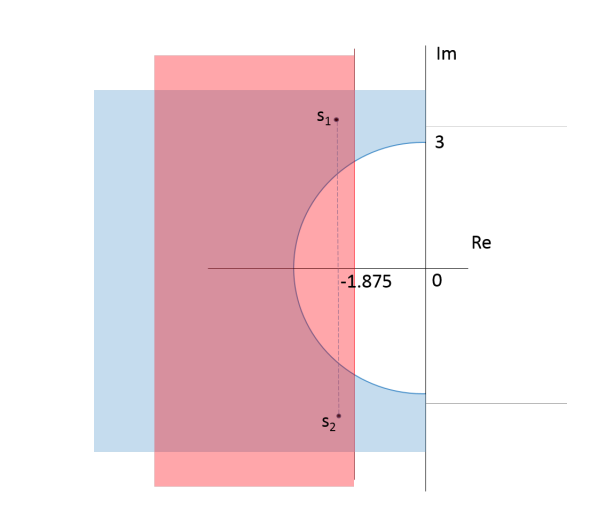
\includegraphics[width=0.65\linewidth]{figs/1.25.png}
        \caption{Locations of the Poles of \(H(s)\)}
    \label{fig:prb42}
\end{figure}
\noindent The poles of $H(s)$ are the roots of $s^2 + 4s + 16$, which can be computed to be $s_{1,2} = -2 \pm 2 \sqrt{3}$. They are plotted in the complex plane and found to be in both of shaded regions. Hence the given system satisfy these specs.

\clearpage
\subsection{Time-Domain Specs}
Consider the transfer function 
\[
H(s)=\frac{16}{s^2+4s+16}
\]
Suppose that you are given the following time-domain specs: $t_r \leq 0.6$, $t_s \leq 1.6$ (defined by the time system's response reach and stay within $5\%$ of steady state). Suppose additionally, we have overshoot: $M_p \leq \frac{1}{e^2}$. Does the given system satisfy these specs? \\
\textbf{\textcolor{red}{Solution :}} \\
Recall that $t_r=\frac{1.8}{\omega_n}$, $t_s=\frac{3}{\sigma}$ and $M_p =e^{-\frac{\zeta \pi}{\sqrt{1-\zeta^2}}}=e^{-\pi \arctan \theta}$. Therefore by the given specs $t_r \leq 0.6$, $t_s \leq 1.6$ and  $M_p \leq \frac{1}{e^2}$, we can conclude that:
\[
\omega_n \geq 3 \text{, and  } \sigma \geq 1.875 \text{, and  }  \theta \geq 42^\circ
\]
The admissible region due to overshoot constraint is plotted as the yellow shaded area in the figure given below. Since the poles of the system are not in the yellow region, the given system does not satisfy the specs.
\begin{figure}[H]
    \centering
    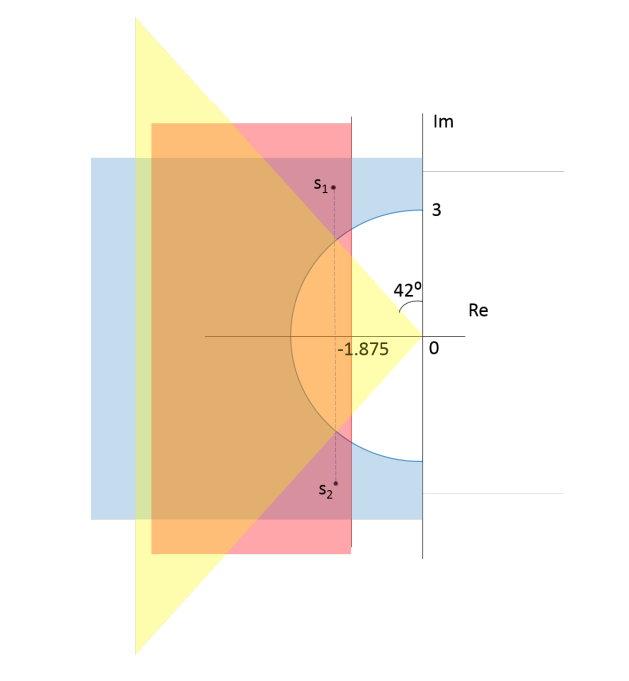
\includegraphics[width=0.65\linewidth]{figs/1.26.png}
    \caption{Admissible Region}
    \label{fig:prb43}
\end{figure}

\clearpage
\subsection{Second-Order Systems}

Consider a second-order system with peak time $t_p = 0.5$ sec. and $5\%$ settling time $t_s = 1.5$ sec. Determine the poles of this system. \\
\textbf{\textcolor{red}{Solution :}} \\
The poles of this system are given by $s= -\sigma \pm j \omega_d$ where $\sigma=\zeta \omega_n$ and $\omega_d=\omega_n \sqrt{1-\zeta^2}$.

Given information $t_p = 0.5$ sec and $5\%$ settling time $t_s = 1.5$ sec leads to $\omega_d=2 \pi$ and $\sigma=2$. Therefore the poles of the system are $s=-2 \pm 2 \pi $

\clearpage
\subsection{Time-Domain Specs}

Consider a second-order system with peak time $t_p = 0.5$ sec. and $5\%$ settling time $t_s = 1.5$ sec. Does this system satisfy rising time $t_r \leq 0.18$ sec? \\
\textbf{\textcolor{red}{Solution :}} \\
Recall that $t_r=\frac{1.8}{\omega_n}$. Therefore this system must have $\omega_n \geq 10$ in order to satisfy the rise time requirement. 

We know that $\omega_n^2 =\sigma^2 +\omega_d^2$. Given that $t_p = 0.5$ sec and $5\%$ settling time $t_s = 1.5$ sec, we can compute the corresponding $\omega_d=2 \pi$ and $\sigma=2$. 

Therefore this system's $\omega_n^2 = 2^2 + (2 \pi)^2 =68$. Since $\omega_n^2 < 100$, therefore this system can't satisfy $t_r \leq 0.18$ sec.  

\clearpage
\section{Stability}
\subsection{Stability Analysis}
In a feedback control loop, the open-loop transfer function \(G(s)\) and the controller \(C(s)\) are given by
\begin{equation}
G(s) = \frac{s - 2}{(s - 1)(s + 4)}, \quad C(s) = K \frac{s + 1}{s}
\end{equation}
Determine \(K \in \mathbb{R}\), if exists, such that the control loop is stable.


\textbf{\textcolor{red}{Solution :}} \\  
% Short Answer: No valid range
% Reasoning Steps:
The closed-loop characteristic polynomial is given by the numerator of \(1 + G(s)C(s)\), i.e.,
\begin{equation}
p(s) = s^3 + (3 + K)s^2 - (K + 4)s - 2K
\end{equation}
On applying the Routh criterion, we observe that \(p(s)\) has all its roots in the open Left Half Plane (LHP) if and only if the following three conditions are simultaneously satisfied:
\begin{equation}
3 + K > 0
\end{equation}
\begin{equation}
K^2 + 5K + 12 < 0
\end{equation}
\begin{equation}
-2K > 0
\end{equation}
The first and third conditions require that \(-3 < K < 0\). On the other hand, the second condition can be re-written as \((K + 2.5)^2 + 5.75 < 0\). This form allows us to see that the condition cannot be met by any real value of \(K\). In summary, there is no real value for \(K\) which stabilizes the closed loop.
%Problem End

\clearpage
\subsection{Stability Analysis using PI Controller}

Consider a plant with a nominal transfer function given by
\begin{equation}
G(s) = \frac{1}{(s - 1)^2}
\end{equation}
Prove that this system cannot be stabilized with a \(PI\) controller.

\textbf{\textcolor{red}{Solution :}} \\ 
% Short Answer: NA
% Reasoning Steps:
We consider the general form of a PI controller as
\begin{equation}
C(s) = \frac{as + b}{s}
\end{equation}
Thus, the closed-loop characteristic polynomial, \(A_{cl}(s)\), is given by
\begin{equation}
A_{cl}(s) = \text{numerator of } \{1 + G(s)C(s)\} = s^3 - 2s^2 + (1 + a)s + b
\end{equation}
Hence, there are no values for \(a\) and \(b\) such that \(A_{cl}(s)\) is strictly Hurwitz. This originates from the fact that one of the coefficients of the polynomial \(A_{cl}(s)\) is negative no matter what values we choose for \(a\) and \(b\).
% Problem End

\clearpage
\subsection{Designing Minimal Complexity Stabilizing Controller}
Consider a continuous time system with a transfer function \(G_o(s)\) defined as
\begin{equation}
G_o(s) = \frac{2}{(s - 1)(s + 2)} = \frac{2}{s^2 + s - 2}.
\end{equation}
Your task is to design a controller of minimal complexity that stabilizes the plant, ensures zero steady state error for step disturbances, and achieves a closed-loop response where natural modes decay at a rate no slower than \(e^{-3t}\).

\textbf{\textcolor{red}{Solution :}} \\ 
% Short Answer: \(C(s) = \frac{35.5s^2 + 114.5s + 90}{s^2 + 14s}\)
% Reasoning Steps:
We begin by recalling that we can choose an arbitrary set of closed loop natural frequencies if the closed loop characteristic polynomial, $A_{cl}(s)$, has degree at least equal to $2n-1$ (the degree of $A_o(s)$, the plant nominal model denominator). However, since we want to force zero steady state error at d.c., an additional degree-of-freedom is needed. We are aiming for a minimum complexity controller; hence, we choose the degree of $A_{cl}(s)$ equal to $4$.

In addition, the roots of $A_{cl}(s)$ should be to the left of $s = -3$ to ensure that the response time specification is met. Say we choose
\begin{equation}
A_{cl}(s) = (s^2 + 6s + 9)(s + 4)(s + 5) = s^4 + 15s^3 + 83s^2 + 201s + 180
\end{equation}
We can now solve the Diophantine equation
\begin{equation}
(s - 1)(s + 2) \underbrace{s(s + l_0)}_{L(s)} + 2 \underbrace{(p_2s^2 + p_1s + p_0)}_{P(s)} = s^4 + 15s^3 + 83s^2 + 201s + 180
\end{equation}
where $A_o(s)$ is the plant nominal model denominator, $B_o(s)$ is the plant numerator, $L(s)$ represents the controller's pole polynomial, and $P(s)$ represents the controller's zero polynomial.
We finally obtain
\begin{equation}
P(s) = 35.5s^2 + 114.5s + 90
\end{equation}
\begin{equation}
L(s) = s^2 + 14s
\end{equation}
\begin{equation}
C(s) = \frac{35.5s^2 + 114.5s + 90}{s^2 + 14s}
\end{equation}
% Problem End

\clearpage
\subsection{Pole Assignment}

Consider a nominal model given by
\begin{equation}
G_o(s) = \frac{1}{(s + 1)^2}
\end{equation}
Further assume that we need zero steady state error at zero frequency. We want to specify a third order polynomial $A_{cl}(s)$. From our analysis of the pole assignment methodology, we know that not every third order $A_{cl}(s)$ can achieve stable closed loop. Find the family of stable third degree polynomials that yields a stable closed loop with zero steady state error at d.c. Define the closed-loop system's characteristic equation as \(A_{cl}(s) = s^3 + a_2s^2 + a_1s + a_0\). Determine the conditions for the coefficients \(a_2\), \(a_1\), and \(a_0\) such that the closed-loop system is stable and achieves the required steady state error characteristics.

\textbf{\textcolor{red}{Solution :}}\\
% Short Answer: "For stability and zero steady state error, the coefficients must satisfy the following conditions: \(a_2 - 2 = 0\), \(a_0 > 0\), \(a_1 > 0\), \(2a_1 - a_0 > 0\)."
% Reasoning Steps:
Define
\begin{equation}
A_{cl}(s) = s^3 + a_2s^2 + a_1s + a_0
\end{equation}
Then, the degree of $L(s)$ must be one and, to satisfy the steady state requirement, it must have integration. Hence the controller has the form
\begin{equation}
C(s) = \frac{p_1s + p_0}{s}
\end{equation}
The pole assignment equation is
\begin{equation}
A_o(s)L(s) + B_o(s)P(s) = s^3 + a_2s^2 + a_1s + a_0
\end{equation}
\begin{equation}
s(s + 1)^2 + (p_1s + p_0) = s^3 + a_2s^2 + a_1s + a_0
\end{equation}
\begin{equation}
s^3 + 2s^2 + (p_1 + 1)s + p_0 = s^3 + a_2s^2 + a_1s + a_0
\end{equation}
From this we see that $a_2 = 2$ assures integration in the controller. Furthermore, since $A_{cl}(s)$ has to be stable, conditions to satisfy this requirement can be obtained using Routh's Algorithm applied to the polynomial $A_{cl}(s) = s^3 + 2s^2 + a_1s + a_0$. The algorithm yields $A_{cl}$ stable if and only if
\begin{equation}
2a_1 > a_0
\end{equation}
\begin{equation}
a_0 > 0
\end{equation}
Finally, the family of polynomials satisfying both, stability and integration, is
\begin{equation}
\mathcal{A} = \{s^3 + 2s^2 + a_1s + a_0 \in \mathbb{R}^3[s] : a_0 > 0, a_1 > 0, 2a_1 - a_0 > 0\}
\end{equation}
where $\mathbb{R}^3[s]$ is the ring of polynomials in $s$ of degree less or equal to three, with real coefficients.
% Problem End 

\clearpage
\subsection{Stability of Equilibrium}

Consider an ODE 
\begin{equation}
    \begin{cases}
        &\dot{x} = xy, \\
        &\dot{y} = -y + u
    \end{cases}
\end{equation}


where \(u\) is the input. Here we are interested in the stability of the equilibrium solution \((0,0)\). Consider a linear feedback of the form \(u = ax + by\). Can the linearization about the equilibrium be made asymptotically stable for any choice of constants \((a,b)\)?\\

\textbf{\textcolor{red}{Solution :}} \\
% Short Answer: No
% Reasoning Steps:
Substituting the feedback into the system yields
\begin{align*}
    \dot{x} &= xy, \\
    \dot{y} &= -y + ax + by.
\end{align*}

The linearization of the system about the equilibrium point \((0,0)\) is represented by the Jacobian matrix
\[
J = \begin{bmatrix}
    0 & 0 \\
    a & b-1
\end{bmatrix}.
\]

The stability of the equilibrium is determined by the eigenvalues of \(J\), which are solutions to the characteristic equation
\[
\det(J - \lambda I) = 0,
\]
resulting in eigenvalues \(\lambda_1 = 0\) and \(\lambda_2 = b-1\).

For asymptotic stability, all eigenvalues must have strictly negative real parts. However, \(\lambda_1 = 0\) does not satisfy this criterion, indicating that the equilibrium \((0,0)\) cannot be made asymptotically stable through any choice of constants \((a,b)\).
% Problem End

\clearpage
\subsection{Routh-Hurwitz Stability}


A system has a characteristic equation given by
\begin{equation}
    s^3 + Ks^2 + (K+1)s + 6 = 0.
\end{equation}

Determine the range of \(K\) for a stable system. You can use Routh-Hurwitz Stability Criteria.\\


\textbf{\textcolor{red}{Solution :}} \\
% Short Answer: The range of \(K\) for a stable system is \(K > 2\)
% Reasoning Steps:
The Routh array is structured as follows:
\begin{align*}
    s^3 & : 1 \quad K+1 \\
    s^2 & : K \quad 6 \\
    s^1 & : b \quad 0 \\
    s^0 & : 6 \\
\end{align*}
where \(b = \frac{K(K + 1) - 6}{K}\) for the \(s^1\) row. For stability, we require \(K > 0\) and \(b > 0\). Therefore, using the condition that \(b > 0\), we obtain
\begin{equation}
    K^2 + K - 6 > 0,
\end{equation}
and solving for \(K\) yields \(K > 2\) and \(K < -3\). We select \(K > 2\), since we also have the condition that \(K > 0\).
% Problem End

\clearpage
\subsection{Routh-Hurwitz Stability}


A system has the second-order characteristic equation
\begin{equation}
    s^2 + as + b = 0,
\end{equation}
where \(a\) and \(b\) are constant parameters. Determine the necessary and sufficient conditions for the system to be stable. Is it possible to determine the stability of a second-order system just by inspecting the coefficients of the characteristic equation?\\


\textbf{\textcolor{red}{Solution :}} \\
% Short Answer: The system is stable if \(a > 0\) and \(b > 0\).
% Reasoning Step
The characteristic equation is $s^2 + as + b = 0$, so, the Routh array is
\begin{align*}
    s^2 & : 1 \quad b \\
    s^1 & : a \quad 0 \\
    s^0 & : b
\end{align*}
The system is stable if and only if $a > 0$ and $b > 0$. For a second-order system, a necessary and sufficient condition for stability is that all the coefficients have the same sign.

% Problem End

\clearpage
\subsection{Assessing Stability}

A system has poles at \(-1\) and \(-5\) and zeros at \(1\) and \(-2\). Is this system stable?

\textbf{\textcolor{red}{Solution :}} \\
The system is stable since the poles are the roots of the system characteristic equation which have negative real parts. The fact that the system has a zero with a postive real part does not affect its stability.

\clearpage
\subsection{Routh-Hurwitz Stability}

Determine if the following characteristic equation has any roots with positive real parts:
\begin{equation}
    s^4+s^3-s-1 = 0
\end{equation}

\textbf{\textcolor{red}{Solution :}} \\
Note that the coefficient of the \(s^2\) term is zero. The Routh table for this equation is 
\[
\begin{array}{l|ccc}
\quad \quad s^4 & 1 & 0 & -1 \\
\quad \quad s^3 & 1 & -1 & 0 \\
\quad \quad s^2 & 1 & -1 & \\
\quad \quad s^1 & 0 & 0 & \\
\text{new} \ s^1 & 2 & 0 & \\
\quad \quad s^0 & 0 & & \\
\end{array}
\]

The presence of the zeros in the \(s^1\) row indicates that the characteristic equation has two roots which satisfy the auxiliary equation formed from the \(s^2\) row as follows: \(s^2-1 = 0\). The roots of the equation are \(=1\) and \(-1\).
The new \(s^1\) row was formed using the coefficients from the derivative of the auxiliary equation: \(2s-0 = 0\). Since there is one change of sign, the characteristic equation has one root with a positive real part, the one at \(+1\) determine from the auxiliary equation.

\clearpage
\subsection{Routh-Hurwitz Stability}

The characteristic equation of a given system is 
\begin{equation}
    s^4+6s^3+11s^2+6s+K = 0
\end{equation}
What restrictions must be placed upon the parameter \(K\) in order to ensure that the system is stable?

\textbf{\textcolor{red}{Solution :}} \\
The Routh table for this system is 
\[
\begin{array}{l|ccc}
s^4 & 1 & 11 & K \\
s^3 & 6 & 6 & 0 \\
s^2 & 10 & K & 0 \\
s^1 & \frac{60-6K}{10} & 0 & \\
s^0 & K & & \\
\end{array}
\]
For the system to be stable. \(60-6K>0\). or \(K<10\), and \(K>0\). Thus \(0<K<10\).

\clearpage
\subsection{Routh-Hurwitz Stability}

Construct a Routh table and determine the number of roots with positive real parts for the equation
\begin{equation}
    2s^3+4s^2+4s+12 = 0
\end{equation}

\textbf{\textcolor{red}{Solution :}} \\
The Routh table for this equation is given below. Here the \(s^2\) row was divided by \(4\) before the \(s^1\) row was computed. The \(s^1\) row was then divided by \(2\) before the \(s^0\) was computed.
\[
\begin{array}{l|cc}
s^3 & 2 & 4  \\
s^2 & 1 & 3 \\
s^1 & -1 & 0  \\
s^0 & 3 &  \\
\end{array}
\]
Since there are two changes of sign in the first column of the Routh table, the equation above has two roots with positive real parts.

\clearpage
\subsection{Routh-Hurwitz Stability}

Use Hurwitz stability and show that for what range of values of \(K\) is the system with the following characteristic equation stable?
\begin{equation}
    s^2 + Ks +2K-1 = 0
\end{equation}

\textbf{\textcolor{red}{Solution :}} \\
The Hurwitz determinants for this system are
\begin{equation}
    \Delta_2 = 
\begin{vmatrix}
K & 0 \\
1 & 2K-1 \\
\end{vmatrix} = 2K^2-K = K(2K-1) \quad \Delta_1 = K
\end{equation}
In order for these determinants to be positive, it is necessary that \(K>0\) and \(2K-1>0\). Thus the system is stable if \(K>\frac{1}{2}\).

\clearpage
\subsection{Routh-Hurwitz Stability}

Determine the Hurwitz conditions for stability of the following general fourth-order characteristic equation, assuming \(a_4\) is positive.
\begin{equation}
    a_4s^4 + a_3s^3 + a_2 s^2 + a_1 s + a_0 = 0
\end{equation}

\textbf{\textcolor{red}{Solution :}} \\

The Hurwitz determinants are:
\begin{align*}
\Delta_1 &= a_3, \\
\Delta_2 &= a_3a_2 - a_4a_1, \\
\Delta_3 &= \begin{vmatrix} a_3 & a_1 & 0 \\ a_4 & a_2 & a_0 \\ 0 & a_3 & a_1 \end{vmatrix}, \\
\Delta_4 &= \begin{vmatrix} a_3 & a_1 & 0 & 0 \\ a_4 & a_2 & a_0 & 0 \\ 0 & a_3 & a_1 & 0 \\ 0 & a_4 & a_2 & a_0 \end{vmatrix}.
\end{align*}

For the system to be stable:
\[
\Delta_1 > 0, \quad \Delta_2 > 0, \quad \Delta_3 > 0, \quad \Delta_4 > 0
\]

\clearpage
\subsection{Characterisitic Equation}


Prove that a continuous system is unstable if any coefficients of the characteristic equation are zero.

\textbf{\textcolor{red}{Solution :}} \\
The characteristic equation may be written in the form
\begin{equation}
    (s-s_1)(s-s_2)(s-s_3)\cdots (s-s_n) = 0
\end{equation}\
where \(s-1,s_2,\cdots,s_n\) are the roots of the equation. If this equation is multiplied out, \(n\) new equations an be obtained relating the roots and the coefficients of the characteristic equation in the usual form. Thus
\begin{equation}
    a_n s^n + a_{n-1}s^{n-1} + \cdots + a_0 = 0
\end{equation}
and the relations are 
\begin{equation}
    \frac{a_{n-1}}{a_n} = - \sum_{i=1}^n s_i, \frac{a_{n-2}}{a_n} =  \sum_{i=1}^n \sum_{\substack{j=1 \\ i \neq j}}^n s_i s_j,\frac{a_{n-3}}{a_n} - \sum_{i=1}^n \sum_{j=1}^n \sum_{\substack{k=1 \\ i \neq j \neq k}}^n s_i s_j s_k, \cdots,\frac{a_0}{a_n}(-1)^n s_1 s_2 \cdots s_n
\end{equation}
The coefficients \(a_{n-1},a_{n-2},\cdots,a_0\) all have the same sign as \(a_n\) and are nonzero if all the roots \(s_1,s_2,\cdots,s_n\) have negative real parts. The only way any one of the coefficients can be zero is for one or more of the roots to have zero or positive real parts. In either case, the system would be unstable.

\clearpage
\subsection{Assessing Stability (Discrete-time system)}

What is the transfer function of a discrete system with a gain factor of 2, zeros at 0.2 and -0.5, and poles at 0.5, 0.6, and -0.4? Is it stable?

\textbf{\textcolor{red}{Solution :}} \\
The transfer function is
\[ P(z) = \frac{2(z - 0.2)(z + 0.5)}{(z - 0.5)(z - 0.6)(z + 0.4)} \]
Since all the system poles are inside the unit circle, the system is stable.

\clearpage
\subsection{Identifying Singular Points in ODEs}

Find the singular points of the pair of equations
\[
\frac{dx_1}{dt} = \sin x_2 \quad \text{and} \quad \frac{dx_2}{dt} = -x_1 + x_2
\]
\textbf{\textcolor{red}{Solution :}} \\
Singular points are found by setting \(\frac{dx_1}{dt} = 0\) and \(\frac{dx_2}{dt} = 0\). The first equation is satisfied by
\[ x_2 =  n\pi, \quad n = 0, 1, 2, \ldots \]
The second is satisfied by \(x_1 = x_2\). Hence the singular points are defined by
\[ x_1 =  n\pi, \quad x_2 =  n\pi, \]
where \(n = 0, 1, 2, \ldots\)

\clearpage
\subsection{Stability and Time Constant}

For each of the systems below:
\begin{itemize}
    \item What are the poles? Is the system stable?
    \item What is the time constant associated with each pole? Which time constant is the slowest? (Provide a time constant regardless of stability.)
\end{itemize}
\begin{itemize}
    \item[(a)] \(G(s) = \frac{s-2}{s+7}\)
    \item[(b)] \(G(s) = \frac{s+2}{s-7}\)
    \item[(c)] \(G(s) = \frac{-9}{s^2+2s-8}\)
    \item[(d)] \(G(s) = \frac{5}{(s^2+4s+13)(s-5)}\)
\end{itemize}
\textbf{\textcolor{red}{Solution :}} \\
\begin{itemize}
    \item[(a)] 
    \textbf{Poles:} \(s = -7 \quad \text{system is stable}\)\\
    \textbf{Time constant:} \(\tau = \frac{1}{|Re(s)|} = \frac{1}{7}\) sec
    \item[(b)] 
    \textbf{Poles:} \(s = 7 \quad \text{system is unstable}\)\\
    \textbf{Time constant:} \(\tau = \frac{1}{|Re(s)|} = \frac{1}{7}\) sec
    \item[(c)] 
    \textbf{Poles:} \(s_1 = -4, s_2 = 2 \quad \text{system is unstable}\)\\
    \textbf{Time constant:} \(\tau_1 = \frac{1}{|Re(s)|} = \frac{1}{4}\) sec, \(\tau_2 = \frac{1}{|Re(s)|} = \frac{1}{2}\) sec, \(\tau_2\) is slowest time constant
    \item[(d)]
    \textbf{Poles:} \(s_{1,2} = -2 \pm 3j, s_3 = +5 \quad \text{system is unstable}\)\\
    \textbf{Time constant:} \(\tau_{1,2} = \frac{1}{|Re(s)|} = \frac{1}{2}\) sec, \(\tau_3 = \frac{1}{|Re(s)|} = \frac{1}{5}\) sec, \(\tau_{1,2}\) is slowest time constant
\end{itemize}
\clearpage

\clearpage
\subsection{Observer}

Consider the single-input, single-output transfer function:
$$
Y(s)=\frac{s+1}{s^2+2 s+2} U(s)
$$
\begin{itemize}
    \item [(a)] Find a second-order state-space model that represents this transfer function.
    \item [(b)] For this state-space model, calculate a state-feedback controller $u=-K x+r$ that places the closed-loop poles at -4 and -25.
    \item [(c)] Construct an observer to estimate $x$ based on the known inputs $u$ and observations $y$ (put the observer poles at $\{-50,-51\}$).
    \item [(d)] With the controller and observer from the previous problems in place, calculate $k_r$ such that $u=-K \hat{x}+k_r r$ yields a closed-loop system $Y / R$ with unity gain.
\end{itemize}

\textbf{\textcolor{red}{Solution :}} \\
\begin{itemize}
    \item [(a)] Recall that for a transfer function:
$$
\frac{Q(s)}{P(s)}=\frac{b_0 s^n+b_1 s^{n-1}+\cdots+b_{n-1} s+b_n}{s^n+a_1 s^{n-1}+\cdots+a_{n-1} s+a_n}
$$
the controllable canonical realization is:
$$
\begin{aligned}
A & =\left[\begin{array}{ccccc}
0 & 1 & 0 & \ldots & 0 \\
0 & 0 & 1 & \ldots & 0 \\
\vdots & \vdots & \vdots & & \vdots \\
0 & 0 & 0 & \ldots & 1 \\
-a_n & -a_{n-1} & -a_{n-2} & \ldots & -a_1
\end{array}\right] \\
B & =\left[\begin{array}{llllll}
0 & 0 & \ldots & 1
\end{array}\right]^T \\
C & =\left[\begin{array}{lllll}
b_n-a_n b_0 & b_{n-1}-a_{n-1} b_0 & b_{n-2}-a_{n-2} b_0 & \ldots & b_1-a_1 b_0
\end{array}\right] \\
D & =\left[b_0\right]
\end{aligned}
$$

Here $b_0=0$ and therefore we have that
$$
\begin{aligned}
& \dot{x}=\left[\begin{array}{cc}
0 & 1 \\
-2 & -2
\end{array}\right] x+\left[\begin{array}{l}
0 \\
1
\end{array}\right] \\
& y=\left[\begin{array}{ll}
1 & 1
\end{array}\right]
\end{aligned}
$$
\item [(b)] If we want to place the closed loop poles at -4 and -25 , then the new denominator would be $(s+4)(s+25)=s^2+29 s+100$. Therefore, $a_0+k_1=100 \Longrightarrow k_1=100-2=98$ and $a_1+k_2=29 \Longrightarrow k_2=29-2=27$. Hence, $K=\left[\begin{array}{ll}98 & 27\end{array}\right] \Longrightarrow u=-\left[\begin{array}{ll}98 & 27\end{array}\right] x+r$.
\item [(c)] For an observer gain $L$, the observer poles are the eigenvalues of $A \quad L C$, which coincide with the eigenvalues of $A^T-C^T L^T$. Consequently to compute the observer gain in MAT$\mathrm{LAB}$, we apply the place command for $\left(A^T, C^T\right)$. It is a rule of thumb, to pick observer poles to be 2-5 times further than the controller poles. Suppose we want to place the observer poles at $\{-50,-51\}$. By using the MATLAB command
$$ L=\operatorname{place}\left(A^{\prime}, C^{\prime},[-50,-51]\right) $$
where $\left(A^T, C^T\right)$ are as above we get $L=\left[\begin{array}{ll}-2449 & 2548\end{array}\right]^T$.

\item [(d)] To obtain $k_r$, recall that $\hat{x}(t) \equiv 0$ if $\hat{x}(0) = 0$, so we can ignore the observer. The closed loop system transfer function disregards initial conditions. With full state feedback, the
closed loop transfer function is
$$\frac{Y(s)}{R(s)}=C [s I-(A- B K)]^{-1}B k_r$$
To set the DC gain to unity we need
$$1 = C [s I-(A- B K)]^{-1}B k_r \implies  k_r = 100$$

\end{itemize}
\clearpage

\subsection{Discrete-Time Implementation}
Consider the following plant:
$$
\dot{y}+5 y=3 u
$$
Suppose a PI controller is used with P gain $K_p$ and I gain $K_i$. Assume the closed-loop system is stable. Then what sampling time would you recommend for a discrete-time implementation? Write out $\Delta t$ as a function of $K_p$ and $K_i$. Use $u(t)=k_p e(t)+K_i \int_0^t e(\tau) d \tau$ with $e(t)=r(t)-y(t)$. \\

\textbf{\textcolor{red}{Solution :}} \\
Since we are using PI control, $u(t)=k_p e(t)+K_i \int_0^t e(\tau) d \tau$ with $e(t)=r(t)-y(t)$. The closed loop system can be expressed as:
$$ \ddot{y}+\left(5+3 K_p\right) \dot{y}+3 K_i y=3 K_p \dot{r}+3 K_i r . $$

\noindent Performing Laplace transform on both sides, we have the closed-loop transfer function
$$
T(s)=\frac{3 K_p s+3 K_i}{s^2+\left(5+3 K_p\right) s+3 K_i} .
$$

\noindent The poles of the closed-loop system is
$$
s_{1,2}=\frac{-\left(5+3 K_p\right) \pm \sqrt{\left(5+3 K_p\right)^2-12 K_i}}{2} .
$$

\noindent Now we need to consider the following two scenarios:
(i) If $\left(5+3 K_p\right)^2-12 K_i \geq 0, s_1$ and $s_2$ are both real, the corresponding time constant is $\tau_1=\frac{2}{\left|-\left(5+3 K_p\right)+\sqrt{\left(5+3 K_p\right)^2-12 K_i}\right|}, \tau_2=\frac{2}{\left(5+3 K_p\right)+\sqrt{\left(5+3 K_p\right)^2-12 K_i}}$. For $\tau_1$, we have
$$
\Delta t_1=\frac{1}{5 \mid\left(5+3 K_p\right)-\sqrt{\left(5+3 K_p\right)^2-12 K_i}},
$$

For $\tau_2$, we have
$$
\Delta t_2=\frac{1}{5\left(5+3 K_p\right)+5 \sqrt{\left(5+3 K_p\right)^2-12 K_i}} .
$$

\noindent Since $\Delta t_2 \leq \Delta t_1$, we can choose $\Delta t=\Delta t_2$.
(ii) If $\left(5+3 K_p\right)^2-12 K_i \geq 0, s_1$ and $s_2$ are a complex conjugate, which has same real part and hence same time constant $\tau=\frac{2}{5+3 K_p}$. In this case, we should design $\Delta t=\frac{1}{10} \frac{2}{5+3 K_p}=$ $\frac{1}{25+15 K_p}$.
\clearpage

\section{Time Response of Dynamical Systems}
\subsection{Steady-State Response}

Consider a second-order linear system described by the following ordinary differential equation (ODE):

            \begin{equation*}
                a\ddot{x}(t) + b\dot{x}(t) + cx(t) = \cos(3t) + 2\sin(4t), \quad x(0) = 0, \quad \dot{x}(0) = 0,
            \end{equation*}
            
            where \( a \), \( b \), and \( c \) are positive real numbers. The system is known to have a steady-state response of the form:

            \begin{equation*}
                x_{ss}(t) = A\cos(3t - \phi_1) + B\sin(4t - \phi_2),
            \end{equation*}
            
            where \( A \), \( B \), \( \phi_1 \), and \( \phi_2 \) are constants.
            
            Determine the values of \( a \), \( b \), and \( c \) given that \( A = \frac{1}{3\sqrt{2}} \), \( B = \frac{1}{2\sqrt{2}} \), \( \phi_1 = \frac{\pi}{4} \), and \( \phi_2 = \frac{3\pi}{4} \).


\textbf{\textcolor{red}{Solution :}} \\
Transfer function of the system is

\begin{equation}
    G(s) = \frac{1}{as^2 + bs + c}
\end{equation}
and

\begin{align*}
    M(\omega) &= \frac{1}{\sqrt{(c-a\omega^2)^2 + (b\omega)^2}}, \\
    \phi(\omega) &= -\tan^{-1}\left(\frac{b\omega}{c-a\omega^2}\right)
\end{align*}

The steady-state response \( x_{ss}(t) \) is given by:
\begin{align*}
x_{ss}(t) &= 1 \times M(3) \times \cos(3t + \phi(3)) + 2 \times M(4) \times \sin(4t + \phi(4)) \\
&= 1 \times \frac{1}{\sqrt{(c-9a)^2 + (3b)^2}} \times \cos\left(3t - \tan^{-1}\left(\frac{3b}{c-9a}\right)\right) \\
&\quad + 2 \times \frac{1}{\sqrt{(c-16a)^2 + (4b)^2}} \times \sin\left(4t - \tan^{-1}\left(\frac{4b}{c-16a}\right)\right)
\end{align*}
Given the following conditions:
\begin{align*}
    (c-9a)^2 + (3b)^2 &= 18 \\
    (c-16a)^2 + (4b)^2 &= 32 \\
    \tan^{-1}\left(\frac{3b}{c-9a}\right) &= \frac{\pi}{4} \Rightarrow c-9a = 3b \\
   \tan^{-1}\left(\frac{4b}{c-16a}\right) &= \frac{3\pi}{4} \Rightarrow c-16a = -4b
\end{align*}

Solving these equations, we find that \( b = 1 \), \( c = 12 \), and \( a = 1 \).

\clearpage
\subsection{Free Response}

Show that any free response \(y_a(t) = \sum_{k=1}^n c_k y_k(t)\) satisfies \(\sum_{i=0}^n a_i(\frac{d'y}{dt'}) = 0\)


\textbf{\textcolor{red}{Solution :}} \\

By the definition of a fundamental set, \(y_k(t), k=1,2,\cdots,n\), satisfies \(\sum_{i=0}^n a_i(\frac{d'y_k}{dt'}) = 0\). Substituting \(\sum_{k=1}^n c_k y_k(t)\) into this differential equation yields
\begin{equation}
    \sum_{i=0}^n a_i \frac{d'}{dt'} \left[ \sum_{k=1}^n c_k y_k(t) \right] = \sum_{i=0}^n \sum_{k=1}^n a_i \frac{d'}{dt'}(c_k y_k(t)) = \sum_{k=1}^n c_k \left[ \sum_{i=0}^n a_i \frac{d'y_k(t)}{dt'}\right] = 0
\end{equation}
The last equality is obtained because the term in the brackets is zero for all \(k\).

\clearpage
\subsection{Free Response}

Find the free response of the differential equation
\begin{equation}
    \frac{d^3y}{dt^3} + 4 \frac{d^2y}{dt^2} + 6 \frac{dy}{dt} + 4y = u
\end{equation}

with initial conditions \(y(0)=1, (dy/dt)|_{t=0} = 0\) and \((d^2y/dt^2)|_{t=0} = -1\)

\textbf{\textcolor{red}{Solution :}} \\
Fundamental set for this equation is \(e^{-3t},e^{-t}\cos t,e^{-t}\sin t\). Hence the free response can be written as 
\begin{equation}
    y_a(t) = c_1 e^{-2t} + c_2 e^{-t}\cos t + c_3 e^{-t} \sin t
\end{equation}
The intial conditions provide the following set of algebraic equatinos for \(c_1,c_2,c_3\):
\begin{equation}
    y_a(0) = c_1 + c_2 = 1 \quad \frac{dy_a}{dt}|_{t=0} = -2c_1 -c_2 + c_3 = 0 \quad \frac{d^2y_a}{dt^2}|_{t=0} = 4c_1 -2 c_3 = -1
\end{equation}
fro which \(c_1 = \frac{1}{2}, c_2 = \frac{1}{2}, c_3 = \frac{3}{2}\). Therefor the free response is 
\begin{equation}
    y_a(t) = \frac{1}{2}e^{-2t} + \frac{1}{2} e^{-t}\cos t + \frac{3}{2} e^{-t} \sin t
\end{equation}

\clearpage
\subsection{Inputs for Unbounded Outputs in Systems}

Determine a bounded input which will produce an unbounded output from an integrator.

\textbf{\textcolor{red}{Solution :}} \\
For example, the input \(u = 1\) will produce the output \(y=t\), which is unbounded. 

\clearpage
\subsection{Step Response}

What is the unit step response of a continuous system whose transfer function has a zero at \(-1\), a pole at \(-2\), and a gain factor of \(2\)?

\textbf{\textcolor{red}{Solution :}} \\
The Laplace transform of the output is given by \(Y(s) = P(s) U(s)\). Here 
\begin{equation}
    P(s) = \frac{2(s+1)}{s+2} \quad U(s)  =\frac{1}{s} \quad Y(s) = \frac{2(s+1)}{s(s+2)} = \frac{1}{s} + \frac{1}{s+2}
\end{equation}
Evaluating the inverse transform of the partial fraction expansion of \(Y(s)\) gives \(y(t) = 1 + e^{-2t}\)

\clearpage
\subsection{Steady State Response}

Prove that the steady state output of a stable system with transfer function \(P(s)\) and input \(u = A \sin(\omega t)\) is given by
\[ y_{ss} = A|P(j\omega)| \sin(\omega t + \phi) \quad \text{where} \quad  \phi = \arg P(j\omega) \]

\textbf{\textcolor{red}{Solution :}} \\
The Laplace transform of the output is \(Y(s) = P(s)U(s) = P(s) \left[ \frac{A\omega}{s^2 + \omega^2} \right]\).
When this transform is expanded into partial fractions, there will be terms due to the poles of \(P(s)\) and two terms due to the poles of the input \((s = \pm j\omega)\). Since the system is stable, all time functions resulting from the poles of \(P(s)\) decay to zero as time approaches infinity. Thus, the steady state output contains only the time functions resulting from the terms in the partial fraction expansion due to the poles of the input. The Laplace transform of the steady state output is therefore
\[ Y_{ss}(s) = \frac{AP(j\omega)}{2j(s-j\omega)} + \frac{AP(-j\omega)}{-2j(s+j\omega)} \]
The inverse transform of this equation is
\[ y_{ss} = A|P(j\omega)| \left[\frac{e^{j\phi} e^{j\omega t} - e^{-j\phi} e^{-j\omega t}}{2j} \right] =  A|P(j\omega)| \sin(\omega t + \phi) \quad \text{where} \quad  \phi = \arg P(j\omega) \]

\clearpage
\subsection{Unit Step Response}

The output in response to a unit step function input for a particular continuous control system is 
\[ c(t) = 1 - e^{-t}. \]
What is the delay time \(T_d\)?

\textbf{\textcolor{red}{Solution :}} \\
The output is given as a function of time. The final value of the output is \(\lim_{t \to \infty} c(t) = 1\). Hence \(T_d\) (at \(50\%\) of the final value) is the solution of 
\[ 0.5 = 1 - e^{-T_d}, \] 
and is equal to \(\log_e(2)\), or \(0.693\).

\clearpage
\subsection{Trajectory}

Show that the phase plane trajectory of the solution of the differential equation
\[ \frac{d^2x}{dt^2} + x = 0 \]
with initial conditions \(x(0) = 0\) and \(\left.\frac{dx}{dt}\right|_{t=0} = 1\) is a circle of unit radius centered at the origin.

\textbf{\textcolor{red}{Solution :}} \\
Letting \(x = x_1\) and \(x_2 = \frac{dx_1}{dt}\), we obtain the pair of equations:
\begin{align*}
\frac{dx_1}{dt} &= x_2, \quad x_1(0) = 0 \\
\frac{dx_2}{dt} &= -x_1, \quad x_2(0) = 1
\end{align*}

We eliminate time as the independent variable by writing
\[ \frac{dx_1}{dx_2} = \frac{-x_2}{x_1} \]
or
\[ x_1 dx_1 + x_2 dx_2 = 0 \]
Integrating this equation for the given initial conditions, we obtain
\[ x_1^2 + x_2^2 = 1 \]
which is the equation of a circle of unit radius centered at the origin.

\clearpage
\subsection{Time Response of ODEs}

For the given system \(G(s) = \frac{5}{s+7}\):
\begin{itemize}
    \item  What are the poles, zeros, and DC gain?
    \item  What is the general form of the free response?
    % \item  What is the general form of the forced response? 
\end{itemize}
If any poles are complex then express the free/forced response in its “real” form.

\textbf{\textcolor{red}{Solution :}} \\
\textbf{Poles:} \(s = -7\) \\
\textbf{Zeros:} No zeros \\
\textbf{DC Gain:} \(G(0) = \frac{5}{7}\) \\
\textbf{Free response:} \(y(t) = C e^{-7t}\) \\
\textbf{Forced response:} \(y_p(t)\) depends on \(u(t)\) \\

\clearpage
\subsection{Time Response of ODEs}

For the given system \(G(s) = \frac{4s-6}{s^2+2s-3}\):
\begin{itemize}
    \item  What are the poles, zeros, and DC gain?
    \item  What is the general form of the free response?
    \item  What is the general form of the forced response? 
\end{itemize}
If any poles are complex then express the free/forced response in its “real” form.

\textbf{\textcolor{red}{Solution :}} \\
\textbf{Poles:} \(s_1 = -3, s_2 = 1\) \\
\textbf{Zeros:} \(s = \frac{6}{4}\) \\
\textbf{DC Gain:} \(G(0) = \frac{-6}{-3}\) \\
\textbf{Free response:} \(y(t) = C_1 e^{-3t} + C_2 e^{t}\) \\
\textbf{Forced response:} \(y_p(t)\) depends on \(u(t)\) \\

\clearpage
\subsection{Time Response of ODEs}

For the given system \(G(s) = \frac{5}{s^2-2s+5}\):
\begin{itemize}
    \item  What are the poles, zeros, and DC gain?
    \item  What is the general form of the free response?
    \item  What is the general form of the forced response? 
\end{itemize}
If any poles are complex then express the free/forced response in its “real” form.

\textbf{\textcolor{red}{Solution :}} \\
\textbf{Poles:} \(s_{1,2} = 1 \pm 2j\) \\
\textbf{Zeros:} No zeros \\
\textbf{DC Gain:} \(G(0) = \frac{5}{5}\) \\
\textbf{Free response:} \(y(t) = C_1 e^{t} \cos(2t) + C_2 e^{t} \sin(2t)\) \\
\textbf{Forced response:} \(y_p(t)\) depends on \(u(t)\) \\

\clearpage
\subsection{Sketching Time Response}

\begin{itemize}
    \item[(a)] Roughly sketch the response for the following:
    \begin{equation}
        \dot{y}(t) + 2 y(t) = 4 u(t) \quad y(0) = 0, \quad u(t) = 3 \ \text{for all} \ t \geq 0
    \end{equation}
    \item[(b)] Roughly sketch the response for the following:
        \begin{equation}
        \dot{y}(t) - 3 y(t) = 2 u(t) \quad y(0) = 0, \quad u(t) = 1 \ \text{for all} \ t \geq 0
    \end{equation}

\end{itemize}
\textbf{\textcolor{red}{Solution :}} \\
(a)
    \begin{figure}[H]
    \centering
    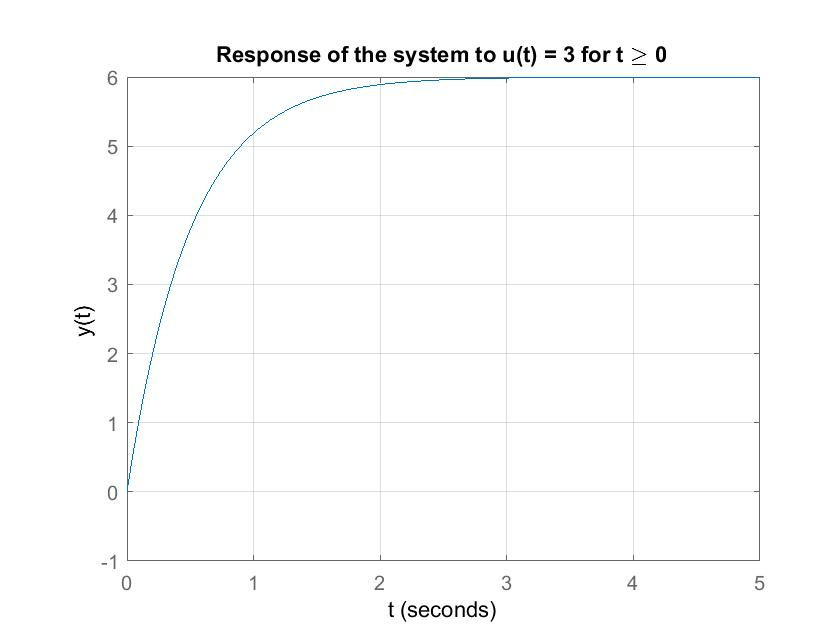
\includegraphics[width=0.5\textwidth]{figs/3.12-1.jpg}
    \caption{The system response over time.}
    \label{fig:yb}
\end{figure}
(b)
\begin{figure}[H]
    \centering
    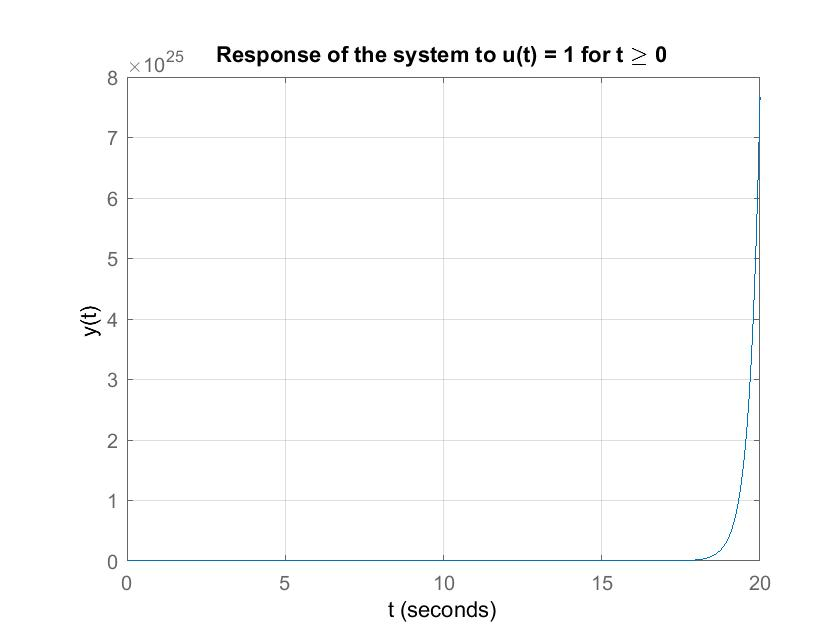
\includegraphics[width=0.5\textwidth]{figs/3.12-2.jpg}
    \caption{The system response over time.}
    \label{fig:yb}
\end{figure}

\clearpage
\subsection{Unit Step Response}

Four systems and four unit step responses are given below. Match each system to its unit step response.
\begin{itemize}
    \item[(a)] \(G_A(s) = \frac{-2s+10}{s^2+2s+5}\)
    \item[(b)] \(G_B(s) = \frac{-10s+10}{s^2+2s+5}\)
    \item[(c)] \(G_c(s) = \frac{2s+10}{s^2+2s+5} \)
    \item[(d)] \(G_D(s) = \frac{10s+10}{s^2+2s+5}\)
\end{itemize}
\begin{figure}[h]
\centering
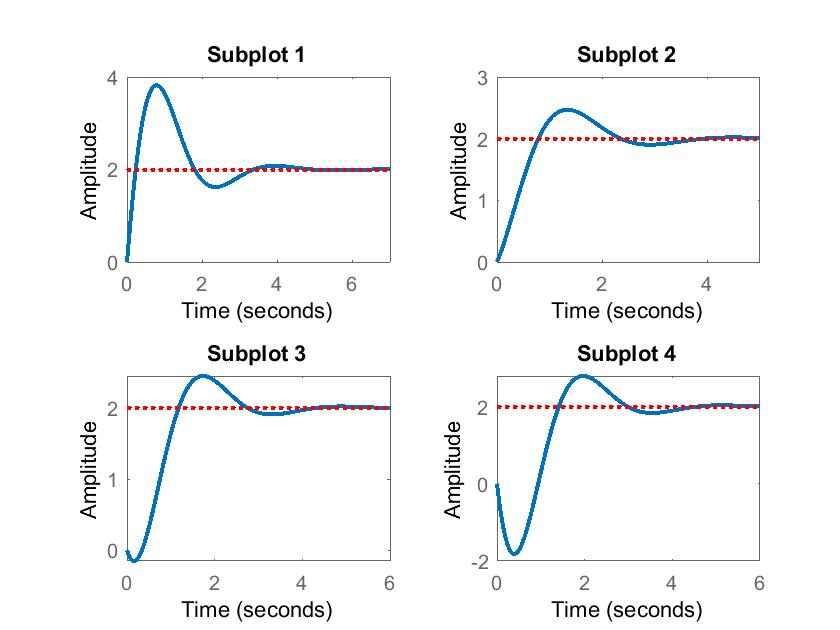
\includegraphics[width=\textwidth]{figs/3.13.jpg}
\caption{Step responses}
\end{figure}
\textbf{\textcolor{red}{Solution :}} \\
\textbf{Subplot1}: \(G_D(s)\) \\
\textbf{Subplot2}: \(G_C(s)\) \\
\textbf{Subplot3}: \(G_A(s)\) \\
\textbf{Subplot4}: \(G_B(s)\) \\

\clearpage
\subsection{Steady State Response}

For the following first-order systems with the sinusoidal input \(u(t) = 5 \sin(4t+0.1)\)
\begin{itemize}
    \item What is the magnitude and phase of \(G(j\omega)\)?
    \item Is the steady-state response bounded? If yes, what is it?
    \item[(a)] \(-2\dot{y}(t) - y(t) = 3 u(t)\)
        \item[(a)] \(-2\dot{y}(t) + y(t) = 3 u(t)\)
\end{itemize}
\textbf{\textcolor{red}{Solution :}}
\begin{itemize}
    \item[(a)] 
    \item \(G(s) = \frac{3}{-2s-1} \rightarrow s_1 = \frac{-1}{2} \rightarrow \text{system is stable}\) \\ \(\omega = 4 \rightarrow |G(4j)| = 0.37 \quad \text{and} \quad \angle G(j\omega) = 1.7 \)
    \item Yes, \(y(t) = 1.85 \sin(4t+1.8)\)
    \item[(b)]
    \item \(G(s) = \frac{3}{-2s+1} \rightarrow s_1 = \frac{1}{2} \rightarrow \text{system is unstable}\) \\ \(\omega = 4 \rightarrow |G(4j)| = 0.37 \quad \text{and} \quad \angle G(j\omega) = 1.44 \)
    \item No, response is not bounded.
\end{itemize}

\clearpage
\subsection{Steady State Response}

The figure shows the output \(y(t)\) generated by a linear system \(G(s)\) with input \(u(t) = A_0 \cos(\omega_0 t)\).
\begin{itemize}
    \item[(a)] What are the values of \(A_0\) and \(\omega_0\) for the input signal \(u(t)\)?
    \item[(b)] What is the magnitude \(|G(j\omega_0)|\)?
    \item[(c)] What is the phase \(\angle G(j\omega_0)\) in degrees?
\end{itemize}
\begin{figure}[h]
\centering
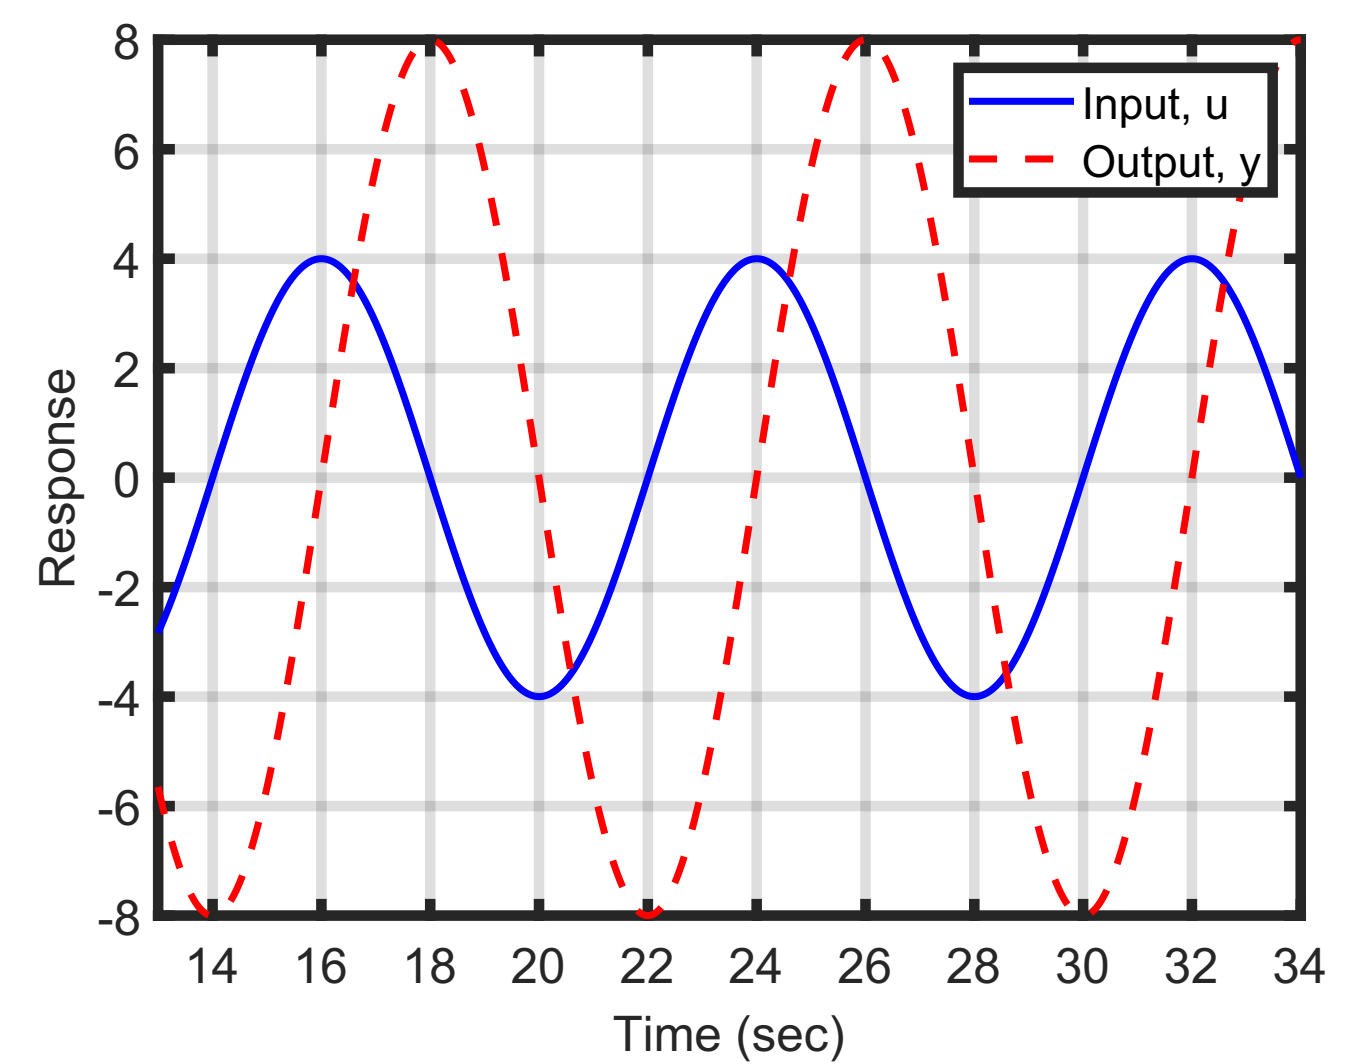
\includegraphics[width=0.7\linewidth]{figs/3.15.png}
\caption{System response}
\end{figure}
\textbf{\textcolor{red}{Solution :}}
\begin{itemize}
    \item[(a)] \(A_0 = 4\) and \(\omega_0 = \frac{\pi}{4} \quad \text{rad/sec}\)
    \item[(b)] \(|G(j\omega_0)| = 2\) 
    \item[(c)] \(\angle G(j\omega_0) = -\frac{\pi}{2}\)
\end{itemize}

\clearpage
\subsection{Zeros or Poles}

Let \(y(t)\) be the response of a stable, LTI system \(G(s)\) due to a sinusoidal input \(u(t) = \sin(2t)\). If \(y(t)\) converges back to zero in steady-state, then what can we say about the zeros or poles of \(G(s)\)?
\textbf{\textcolor{red}{Solution :}}
\[y(t) = |G(2j)|sin(2t+\angle G(2j)) = 0 \rightarrow |G(2j)| = 0\]
Which we can conclude that \(G(s)\) has a zero at \(2j\).

\clearpage
\subsection{Steady State Response}

Consider a first-order LTI system \(G(s) = \frac{b_0}{s+a_0} \) where \(a_0\) and \(b_0\) are non-zero numbers. If the phase of \(G(j\omega)\) at \(\omega = 0\) is expressed in degrees, what values can it have?

\textbf{\textcolor{red}{Solution :}}

It can only be \(0\) degrees or \(180\) degrees.

\clearpage
\subsection{Steady-State Response}

Answer the following questions.
\begin{itemize}
    \item [(a)] Consider the following system $G(s)$ and sinusoidal input:
        \begin{align*}
        & -3 \dot{y}(t)-2 y(t)=7 u(t) \\
        & u(t)=6 \cos (t+4)
        \end{align*}
    What is the magnitude and phase of $G(1 j)$ ? Is the steady-state output bounded? If yes, what is it?
    \item[(b)] Consider the following system $G(s)$ and sinusoidal input:
        \begin{align*}
        & \ddot{y}(t)+0.1 \dot{y}(t)+4 y(t)=\dot{u}(t)+2 u(t) \\
        & u(t)=-\cos (2 t)
        \end{align*}
    What is the magnitude and phase of $G(2 j)$ ? Is the steady-state output bounded? If yes, what is it?
\end{itemize}

\textbf{\textcolor{red}{Solution :}} \\
For a sinusoidal input $u(t)=A \cos (\omega t)$ an LTI system $G$ with zero initial conditions, the system output can be expressed as follows:
$$
y(t)=A|G(j \omega)| \cos (\omega t+\angle G(j \omega))
$$
\begin{itemize}
    \item [(a)]  We derive the transfer function as $G(s)=\frac{-7}{3 s+2}$. This gives $|G(j)|=\frac{7 \sqrt{13}}{13}$ and $\angle G(j)=\arctan \left(\frac{3}{-2}\right)=\pi-\arctan (3 / 2)=123.69^{\circ}$. The steady state output is bounded and can be readily obtained:
$$
y_{s s}(t)=6|G(j)| \cos (t+4+\angle G(j)) \approx 11.65 \cos (t+6.16)
$$
    \item [(b)] Here the transfer function is given by
        $$ G(s)=\frac{s+2}{s^2+0.1s+4} $$
and so $|G(2j)| = 10 \sqrt{2}$ and $\angle G(2j) = \frac{-\pi}{4}$. Again, the steady state output is bounded and given by:
$$y_{ss}(t)=-10\sqrt{2}\cos{\left( 2 t -\frac{\pi}{4} \right)}$$
\end{itemize}

\clearpage
\subsection{Unbounded Response}
Consider the transfer function
\[
G(s)=\frac{1}{s^2+\omega_n^2} \qquad \omega_n >0
\]
and the input $u(t) = sin(\omega t)$,  $\omega>0$. What value of $\omega$ in $u(t)$ leads to an unbounded response and why it does so? \\

\textbf{\textcolor{red}{Solution :}} \\
\[
G(s)=\frac{1}{s^2+\omega_n^2} \implies G(j \omega) =\frac{1}{(j \omega)^2 +\omega_n^2}  =\frac{1}{\omega_n^2 - \omega^2}
\]
$\implies |G(j \omega)| =\left| \frac{1}{\omega_n^2 - \omega^2}\right| \rightarrow \infty$ when $\omega \rightarrow \omega_n$.

\clearpage
\subsection{Step Response}
Consider the following transfer function:
\[
G(s)=\frac{20 e^{-s}}{0.5s+1}
\]
Plot the step response of this system. Identify anything unusual or different in the response and report the reason for this behaviour. \\ 
\noindent 
\textbf{\textcolor{red}{Solution :}} \\
The step response of the given system can be interpreted as the step response of the transfer function \(G(s) = \frac{20}{0.5s+1}\), followed by the application of the effect of \(e^{-s}\), which shifts the response by 1 second.

\begin{figure}[h!]
    \centering
    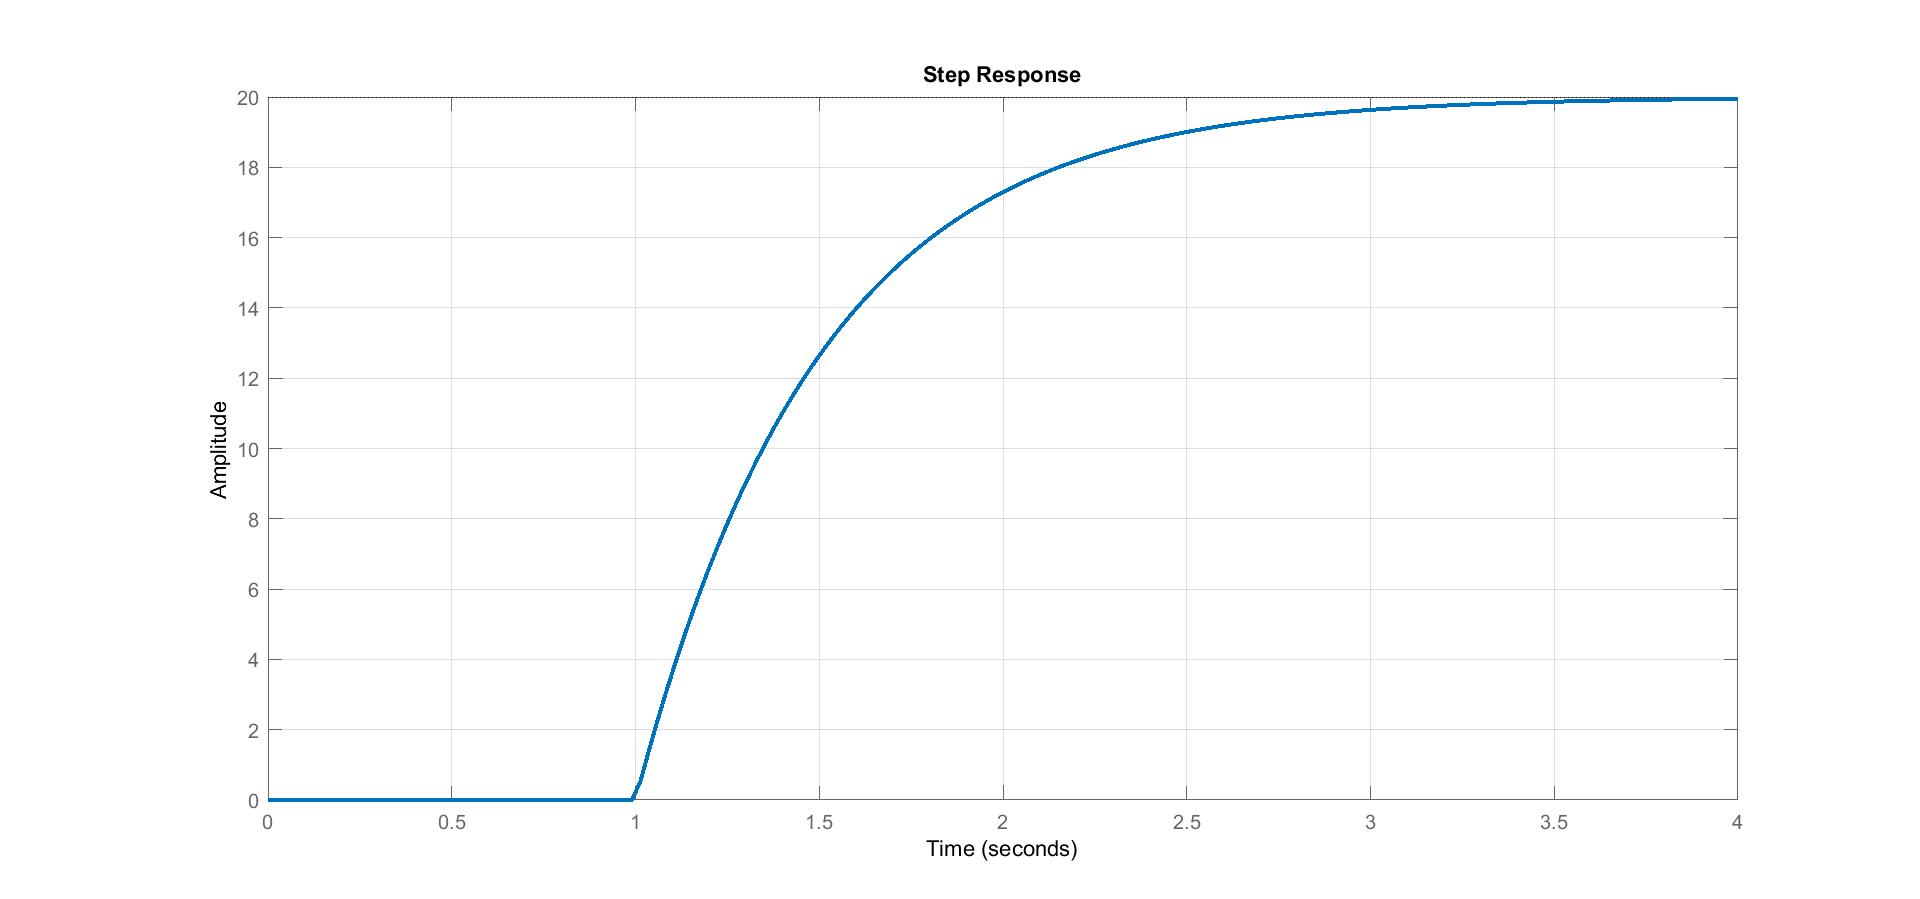
\includegraphics[width=0.75\linewidth]{figs/3.20.jpg}
    \caption{Step response of G(s)}
    \label{fig:prb45}
\end{figure}

\clearpage
\subsection{Step Response}

Consider the transfer function:
\[
G(s)=\frac{1}{s^2+s+1}
\]
Which of the following is the corresponding step response? Explain your choice and why you rejected the other two possibilities.

\begin{figure}[h!]
    \centering
    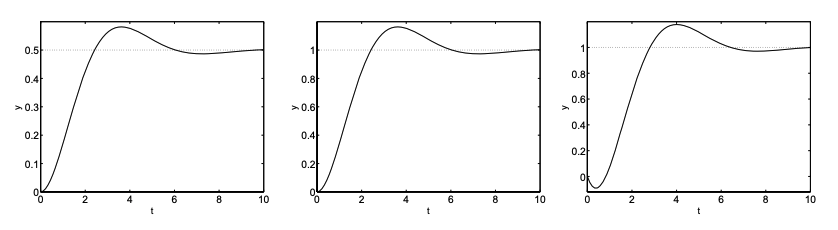
\includegraphics[width=1\linewidth]{figs/3.21.png}
    \caption{Sample step response plots}
    \label{fig:prb50}
\end{figure}
\textbf{\textcolor{red}{Solution :}} \\
The DC gain of H(s) equals 1, so the left plot is immediately rejected because it corresponds to DC gain of 0.5. The right plot show the correct DC gain, but it has an initial dip which indicates the presence of a RHP zero, while H(s) has no zeros. The middle plot is consistent with a stable second-order transfer function with DC gain of 1 and with no zeros, so it is the correct one.

\clearpage
\section{Block Diagrams}
\subsection{Design Pre-Compensators}

Consider a feedback system in the below figure with $G(s) = \frac{2}{s+2}$ and $K(s) = \frac{3s + 12.5}{s}$.
\begin{figure}[h]
    \centering
    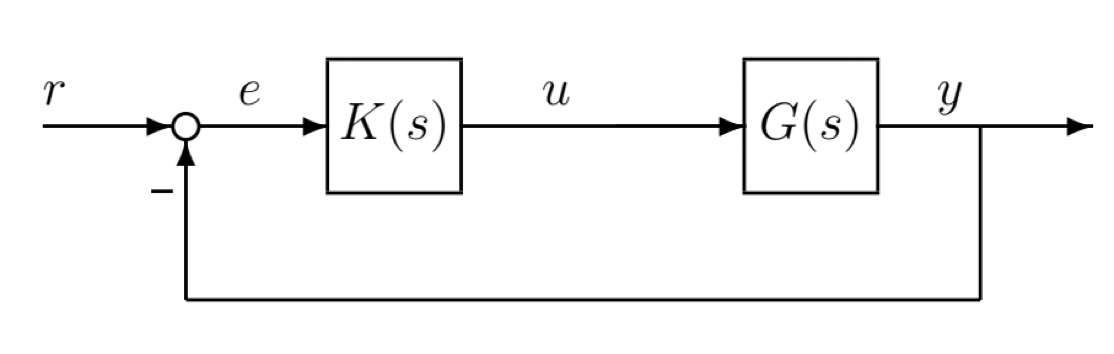
\includegraphics[width=0.7\textwidth]{figs/4.1.png}
    \caption{Standard Feedback System}
    \label{fig:4.1}
\end{figure}
\begin{itemize}
    \item[(a)]  What is the transfer function $T(s)$ from $r$ to $y$?
    \item[(b)] Design a low pass $F(s)$ to filter the reference command.
\end{itemize}

\textbf{\textcolor{red}{Solution :}}

\begin{itemize}
    \item[(a)] $T(s) = \frac{G(s)K(s)}{1+G(s)K(s)} = \frac{6s + 25}{s^2 + 8s + 25}$.
    \item[(b)] Ensuring that $F(0) = 1$, we set $F(s) = \frac{25}{6s+25}$. The resulting closed-loop from $r\rightarrow y$ is now $T(s)F(s) = \frac{25}{s^2+8s+25}$.
\end{itemize}

\clearpage
\subsection{Feedback System Design for Error Specifications}

Consider the general feedback system in the below figure.
\begin{figure}[h]
    \centering
    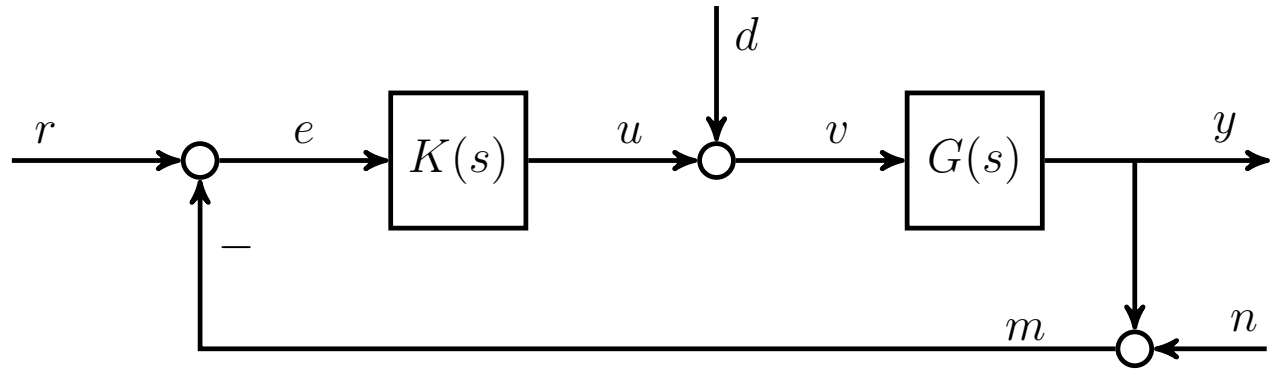
\includegraphics[width=0.7\textwidth]{figs/4.2.png}
    \caption{Standard Feedback System}
    \label{fig:loop_97}
\end{figure}

\begin{itemize}
    \item[(a)] The closed-loop should have zero steady-state error for step reference commands. Translate this into a requirement on the sensitivity $S(s)$. What does this imply about the $L(s)=G(s)K(s)$?
    \item[(b)] The closed-loop should have an error $\leq 0.1$ for reference commands $r(t) = 2\sin(\omega t)$ with $\omega \leq 10$ rad/sec. Translate this into a requirement on the sensitivity $S(s)$.
    \item[(c)] The closed-loop should have an error $\leq 0.05$ for noise $n(t)=10\sin(\omega t)$ with $\omega \geq 1000$ rad/sec. Translate this into a requirement on the complementary sensitivity $T(s)$. 
\end{itemize}

\textbf{\textcolor{red}{Solution :}}

\begin{itemize}
    \item[(a)] Since $S(s) = \frac{1}{1+L(s)}$ and we desire that $S(0)=0$, then we must have $L(0) = +\infty$. $L(s)$ must have a pole at $s=0$.
    \item[(b)] $e(t) \rightarrow 2 |S(j \omega)| \sin(\omega t + \measuredangle S(j \omega)) \leq 0.1$ implies that $|S(j \omega)| \leq 0.05$ for $\omega \leq 10$.
    \item[(c)] $y(t) \rightarrow - 10 |T(j \omega)| \sin(\omega t + \measuredangle T(j\omega)) \leq 0.05$ implies that $|T(j \omega)| \leq 0.05/10 = 0.005$ for $\omega \geq 1000$.
\end{itemize}

\clearpage
\subsection{Overshoot Constraints on Proportional Gains}
For the feedback system shown below determine the range of proportional gains K so that the overshoot of the closed-loop system (in response to the unit step reference input) is no more than $10\%$. \\

\begin{figure}[h!]
    \centering
    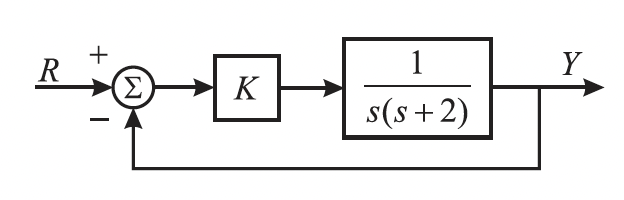
\includegraphics[width=0.8\linewidth]{figs/4.3.png}
    \caption{Standard Feedback System}
    \label{fig:prb36}
\end{figure}
\textbf{\textcolor{red}{Solution :}} \\

\noindent The closed loop transfer function from $R$ to $Y$ is given by:
\[
T(s)=\frac{K}{s^2 + 2s + K}
\]
$\implies \omega_n^2=K, \quad \zeta=\frac{1}{\sqrt{K}} $ or $K=\frac{1}{\zeta^2}$.\\
$M_p \leq 10\% \implies \zeta \geq 0.59$. Therefore, $0 \leq  K \leq 2.86$

\clearpage

\subsection{Tracking a Ramp Reference}
The plant transfer function $G_p(s) = \frac{1}{s^2}$ shown below describes the angle of a pendulum without damping.
\begin{figure}[h!]
    \centering
    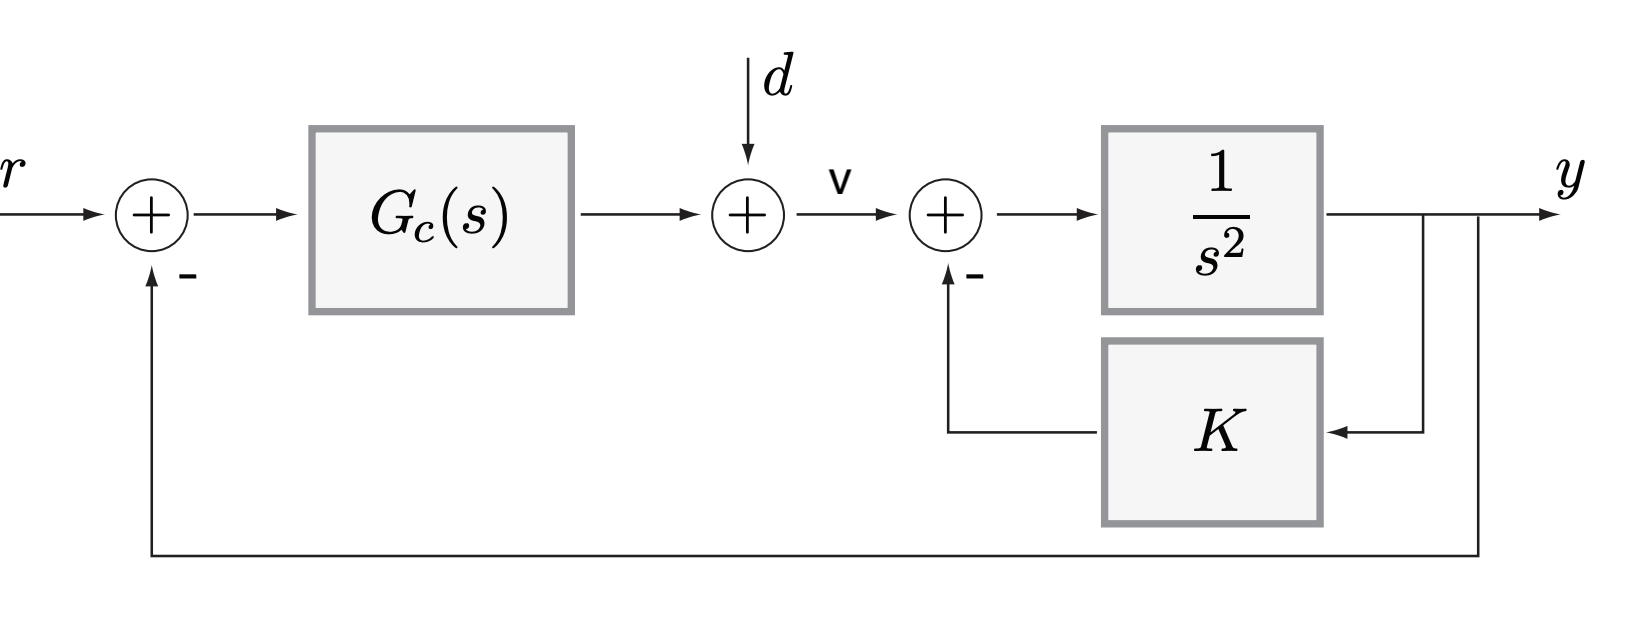
\includegraphics[width=0.75\linewidth]{figs/4.4.png}
    \caption{Representation of an Undamped Pendulum Dynamics}
    \label{fig:prb39}
\end{figure}
\begin{itemize}
    \item [(a)] What conditions must $G_c$ satisfy to ensure that the system can track a ramp reference input with finite steady-state error?
    \item[(b)] Find a compensator that satisfies the conditions of (a). What class of disturbances d(t) will the system reject perfectly?
\end{itemize}
\textbf{\textcolor{red}{Solution :}} \\
\begin{itemize}
    \item [(a)] The plant transfer function $G_p$ is given by:
    \[
    G_p(s)=\frac{Y}{V}=\frac{1}{s^2+K}
    \]
Let $G=G_c(s)G_p(s)$ then with $e=r-y$, we have $ \frac{E}{R}=\frac{1}{1+G}$.


Since $r(t)=t \implies R(s)=\frac{1}{s^2}$, the steady state error is given by:
\[
e_\infty=\lim_{s \rightarrow 0} s E(s)=\lim_{s \rightarrow 0} \frac{1}{s (1+G(s))}
\]
Therefore, $G_c(s)$ must have an integrator controller and we can choose a PID controller.
    \item[(b)] We can try a PID controller with $G_c(s)=K_p + \frac{K_i}{s} + K_d s$. The closed-loop transfer function $\frac{Y}{d}$ is given by:
    \[
    \frac{Y}{d}=\frac{G_p}{1+G} = \frac{s}{s^3+K_d s^2+ (K+K_p) s+K_i}
    \]
    In order to place all the poles at -1, we set $K_i=1$, $K_p=3-K$ and $K_d=3$. This PID compensator will perfectly reject DC disturbances. 
\end{itemize}

\clearpage
\subsection{Stability Analysis}

Consider two systems in a negative feedback configuration shown below:
\begin{figure}[h!]
    \centering
    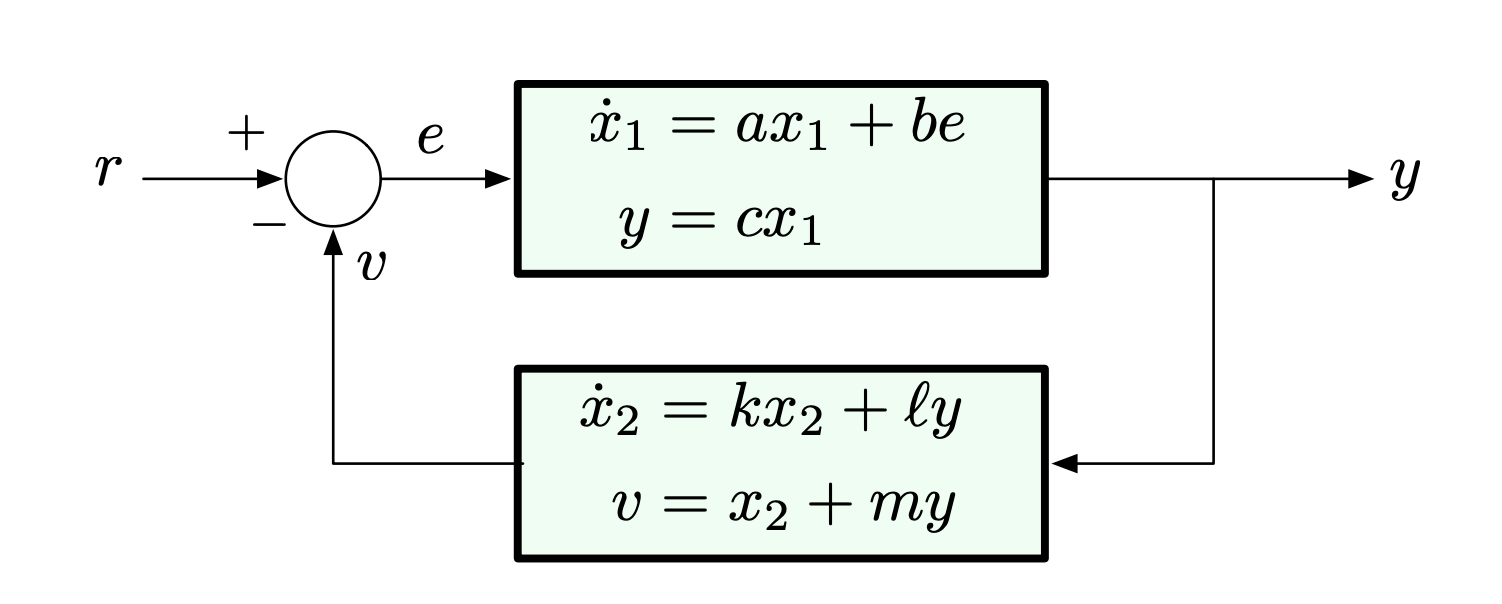
\includegraphics[width=0.75\linewidth]{figs/4.5.png}
    \caption{Negative Feedback Configuration}
    \label{fig:enter-label}
\end{figure}


Write down the conditions that must be satisfied by the system parameters
a, b, c, k, l, m for this transfer function to be stable (i.e., for all poles to have
negative real parts). \\
\textbf{\textcolor{red}{Solution :}} \\
Notice that the denominator of the transfer function is a monic second order polynomial in the form $p(s)=s^{2}+a_{1} s+a_{2} $


In order for the system to be stable, we need all roots of (5) to be in the OLHP. When the determinant of (5) is non-negative, that is, $a_{1}^{2}-4 a_{2} \geq 0$, we need both roots to be negative:

$$
\frac{-a_{1} \pm \sqrt{a_{1}^{2}-4 a_{2}}}{2}<0 \Rightarrow a_{1}>0,0<a_{2} \leq \frac{a_{1}^{2}}{4}
$$

When $a_{1}^{2}-4 a_{2}<0$, we need the real part of the roots to be negative:

$$
\frac{-a_{1}}{2}<0 \Rightarrow a_{1}>0, a_{2}>\frac{a_{1}^{2}}{4}
$$

Hence it can be summarized that we need both $a_{1}>0, a_{2}>0$ in order for the system to be stable. This condition can be directly obtained by using Routh-Hurwitz criterion. Substitute $a_{1}, a_{2}$ with the system parameters given, all we need is:

$$
\left\{\begin{aligned}
& b c m-a-k>0 \\
& a k+b c l-b c k m>0
\end{aligned}\right.
$$

\clearpage
\section{Control System Design}

\subsection{PI Control Design}
Consider a plant with a nominal model given by
\begin{equation}
G(s) = \frac{1}{s + 2}
\end{equation}
Compute the parameters \(K_p\) and \(K_i\) of a PI controller so that the natural modes of the closed loop response decay as fast as \(e^{-5t}\). 

\textbf{\textcolor{red}{Solution :}}
% Short Answer: For a decay rate as fast as \(e^{-5t}\), \(K_p = 8\) and \(K_i \geq 25\).
% Reasoning Steps:
A PI controller has a transfer function given by
\begin{equation}
C(s) = \frac{K_ps + K_i}{s};
\end{equation}
The closed-loop characteristic polynomial, \(A_{cl}(s)\), is derived as
\begin{equation}
A_{cl}(s) = \text{numerator of } \{1 + G(s)C(s)\} = s^2 + (2 + K_p)s + K_i.
\end{equation}
To achieve a closed-loop transient response that decays as fast as \(e^{-5t}\), the controller must generate a pair of complex conjugate poles with real parts equal to \(-5\). This requirement determines the values of \(K_p\) and \(K_i\), with \(K_p\) needing to be 8 and \(K_i\) needing to be greater than or equal to 25. Therefore, the appropriate PI controller parameters are \(K_p = 8\) and \(K_i \geq 25\).
% Problem End

\clearpage
\subsection{Pole Assignment}

A plant with nominal model 
\begin{equation}
    G_o(s) = \frac{1}{(s + 1)^2}
\end{equation}
is in a feedback loop under control with a PI controller having transfer function $C(s) = \frac{K_ps + K_i}{s}$.
Determine whether this controller configuration can be used to achieve full pole placement.

\textbf{\textcolor{red}{Solution :}} \\ 
The plant is of second-order, and the controller introduces an additional third pole. However, the controller only have two gains, corresponding to two numerator coefficients, which generally precludes it from being used to place all three poles effectively.
\clearpage
\subsection{Minimal-Order Control Design}

Consider a nominal model for a plant given by:
\begin{equation}
G_o(s) = \frac{B_o(s)}{A_o(s)}=\frac{1}{(s + 1)(s - 2)}
\end{equation}
The closed-loop characteristic polynomial is defined as:
\begin{equation}
A_{cl}(s) = (s + 2)(s + 3)(s + 4)(s + 5)
\end{equation}
Design a controller \(C(s)\) that satisfies the following conditions:\\
- Results in the given closed-loop characteristic polynomial.\\
- Has the minimum order numerator to ensure system stability.\\
- Express both the numerator and the denominator of \(C(s)\) as expanded polynomials.\\

Provide the transfer function of the designed controller in the format: " \(C(s) = \frac{P(s)}{L(s)}=\frac{Numerator}{Denominator}\)", where Numerator and Denominator are fully expanded polynomials.

\textbf{\textcolor{red}{Solution :}} \\ 
% Short Answer: \(C(s) = \frac{272s + 296}{s^2 + 15s + 88}\)
% Reasoning Steps:
The degree of $A_{cl}(s)$ is four and the degree of $A_o(s)$ is two. Hence $L(s)$ should have a degree equal to two. Then
\begin{equation}
C(s) = \frac{p_2s^2 + p_1s + p_0}{s^2 + \lambda_1s + \lambda_0}
\end{equation}
The corresponding pole assignment equation becomes
\begin{equation}
A_o(s)L(s) + B_o(s)P(s) = (s + 2)(s + 3)(s + 4)(s + 5)
\end{equation}
\begin{equation}
(s + 1)(s - 2)(s^2 + \lambda_1s + \lambda_0) + (p_2s^2 + p_1s + p_0) = (s + 2)(s + 3)(s + 4)(s + 5)
\end{equation}
\begin{equation}
s^4 + (\lambda_1 - 1)s^3 + (p_2 - \lambda_1 + \lambda_0 - 2)s^2 + (p_1 - \lambda_0 - 2\lambda_1)s + (p_0 - 2\lambda_0) = s^4 + 14s^3 + 71s^2 + 154s + 120
\end{equation}
This polynomial identity leads to the equations
\begin{align}
\lambda_1 - 1 &= 14 \\
p_2 - \lambda_1 + \lambda_0 - 2 &= 71 \\
p_1 - \lambda_0 - 2\lambda_1 &= 154 \\
p_0 - 2\lambda_0 &= 120
\end{align}
The solution of these equations is
\begin{align}
\lambda_1 &= 15 \\
p_2 &= 73 + \lambda_1 - \lambda_0 = 88 - \lambda_0 \\
p_1 &= 154 + 2\lambda_1 + \lambda_0 = 184 + \lambda_0 \\
p_0 &= 120 + 2\lambda_0
\end{align}
We thus observe that there is an infinite number of solutions. Every choice of $\lambda_0$ leads to a different stabilizing controller, for example, to force integration in the controller we can choose $\lambda_0 = 0$
\begin{equation}
C(s) = \frac{88s^2 + 184s + 120}{s^2 + 15s}
\end{equation}
In MATLAB we can solve this problem with the command line
\begin{verbatim}
>> [L,P]=paq([1 -1 -2],1,[1 14 71 154 120])
\end{verbatim}
This leads to
\begin{equation}
C(s) = \frac{272s + 296}{s^2 + 15s + 88}
\end{equation}
This is equivalent to choosing $\lambda_0 = 88$. The algorithm in \texttt{paq.m} has been designed to yield a minimum degree $P(s)$.
% Problem End 

\clearpage
\subsection{Pole Placement}

Consider a nominal model given by:
\begin{equation}
G_o(s) = \frac{3s + 1}{(s + 2)(s - 3)}
\end{equation}
The goal is to design a control law that tracks a constant reference and cancels the pole at \(s = -2\) in \(G_o(s)\). Design a suitable controller. If pole placement is required for the characteristic equation, start with a pole at \(s = -2\) and for any additional poles required, increase their magnitude sequentially (e.g., for three required poles, assign them at \(-2\), \(-3\), and \(-4\); and so forth). Provide the transfer function of the designed controller in the format: " \(C(s) = \frac{Numerator}{Denominator}\)", where Numerator and Denominator are fully expanded polynomials.

\textbf{\textcolor{red}{Solution :}} \\ 
% Short Answer: \(C(s) = \frac{-44s^2+212s + 600}{5s^2 + 207s}\)
% Reasoning Steps:
The minimum degree of $A_{cl}(s)$ is four since we need to force integration in the controller, then
\begin{equation}
C(s) = \frac{p_2s^2 + p_1s + p_0}{s(s + \lambda_1)}
\end{equation}
Since $(s + 2)$ is cancelled if and only if $(s + 2)$ is a factor of $A_{cl}(s)$, we choose
\begin{equation}
A_{cl}(s) = (s + 2)(s + 3)(s + 4)(s + 5)
\end{equation}
The pole assignment equation then becomes
\begin{equation}
A_o(s)L(s) + B_o(s)P(s) = (s + 2)(s + 3)(s + 4)(s + 5)
\end{equation}
\begin{equation}
(s + 2)(s - 3)(s + \lambda_1)s + (3s + 1)(p_2s^2 + p_1s + p_0) = (s + 2)(s + 3)(s + 4)(s + 5)
\end{equation}
In this polynomial identity we note that $(s + 2)$ has to be a factor of $P(s)$ (a plant pole can only be cancelled by a controller zero). Thus we define
\begin{equation}
(s + 2)(\tilde{p}_1s + \tilde{p}_0) = p_2s^2 + p_1s + p_0
\end{equation}
The pole assignment equation then simplifies as follows:
\begin{equation}
(s - 3)(s + \lambda_1)s + (3s + 1)(\tilde{p}_1s + \tilde{p}_0) = (s + 3)(s + 4)(s + 5)
\end{equation}
\begin{equation}
s^3 + (3\tilde{p}_1 + \lambda_1 - 3)s^2 + (\tilde{p}_1 + 3\tilde{p}_0 - 3\lambda_1)s + \tilde{p}_0 = s^3 + 12s^2 + 47s + 60
\end{equation}
This leads to equations
\begin{align}
3\tilde{p}_1 + \lambda_1 - 3 &= 12 \\
\tilde{p}_1 + 3\tilde{p}_0 - 3\lambda_1 &= 47 \\
\tilde{p}_0 &= 60
\end{align}
The solution is $\tilde{p}_0 = 60$, $\tilde{p}_1 = -\frac{44}{5}$ and $\lambda_1 = \frac{207}{5}$. Finally the controller is
\begin{equation}
C(s) = \frac{(s + 2)(-44s + 300)}{s(5s + 207)}
\end{equation}
% Problem End

\clearpage
\subsection{Proportional Controller}

Answer True or False to the following questions. Also justify your answers.
\begin{itemize}
    \item[(a)] Let \(y(t)\) be the response of an LTI system \(G(s)\) with zero initial conditions due to the input \(u(t)\). The response of \(G(s)\) with nonzero initial conditions and input \(2*u(t)\) will always be equal to \(2*y(t)\).
    \item[(b)] An LTI system \(G(s)\) with a zero in the right half plane will always have an unbounded step response.
    \item[(c)] Let \(G(s)\) be an LTI system with one real pole that has a time constant five times larger than all the other poles. A dominant pole approximation for \(G(s)\) will be reasonably accurate.
    \item[(d)]Let \(G(s)\) be a second-order LTI system and \(K(s)\) be a PID controller designed to place all closed-loop poles in the left half plane. If the derivative term is implemented using an approximate derivative then the resulting closed-loop will be fourth order.
    \item[(e)] Consider a control system with the plant \(G(s) = \frac{5}{s^2+s}\) and a proportional controller with gain \(k_p\). It is possible to choose \(k_p\) so that the closed-loop is stable and has zero steady-state error due to a unit step reference command.
\end{itemize}
\textbf{\textcolor{red}{Solution :}} \\
\begin{itemize}
    \item[(a)] False
    \item[(b)] False
    \item[(c)] True
    \item[(d)] True
    \item[(e)] True
\end{itemize}

\clearpage
\subsection{PI Controller}

Consider a feedback system with the plant and controller:
$$G(s) = \frac{2}{s+2}, \qquad K(s) = \frac{s+0.5}{s}.$$

 What type of controller has the transfer function $K(s)$?

\textbf{\textcolor{red}{Solution :}} \\
$K(s)$ is a PI controller with $K_p = 1$ and $K_i = 0.5$.

\clearpage
\subsection{Proportional Controller}

Consider the following plant:
\begin{equation}
    \ddot{y}(t) + 2 \dot{y}(t) + 10 y(t) = 20 u(t) + 10 d(t)
\end{equation}
\begin{itemize}
    \item[(a)] What is the model from inputs \((r,d)\) to output \(y\) if we use an open-loop controller \(u(t) = K_{ol}r(t)\)?
    \item[(b)] Can the gain \(K_{ol}\) be selected so that the control system is overdamped from \(r\) to \(y\)?
    \item[(c)] Select \(K_{ol}\) so that \(y(t) \rightarrow \bar{r}\) when \(r(t) = \bar{r}\) and \(d(t) = 0\)
    \item[(d)] What is the impact of the disturbance \(d(t)\) when \(r(t) = 2\) and \(d(t) = 1\)
\end{itemize}
\textbf{\textcolor{red}{Solution :}} 
\begin{itemize}
    \item[(a)] $ \ddot{y}(t) + 2 \dot{y}(t) + 10 y(t) = 20 K_{ol}r(t) + 10 d(t)$
    \item[(b)] No, it is underdamped for any choice of \(K_{ol}\).
    \item[(c)] Set \(\ddot{\bar{y}} = \dot{\bar{y}} = 0 \rightarrow 10 \bar{y} = 20 K_{ol} \bar{r}\), thus \(K_{ol} = \frac{1}{2}\)
    \item[(d)] It causes error in steady state solution.
\end{itemize}

\clearpage
\subsection{Proportional Controller}

Consider the following plant:
\begin{equation}
    2\dot{y}(t) + 3 y(t) = -4 u(t) + d(t)
\end{equation}
\begin{itemize}
    \item[(a)] What is the model from inputs \((r,d)\) to output \(y\) if we use an proportional controller \(u(t) = K_p (r(t)-y(t))\)?
    \item[(b)] Select \(K_p\) so that the steady-state error \(\bar{e} = \bar{r} - \bar{y}\) is less than \(0.1\) when \(r(t) = \bar{r} = 2\) and \(d(t) = \bar{d} = 1\).
    \item[(c)] What is the time constant of the closed-loop?
\end{itemize}
\textbf{\textcolor{red}{Solution :}} 
\begin{itemize}
    \item[(a)] $ 2 \dot{y}(t) + (3-4 K_p) y(t) = -4 K_p r(t) + d(t)$
    \item[(b)] The closed-loop is stable if and only if \(K_p < \frac{3}{4}\). Also, in steady-state we have:
    \begin{align}
        \bar{e} = \bar{r} - \bar{y} &= \left(1+\frac{4 K_p}{3-4K_p} \right)\bar{r} - \frac{1}{3-4K_p} \bar{d} \\ &= \left(1+\frac{4 K_p}{3-4K_p} \right)2 - \frac{1}{3-4K_p} 1 \\
        & = 2 + \frac{8K_p-1}{3-4K_p} < 0.1
    \end{align}
    Thus,
    \begin{equation}
        K_p < -11.75
    \end{equation}
    \item[(c)] \(\tau = \frac{2}{3-4K_p}\)
\end{itemize}

\clearpage
\subsection{PI Controller}

Consider the following plant:
\begin{equation}
    2\dot{y}(t) + 6y(t) = 8 u(t)
\end{equation}
with a PI controller in the following form:
\begin{equation}
    u(t) = K_p e(t) + K_i \int_0^t e(\tau) d\tau
\end{equation}
where \(e(t) = r(t) - y(t)\)
\begin{itemize}
    \item[(a)] What is the ODE model for the closed-loop from \(r(t)\) to \(y(t)\)?
    \item[(b)] Choose \((K_p,K_i)\) so that the closed-loop :
    \item Stable
    \item Settling time \(t_s = \frac{3}{\zeta \omega_n}\) is \(3\)
    \item damping ratio \(\zeta = 0.5\)
    \item[(c)] How will rising time, overshoot and settling time change if \(K_i\) is increased further?
\end{itemize}
\textbf{\textcolor{red}{Solution :}} 
\begin{itemize}
    \item[(a)] \(2\ddot{y}(t) + (6 + 8 K_p) \dot{y}(t) + 8 K_i y(t) = 8 K_p \dot{r}(t) + 8 K_i r(t) \)
    \item[(b)] \(\zeta \omega_n = 1 \quad \text{and} \quad \zeta = 0.5 \rightarrow \omega_n = 2\) \\
    Thus,
    \begin{equation}
        K_p = - \frac{1}{4} \quad K_i = 1
    \end{equation}
    \item[(c)] \(2\zeta \omega_n\) remains unchanged and \(\omega_n\) increases.
    Increasing \(K_i\) makes the following change:
    \begin{itemize}
        \item rising time \(\uparrow\)
        \item overshoot \(\downarrow\)
        \item settling time, does not change
    \end{itemize}
\end{itemize}

\clearpage
\subsection{PD Controller}

Consider the following plant:
\begin{equation}
    \ddot{y}(t) - 2\dot{y}(t) + y(t) = u(t)
\end{equation}
with a PD controller in the following form:
\begin{equation}
    u(t) = K_p(r(t)-y(t))-K_d \dot{y}(t)
\end{equation}
\begin{itemize}
    \item[(a)] What is the ODE model for the closd-loop from \(r(t)\) to \(y(t)\)?
    \item[(b)] Choose \((K_p,K_d)\) so that the closed-loop is: 
    \item stable
    \item has \((\omega_n,\zeta)\) = (2rad/sec,0.5)
    \item[(c)] What is the steady-state error if \(r\) is a unit step reference?
    \item[(d)] Would you increase or decrease \(K_p\) to reduce the steady-state error?
\end{itemize}
\textbf{\textcolor{red}{Solution :}} 
\begin{itemize}
    \item[(a)] \(\ddot{y}(t) + (K_d-2) \dot{y}(t) + (K_p+1)y(t) = K_p r(t)\)
    \item[(b)] \(K_p = 3\) and \(K_d = 4\)
    \item[(c)] \(4 \bar{y} = 3 \bar{r} = 3 \rightarrow \bar{y} = \frac{3}{4}\) \\
    Thus,
    \begin{equation}
        \bar{e} = \bar{r} - \bar{y} = \frac{1}{4}
    \end{equation}
    \item[(d)] \(\bar{y} = \frac{K_p}{K_p + 1} \bar{r}\).
    Thus, increasing \(K_p\) reduce steady-state error.
\end{itemize}

\clearpage
\subsection{PID Controller}

Consider the plant with the following transfer function:
\begin{align*}
    G(s) = \frac{505}{s^3+21s^2+121s+101}
\end{align*}
The poles of this system are at \(s = -1, -10 \pm j\), and  and the DC gain is $5$.
\begin{itemize}
    \item[(a)] What is the dominant pole approximation \(G_a(s)\) for this plant?
    \item[(b)] Would you recommend using a PI, PD, or PID controller?
    \item[(c)] Choose the controller gains so that the closed-loop with \(G_a(s)\) has poles repeated at \(s = -1\)
\end{itemize}
\textbf{\textcolor{red}{Solution :}} 
\begin{itemize}
    \item[(a)] Set \(G_a(s) = \frac{b_0}{s+1}\). Since \(G(0) = \frac{505}{101}\), we have \(b_0 = 5\). Thus,
\begin{equation}
    G_a(s) = \frac{5}{s+1}
\end{equation}
The time-domain approximation of \(G_a(s)\) is:
\begin{equation}
    \dot{y}(t) + y(t) = 5 u(t)
\end{equation}
    \item[(b)]  PI controller
    \item[(c)] Desired characteristic equation:
    \[ (s+1)^2 = 0\]\
    Using the following PI controller:
    \[u(t) = K_p (r(t)-y(t)) + K_i \int (r(t)-y(t))\]
    we have:
    \[\ddot{y}(t) + (1+5K_p)\dot{y}(t) + 5K_i y(t) = 5K_p \dot{r}(t) + 5K_i r(t)\]
    Thus:
    \(K_p = 0.2\) and \(K_i = 0.2\)
\end{itemize}

\clearpage
\subsection{PI Controller}

Consider the plant with the following transfer function:
\begin{equation}
    G(s) = \frac{505}{s^3+21s^2+121s+101}
\end{equation}
The poles of this system are at \(s = -1, -10 \pm j\).
\begin{itemize}
    \item[(a)] What is the dominant pole approximation \(G_a(s)\) for this plant?
    \item[(b)] Choose the controller gains so that the closed-loop with \(G(s)\) has poles repeated at \(s = -2\)
\end{itemize}
\textbf{\textcolor{red}{Solution :}} 
\begin{itemize}
    \item[(a)] Set \(G_a(s) = \frac{b_0}{s+1}\). Since \(G(0) = \frac{505}{101}\), we have \(b_0 = 5\). Thus,
\begin{equation}
    G_a(s) = \frac{5}{s+1}
\end{equation}
The time-domain approximation of \(G_a(s)\) is:
\begin{equation}
    \dot{y}(t) + y(t) = 5 u(t)
\end{equation}
\item[(b)]  Desired characteristic equation:
    \[ (s+2)^2 = 0\]\
    Using the following PI controller:
    \[u(t) = K_p (r(t)-y(t)) + K_i \int (r(t)-y(t))\]
    we have:
    \[\ddot{y}(t) + (1+5K_p)\dot{y}(t) + 5K_i y(t) = 5K_p \dot{r}(t) + 5K_i r(t)\]
    Thus:
    \(K_p = 0.6\) and \(K_i = 0.8\)
\end{itemize}

\clearpage
\subsection{PID Controller}

Consider the plant with the following transfer function:
\begin{equation}
    G(s) = \frac{20}{s^2-6s+10}
\end{equation}
\begin{itemize}
    \item[(a)] What is the closed-loop ODE from reference \(r\) to output \(y\) if we use the following PID controller?
    \[u(t) = K_p e(t) + K_i \int e(t) + K_d \dot{e}(t)\]
    where \(e(t) = r(t) - y(t)\)
    \item[(b)] Choose the controller gains so that the closed-loop has poles repeated at \(s = -3\). Hint: \((s+3)^3 = s^3+9s^2+27s+27\)
    \item[(c)] What is the impact of the implementing the derivative term \(K_d \dot{e}(t)\) as versus the rate feedback from \(-K_d \dot{y}(t)\)?
\end{itemize}
\textbf{\textcolor{red}{Solution :}} 
\begin{itemize}
    \item[(a)] \(G(s)\) in the time-domain can be written as
    \[\ddot{y}(t) - 6\dot{y}(t) + 10 y(t) = 20 u(t)\]
    using the PID controller \(u(t)\), we have:
    \[\dddot{y}(t) + (20 K_d-6)\ddot{y}(t) + (10 + 20 K_p)\dot{y}(t) + 20 K_i y(t) = 20 K_d \ddot{r}(t) + 20 K_p \dot{r}(t) + 20 K_i r(t)\]
    \item[(b)]
    we have:
    \[K_p =\frac{17}{20}, K_i = \frac{27}{20}, K_d = \frac{15}{20}\]
    \item[(c)] \(K_d \dot{e}(t)\) causes an extra term in the numerator of the transfer function (extra zero). If \(\dot{r}(t)\) changes fast, this causes overshoot/oscillatory.
\end{itemize}

\clearpage
\subsection{PI Controller}

Consider the following plant and PI controller:
\[2\dot{y}(t) + 6y(t) = 8u(t) \quad \quad  u(t) = 2.5e(t) + 9 \int_0^t e(\tau) d\tau\]
\begin{itemize}
    \item[(a)] What sampling time \(\Delta t\) would you recommend for a discrete-time implementation?
    \item[(b)] The value of \(u(t)\) at \(t = \Delta t\) is:
    \[u(\Delta t) = 2.5e(\Delta t) + 9 \int_0^{\Delta t} e(\tau) d\tau \]
    Approximate \(u_1:= u(\Delta t)\) in terms \(e_0 := e(0)\) and \(e_1:=e(\Delta t)\).

\end{itemize}
\textbf{\textcolor{red}{Solution :}}
\begin{itemize}
    \item[(a)]
    \[2\ddot{y}(t) + 26 \dot{y}(t) + 72 y(t) = 20 \dot{r}(t) + 72 r(t)\]
    Thus,
    \[T_{r \rightarrow y}(s) = \frac{20s+72}{2s^2 + 26s + 72}\]
    The poles of the transfer function are \(s_1 = -4\) and \(s_2 = -9\). The corresponding time constants are \(\tau_1 = \frac{1}{4}\) and \(\tau  = \frac{1}{9}\).
    One good approximation for \(\Delta t\) would be
    \[\Delta t = \frac{1/9}{10} \approx \frac{1}{100} = 10 \text{msec}\]
    \item[(b)] Using this approximation \(\int_0^{\Delta t} e(\tau) d\tau \approx \frac{1}{2}(e_0 + e_1) \Delta t\), we have:
    \[u_1 \approx  2.5 e_1 + 9(\frac{1}{2}(e_0 + e_1) \Delta t)\]
\end{itemize}
\clearpage

\subsection{Proportional Controller}

Consider the transfer function
\begin{equation}
    T(s) = \frac{b_0 K_p}{s^2+a_1s+(a_0 + b_0 K_p)}
\end{equation}
where \(b_0 > 0\) and the closed-loop is critically damped. What happens to the settling time if \(K_p\) is increased? \(K_p\) is decreased?

\textbf{\textcolor{red}{Solution :}} \\
We have \(a_1 = 2\zeta \omega_n\) and \(a_0 + b_0 K_p = 2  \omega_n^2\). \\
\begin{itemize}
    \item Increasing \(K_p\) does not change the real part and thus settling time \(t_s\) remain unchanged.
    \item Decreasing \(K_p\) brings one of the poles closer to the origin, thereby increasing the settling time \(t_s\).
\end{itemize}
\clearpage

\subsection{PI Controller}

Consider a car whose longitudinal motion is modeled by the following ODE:
$$2085 \dot{v}(t) + 23.2v(t) = 40u(t) + 108.4 - F_{grav}(t)$$
The input is the throttle u and the output is the velocity v. The gravitational force $F_{grav}$ is a disturbance. Let $e(t) = v_{des}- v(t)$ denote the tracking error between the desired velocity $v_{des} = 29$ m/s and actual velocity v(t). Consider a PI controller of the following form:
$$ u(t) =  \bar{u} + K_p e(t) + K_i \int_0^t  e(\tau) d\tau  $$
where $\bar{u}=14.11$ is the open-loop input to maintain $v_{des}$ when on 
at road $\theta= 0^\circ$ . Choose the PI gains so that the cruise control system is stable and rejects disturbances due to changing road slopes within $\approx 10$ sec. The closed-loop should also be over or critically damped as oscillations are uncomfortable for the driver. \\
\textbf{\textcolor{red}{Solution :}} \\
This particular problem is of interest as it is one of the first design problems encountered by undergraduate control engineer. Moreover, it requires reasoning about the impact of the control gains on the closed-loop poles and the connection to transient response properties. There is more than one design that satisfies the given objectives.  One approach is to note that the closed-loop characteristic equation is:
\begin{align*}
 2085 s^2 + (23.2 + 40K_p) s + 40K_i =0
\end{align*}
We can place the closed-loop poles in the LHP to have any desired damping ratio $\zeta$ and natural frequency $\omega_n$ by choosing the controller gains to satisfy $\omega_n^2 = \frac{40K_i}{2085}$
and $2\zeta\omega_n = \frac{23.2+40K_p}{2085}$.  Select $\zeta=1$ to obtain two critically damped closed-loop poles placed at $s=-\omega_n$. The time constant for these poles is $\tau=\frac{1}{\omega_n}$ sec and, for critically damped poles, the 5\% settling time is approximately $4.75\tau = \frac{4.75}{\omega_n}$.  Thus we select $\omega_n = \frac{4.75}{10} = 0.475$ to obtain a settling time near 10sec.  Finally, use $\zeta=1$ and $\omega_n=0.475$ to solve for the PI gains using the relations above. This yields $K_p=48.94$ and $K_i=11.76$.  The corresponding transfer function from $F_{grav}$ to $v$ is
\begin{align*}
    T_{Fgrav \to v}(s) = \frac{-s}{2085 s^2 + 1981 s + 470.4}
\end{align*}
This has critically damped poles at $s=-0.475$ as expected. A step change increase in gravitational force (due to a step increase in the road slope) will cause the velocity to initially drop from the desired value.  However, the PI controller rejects the disturbance in $\approx 10sec$ with the velocity converging to the desired value with a nice overdamped response.
\clearpage

\subsection{Proportional Controller}

Consider the following first order system:
\[
\dot{y} = -0.5y + 2u \qquad  y(0) = 0
\]
with a proportional control law $u(t) = K_p(r(t) - y(t))$ where $r(t)$ is the reference command. Assume a unit step for $r(t)$. For what gains $K_p$ is $|u(t)| \leq 1$ for all time?\\
\textbf{\textcolor{red}{Solution :}} \\
Note that the magnitude $|u (t)|$ of the control law is directly proportional to the difference
between the state value and the reference value. i.e. $|r(t) - y(t)|$ via the gain $K_p$. Notice that the largest value of $|u(t)|$ will occur at t = 0 which gives us
\[
\max_t |u(t)| =|K_p||r(0)-y(0)|=|K_p||1-0|=|K_p|
\]
Therefore a preliminary condition for $|u(t)| \leq 1$ for all $t \in \mathbb{R}_+$ is that $|u\leq 1|$. However, note that we can write:
\[
\dot{y}=-0.5y +2 u= -y (0.5 + 2K_p) + 2K_p r
\]
and so when $K_p = 0$ we get a stable autonomous system with eigenvalue 0.5. On the
other hand, for any constant reference signal $r(t) \equiv$const we have that $K_p < -0.25$ will result in an unstable system. But note, that by solving for y(t) we see that further we
need,

$$|u (t)| \leq \left| K_p \left( 1- \frac{2 K_p}{0.5 + 2 K_p}\right) \right|\leq 1$$
Therefore, the acceptable range is $K_p \in [-0.2, 1]$.
\clearpage

\subsection{Proportional Controller}

Consider the following first order system:
\[
\dot{y} = -0.5y + 2u \qquad  y(0) = 0
\]
with a proportional control law $u(t) = K_p(r(t) - y(t))$ where $r(t)$ is the reference command. Under the constraint that $K_p \in [-0.2, 1]$, find $K_p$ such that we minimizes the steady-state error due to the unit step reference command. What is the time constant of the closed-loop system for this gain?\\
\textbf{\textcolor{red}{Solution :}} \\
For $K_p \in [-0.2, 1]$ it is clear that steady-state error to a unit-step reference input is
maximized at the left end-point of the interval and minimized at the right end-point. To
see why derive the transfer function:
\[
\frac{Y(s)}{R(s)}=\frac{2 K_p}{s+2 K_p +0.5}
\]
and we see using Final Value Theorem that for higher $K_p$ the steady-state value approaches 1. Hence, we choose $K_p = 1$ to satisfy the constraint. The corresponding transfer function is given as follows:
\[
H(s) =\frac{2}{s+5/2} \qquad \implies \tau=\frac{2}{5}
\]
\clearpage

\subsection{PI Controller}

Consider the following first order system:
\[
\dot{y} = -0.5y + 2u \qquad  y(0) = 0
\]
with a proportional-integral (PI) control law: 
$$u(t)=K_p e(t)+K_i \int_0^t e(\tau) d \tau$$ with $e(t)=r(t)-y(t)$ is the tracking error. Combining the system model and PI controller leads to the closed-loop system in the following form:
\[
\ddot{y}+ a_1 \dot{y} + a_0 y = b_1 \dot{r} + b_0 r
\]
How do the damping ratio and natural frequency depend on $K_p$ and $K_i$? What is the steady state error if $r$ is a unit step? \\
\textbf{\textcolor{red}{Solution :}} \\
The second order system in the above ODE form gives us:
\[
a_0 = 2K_p + 1=2 \qquad  a_1 = 2K_i \qquad b_0 = 2K_i \qquad b_1 = 2K_p
\]
The characteristic polynomial then is:
\[
s^2 + s (2K_p + \frac{1}{2}) + 2K_i \implies \omega_n = \sqrt{2K_i} \quad \text{and} \quad \zeta = \frac{4K_p + 1}{4\sqrt{2K_i}}
\]
For a unit-step reference signal this results in zero steady state error.
\clearpage

\subsection{PI Controller}

Consider the following first order system:
\[
\dot{y} = -0.5y + 2u \qquad  y(0) = 0
\]
with a proportional-integral (PI) control law:  $u(t)=K_p e(t)+K_i \int_0^t e(\tau) d \tau$ with $e(t)=r(t)-y(t)$. Let $K_p=1$ and choose $K_i$ to obtain a damping ratio of $\zeta = 0.7$.  For these PI gains, what are the estimated maximum overshoot and $5\%$ settling time (neglecting the integral effect of the zero)? \\
\textbf{\textcolor{red}{Solution :}} \\
The characteristic polynomial for the system with PI controller is given by:
\[
s^2 + s (2K_p + \frac{1}{2}) + 2K_i \implies \omega_n = \sqrt{2K_i} \quad \text{and} \quad \zeta = \frac{4K_p + 1}{4\sqrt{2K_i}}
\]
Plugging in $K_p = 1$ and $\zeta=0.7$ into the last equation above yields that $K_i =\frac{625}{392}$ and $\omega_n=1.7857$. We know,
\[
M_p=\exp{\left(\frac{-\zeta \pi }{\sqrt{1-\zeta^2}}\right)} \approx 4.6\%
\]
and for $5\%$ settling time,
\[
T_s =\frac{-ln (5/100)}{\zeta \omega_n}=\frac{-ln (.05)}{0.7 \times 1.7857} =2.4s
\]
\clearpage

\subsection{PD Controller}

Consider the following first order system:
\[
\ddot{y} +2\dot{y} +y = u \qquad  y(0) = 0
\]
with a PD controller in the form $u(t) = K_p(r(t) - y(t)) + K_d \dot{y}(t)$.
Choose $(K_p, K_d)$ so that the closed loop system is stable and has $(\omega_n, \zeta) = (2, 0.25)$. \\
\noindent \textbf{\textcolor{red}{Solution :}} \\
We can derive the transfer function as follows:
\begin{equation*}
\begin{split}
H(s) =\frac{Y (s)}{R(s)} &= \frac{K_p}{s^2 + (2 - K_d )s + (K_p + 1)} \\
&= \left( \frac{K_p}{K_p+1}\right)
    \frac{K_p + 1}{s^2 + (2-K_d)s + (K_p + 1)}
\end{split}
\end{equation*}
So, $\omega^2_n = K_p + 1$ and $2\zeta \omega_n = (2-K_d)$. \\
This means $K_p = \omega^2_n - 1 = 3$ and $K_d = 2-2 \times 0.25 \times 2 = 1$.
\clearpage

\subsection{Proportional Controller}
Consider the system 
\[
G(s)=\frac{s + 1}{s^2 + 2s + 3}
\]
is in standard feedback configuration using a controller $K$. Is it possible to make the settling time $t_s$ arbitrarily small by choosing the gain K large enough for the closed-loop system? \\
\textbf{\textcolor{red}{Solution :}} \\
It is worth noting that the closed loop poles for the given system are:
\[
s =\frac{-(K + 2) \pm \sqrt{K^2 - 8}}{2}
\]
As $K \rightarrow \infty$, both of the poles for the closed loop equation are real with one of them going to $-\infty$ and at the same time the other root goes to -1. Thus, the rate limiting step is going to be -1. This limits our ability to make $t_s$ arbitrarily small. Therefore, it's not possible to make $t_s$ arbitrarily small by choosing large enough gain K.
\clearpage

\subsection{ Dynamic Output Feedback Controller}

Consider the following system:
\[
\dot{x}=\pmat{0 & -1 & 2/3 \\ -1 & -2 & 1 \\ 0 & -3 & 1 } x +\pmat{1 \\ 2 \\ 3}u \qquad y=x_2
\]
Design a dynamic output feedback controller such that the poles of the closed-loop system are at $-10$, $-10 \pm 5j$. \\

\textbf{\textcolor{red}{Solution :}} \\
We can obtain a dynamic output feedback controller by combining state feedback controller with a full state observer design. The state-space model for the resulting controller will be:
\begin{equation}
    \begin{split}
        \dot{\hat{x}} &=(A-LC-BK)\hat{x} +L y \\
        u &=-K \hat{x}
    \end{split}
\end{equation}
where in order to place the poles of closed-loop system at $-10$, $-10 \pm 5j$ we need to use $K= \pmat{325 & -1251 & 735}$ and $L=\pmat{26769 & 59 & 28032}^T$ to place the observer poles at $-20$, $-20 \pm 2j$.
\clearpage

\subsection{Controller Design}

Consider a feedback control system under unity feedback setting with a controller $K(s)=K$ and the system $G(s)$ given as follows:
\[
G(s)=\frac{1}{s^2(s+1)}
\]
Suppose we would like to place a closed loop pole at $\bar{s}=-1+j$. What is the phase of $K(\bar{s})$?  \\
\textbf{\textcolor{red}{Solution :}} \\
The controller needs to contribute $\pi $ rad since $\angle G(\bar{s}) +\angle K(\bar{s}) \equiv \pi$ which leads to:

\[
 \angle K(\bar{s}) = \pi - \left( 0 - 2\left( \frac{3 \pi}{4} \right) -\frac{\pi}{2}\right)= \pi +2 \pi =\pi 
\]
\clearpage

\section{Bode Analysis}
\subsection{Stability Analysis of a Closed-Loop System Using Bode Plot}

Consider a standard closed-loop system with the loop transfer function $L(s)$ with the Bode plot below.  Assume the closed-loop is stable with the loop $L(s)$:
\begin{equation*}
    L(s) = \frac{-4s+72}{0.39s^2+8.02s+18}
\end{equation*}
\begin{figure}[H]
\centering
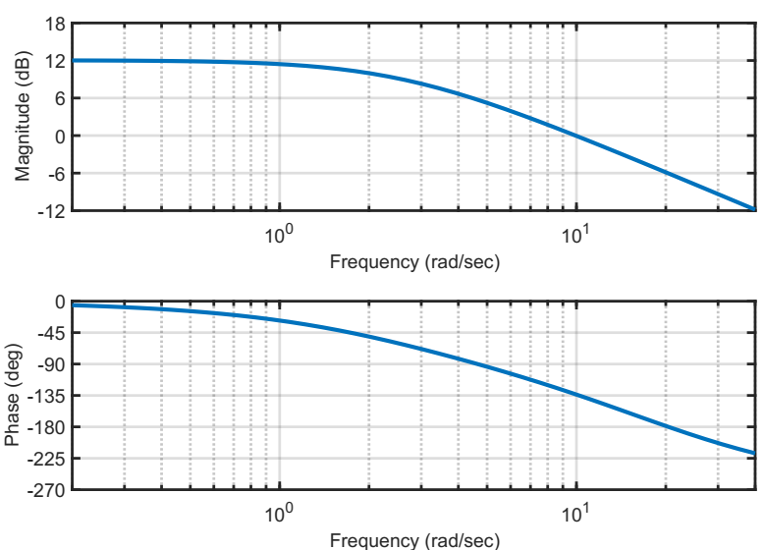
\includegraphics[width=0.9\textwidth]{figs/6.1.png}
\caption{Bode Plot}
\end{figure}
\begin{itemize}
    \item[(a)] What is the phase crossover frequency, $\omega_0$?
    \item[(b)] What is the gain margin, $g_0$, of the closed-loop? 
    \item[(c)] Is the closed-loop stable if the open-loop transfer function is $1.5L(s)$?
    \end{itemize}
\textbf{\textcolor{red}{Solution :}} \\
\begin{itemize}
    \item[(a)] $\omega_0 = 20 \text{rad}/\sec.$
    \item[(b)] $g_0 = 2$.
    \item[(c)] Yes. Because $1.5 < g_0 = 2$.
\end{itemize}

\clearpage
\subsection{Gain Crossover and Phase Margin Analysis}

Consider a standard closed-loop system with the loop transfer function $L(s)$ with the Bode plot below.  Assume the closed-loop is stable with the loop $L(s)$:
\begin{equation*}
    L(s) = \frac{-4s+72}{0.39s^2+8.02s+18}
\end{equation*}
\begin{figure}[h]
\centering
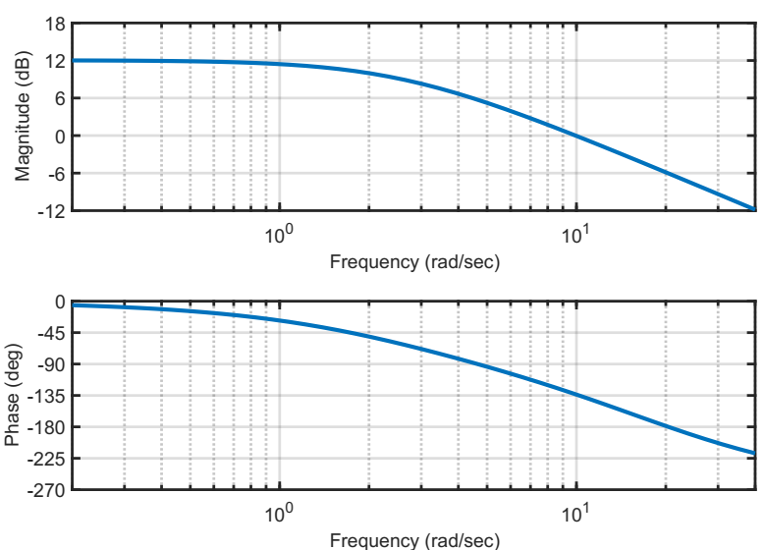
\includegraphics[width=0.9\textwidth]{figs/6.1.png}
\caption{Bode Plot}
\end{figure}
\begin{itemize}
    \item[(a)] What is the gain crossover frequency, $\omega_0$?
    \item[(b)] What is the phase margin, $\theta_0$, of the closed-loop? 
    \end{itemize}
\textbf{\textcolor{red}{Solution :}} \\
\begin{itemize}
    \item[(a)] $\omega_0 = 10\, \text{rad}/\sec.$
    \item[(b)] $\theta_0 = 45^{\circ}$.
\end{itemize}
\clearpage

\subsection{Bode Plot Analysis and Steady-State Response of a Linear System}

A linear system \(G(s)\) with input \(u\) and output \(y\) has the bode plot shown below:
\begin{itemize}
    \item[(a)] What is \(|G(10j)|\) in \(dB\) and actual units?
    \item[(b)] What is \(\angle G(10j)\) om degs and radians?
    \item[(c)] What is the output response \(y(t)\) in steady-state for the input \(u(t) = 2 \cos(10t)\)?
    \item[(d)] What is the steady-state value of \(y(t)\) if the input is a unit step \(u(t) = 1\) for all \(t \geq 0\)?
\end{itemize}
\begin{figure}[h]
\centering
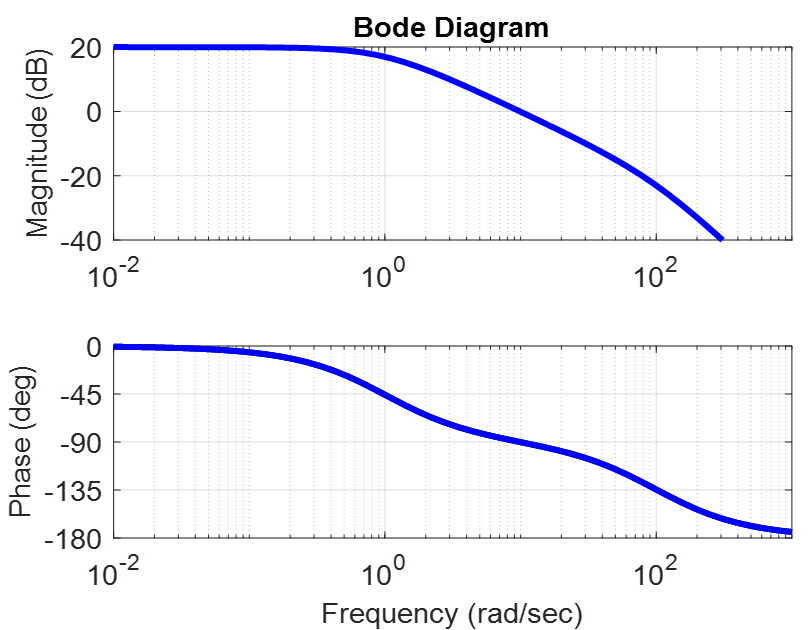
\includegraphics[width=0.6\linewidth]{figs/6.3ver2.png}
\caption{Bode Plot}
\end{figure}
\textbf{\textcolor{red}{Solution :}}
\begin{itemize}
    \item[(a)] \(|G(j10)| = 0 dB = 1\)
    \item[(b)] \(\angle G(j10) = -90 \text{deg} = -\frac{\pi}{2} \text{rad}\)
    \item[(c)] \(y(t) = 2|G(j10)|\cos(10t + \angle G(j10)) = 2 \cos(10t-\frac{\pi}{2}) \)
    \item[(d)] \(u(t) = \cos(\omega t) \quad \text{with} \quad \omega = 0\)
    \[|G(j0)| = 20 dB = 10 \quad \text{and} \quad \angle G(j0) = 0 \text{deg} = 0 \text{rad}\]
    Thus, we have:
    \[y(t) = |G(j0)| \cos(\omega t + \angle G(j0)) = 10 \]
\end{itemize}
\clearpage

\subsection{Closed-Loop Stability Analysis with Bode Plot}

Consider a standard closed-loop system with the loop transfer function $L(s)$ with Bode plot below.  Assume the closed-loop is stable with the loop $L(s)$.

\begin{equation}
    L(s) = \frac{-4s + 72}{0.39 s^2 + 8.02 s + 18}
\end{equation}

\begin{figure}[h]
    \centering
    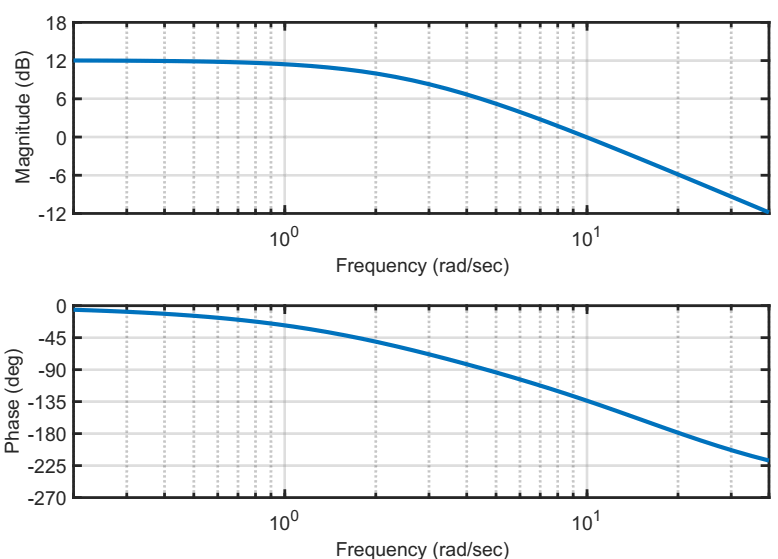
\includegraphics[width=\textwidth]{figs/6.4.png}
    \label{fig:bode-88}
    \caption{Bode Plot}
\end{figure}

\begin{itemize}
    \item[(a)] What is the gain cross-over frequency $\omega_0$ in rads/sec?
    \item[(b)] What is the phase margin, $\theta_0$, of the closed-loop in degrees?
    \item[(c)] What is the delay margin, $\tau_0$, of the closed-loop in seconds?
\end{itemize}

\textbf{\textcolor{red}{Solution :}}

\begin{itemize}
    \item [(a)] The gain cross-over frequency is $\omega_0 = 10$ rad/sec
    \item [(b)] The phase margin is $\theta_0 = 45 $ deg.
    \item [(c)] The delay margin is $\tau_0 = \pi/ 40 \approx 0.08$ secs.
\end{itemize}
\clearpage

\subsection{Deriving Transfer Function from Bode Plot for First-Order System}

The system \(G(s)\) is first-order. Determine the transfer function for this system from the Bode plot.
\begin{figure}[H]
    \centering
    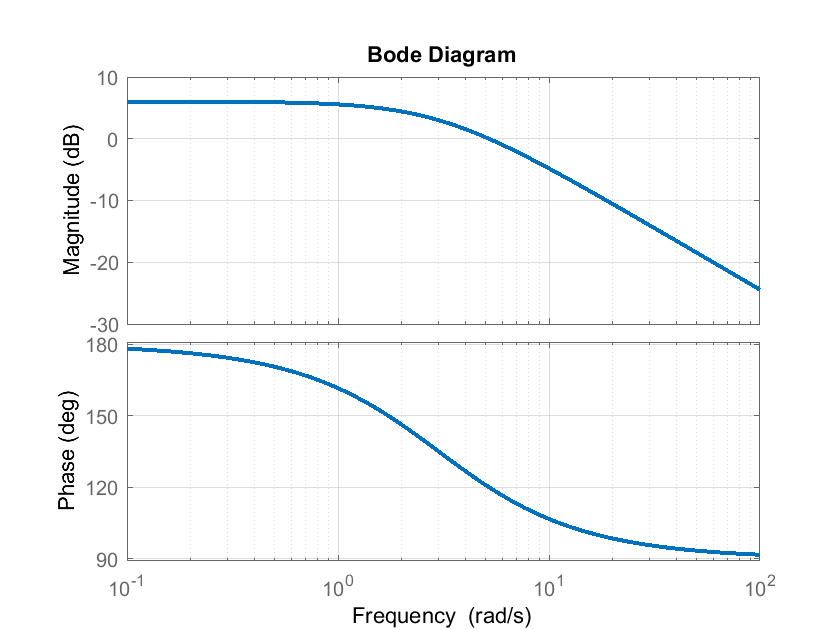
\includegraphics[width=0.7\textwidth]{figs/6.5.png}
    \caption{Bode Plot}
    \label{fig:89}
\end{figure}
\textbf{\textcolor{red}{Solution :}}
\[G(s) = - \frac{6}{s+3}\]
\clearpage

\subsection{Disk Margin}

Consider the following loop transfer function:
\begin{equation}
    L(s)  = \frac{4s+1}{s^3 + 4s - 2s + 0.5}
\end{equation}
Below is the Bode magnitude plot of the closed-loop sensitivity $S(s)$. 

\begin{figure}[h]
        \centering
        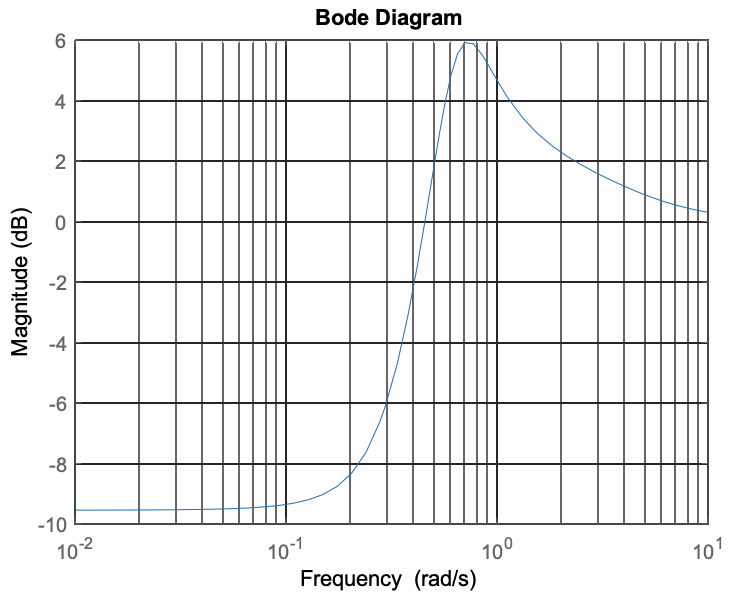
\includegraphics[width=0.7\textwidth]{figs/6.6.png}
        \label{fig:nyquist_92}
        \caption{Bode Plot}
\end{figure}

Compute the disk margin from the Bode magnitude plot of $S(s)$ 

\textbf{\textcolor{red}{Solution :}}

Since $d_{\text{min}} = \text{min}_{\omega} | 1 + L(j \omega) | $ and $S(j \omega) = \frac{1}{1 + L(j\omega)}$, the minimizing frequency will also maximize closed-loop sensitivity $\text{max}_\omega |S(j\omega)| = 6 dB \approx 2$ in absolute units. Therefore the disk margin is $d_{\text{min}} \approx  1/2$.
\clearpage

\subsection{Matching Transfer Functions with Their Corresponding Bode Plots}

Let \(G(s) = \frac{1}{s+1}\). Name each component \(K_i(s)\) below and match with the corresponding Bode plot for the loop \(L(s) = G(s) K_i(s)\).

\begin{enumerate*}
    \item[(i)] \(K_1(s) = 2\)
    \item[(ii)] \(K_2(s) = \frac{s+0.1}{s}\)
    \item[(iii)] \(K_3(s) = \frac{10}{s+10}\)
    \item[(iv)] \(K_4(s) = \frac{2s+10}{s+20}\)
\end{enumerate*}


\begin{figure}[H]
        \centering
        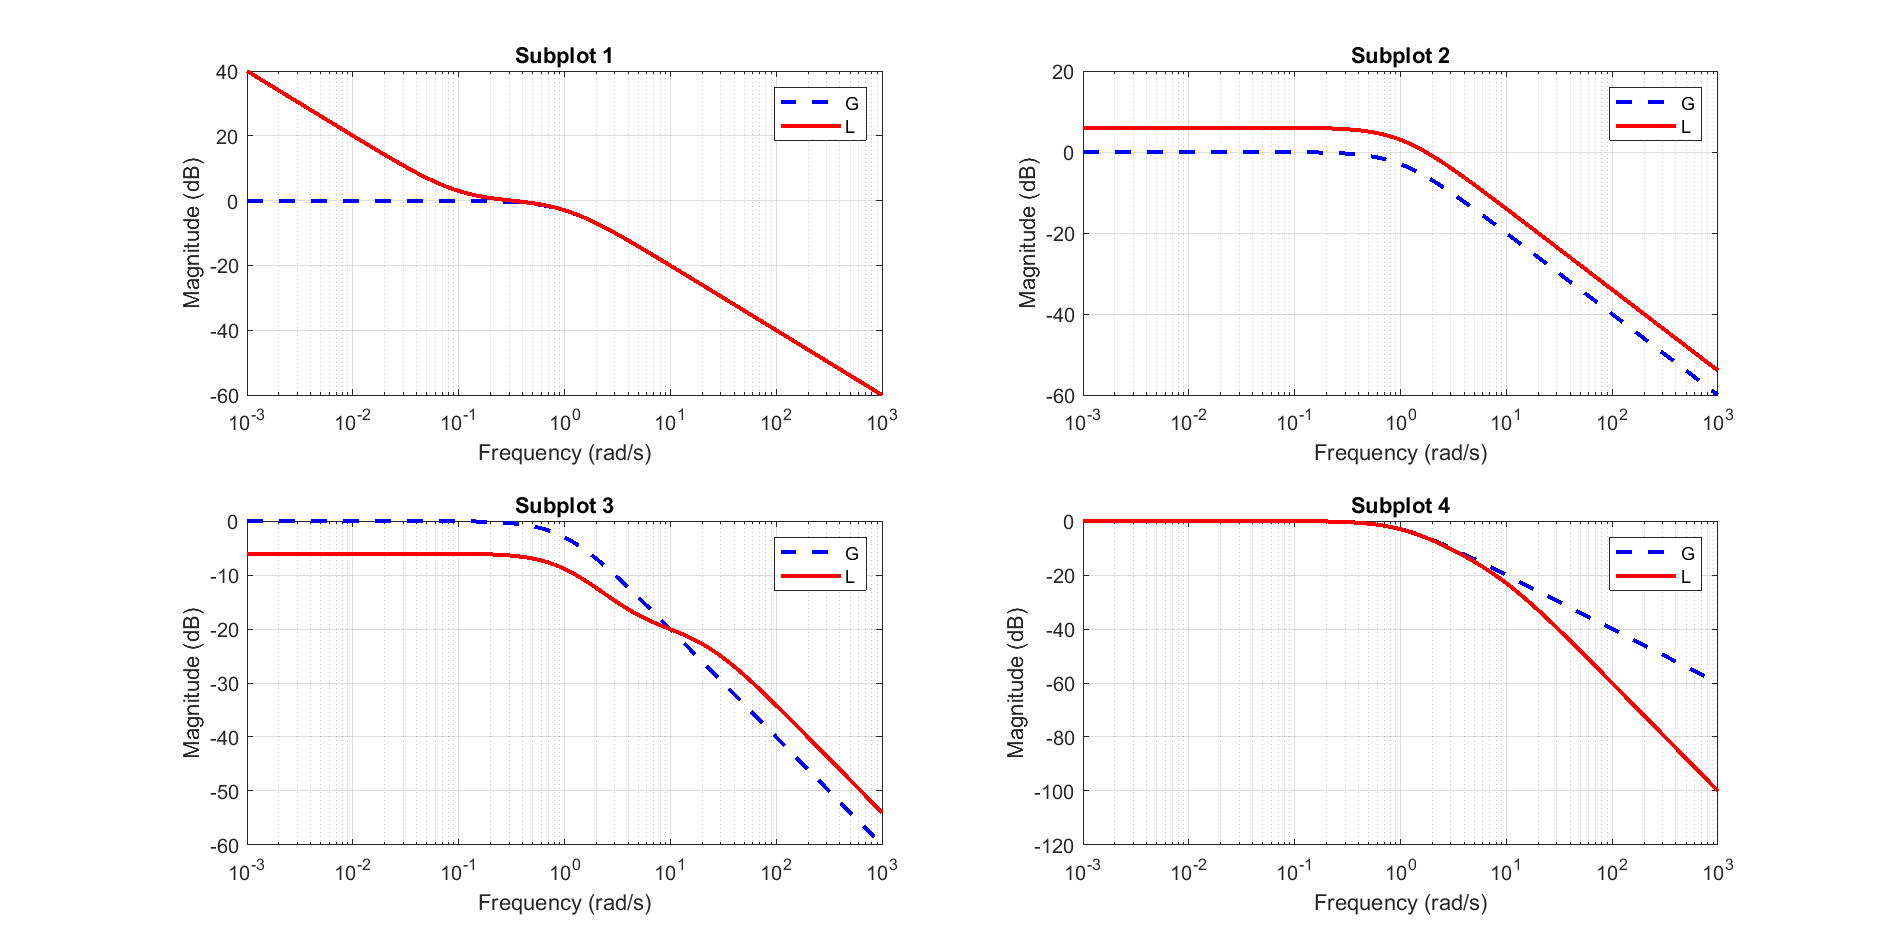
\includegraphics[width=\textwidth]{figs/6.7.png}
        \label{fig:nyquist_92}
        \caption{Bode Plots for Loop Transfer Functions \(L(s)\)}
\end{figure}
\textbf{\textcolor{red}{Solution :}}

\begin{enumerate*}
    \item[(i)] Subplot 2
    \item[(ii)] Subplot 1
    \item[(iii)] Subplot 4
    \item[(iv)] Subplot 3
\end{enumerate*}\\
\clearpage

\subsection{Design of a Proportional Controller Using Bode Plots}

Consider a feedback system where the plant $G(s)$ is stable and has the Bode magnitude plot shown below. We want to design a controller so that: i) the closed-loop is stable, ii) the system has a loop cross-over frequency near 50 rad/sec, and iii) the closed-loop can track $r(t) = \sin(0.1t)$ with less than 1\% error.
\begin{figure}[h]
    \centering
    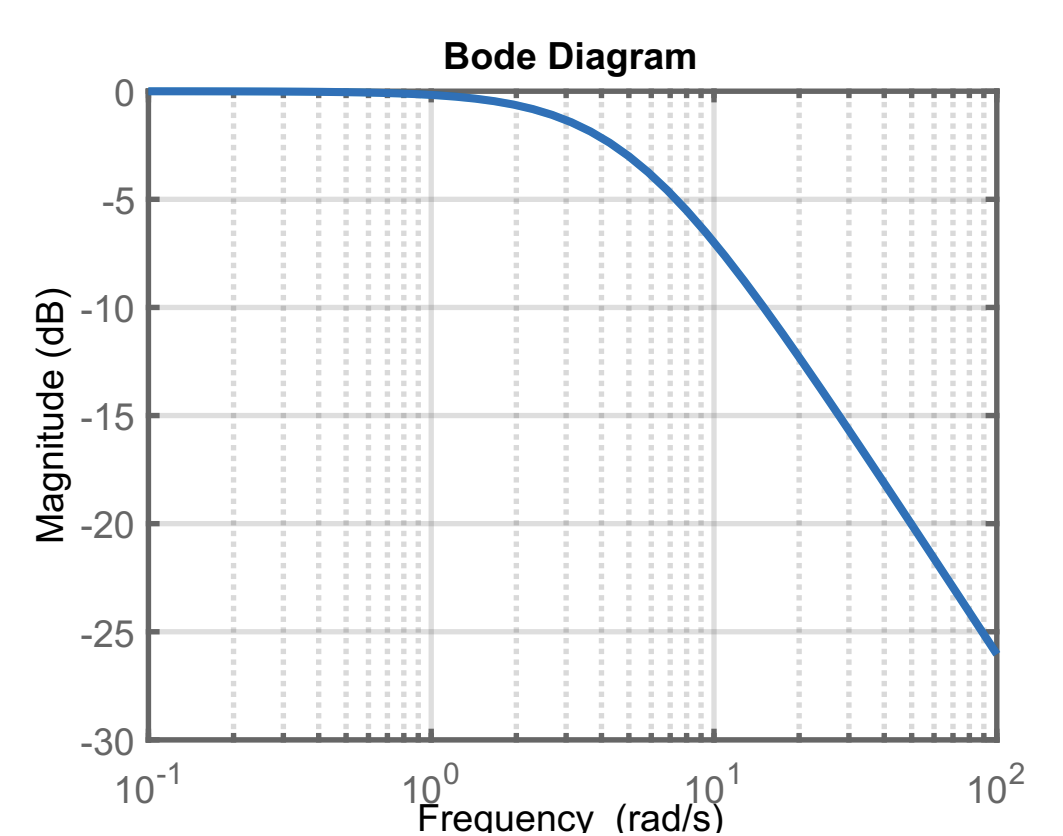
\includegraphics[width=0.7\textwidth]{figs/6.8.png}
    \caption{Bode Plot}
    \label{fig:bode_94}
\end{figure}

\begin{itemize}
    \item[(a)] Using the Bode diagram, choose a gain $K_p$ so that $K_p G(s)$ has the desired cross-over frequency of $50$ rad/sec.
    \item[(b)] Convert the requirement (iii) into a requirement on the closed-loop transfer function $L(s) = G(s) K(s)$.
\end{itemize}

\textbf{\textcolor{red}{Solution :}}

\begin{itemize}
    \item[(a)] $|K_p G(j 50)| = 1$ implies that $K_p = 1/ |G(j 50)| \approx 1/ 0.1 = 10$
    \item[(b)] With $r(t)=\sin(0.1 t)$, and $S(j w) = \frac{1}{1+L(j \omega)}$ the response from $r \rightarrow e$, then we must have $|S(j \omega) |\sin(0.1 t + \measuredangle S(j \omega)) \leq 0.01$. Therefore $|S(j \omega)| = |\frac{1}{1 + L(j \omega)}| \leq 0.01$ and so $100\leq |1+L(j\omega)| \approx | L(j\omega)|$. 
\end{itemize}
\clearpage

\subsection{Design of a Proportional Controller Using Bode Plots}

Consider a feedback system where the plant $G(s)$ is stable and has the Bode magnitude plot shown below. We want to design a controller so that: i) the closed-loop is stable, ii) the system has a loop cross-over frequency near $1$ rad/sec, and iii) the gain from the noise $n$ to the output $y$ is $\leq 0.001$ for $\omega \geq 100$ rad/sec. 

\begin{figure}[H]
    \centering
    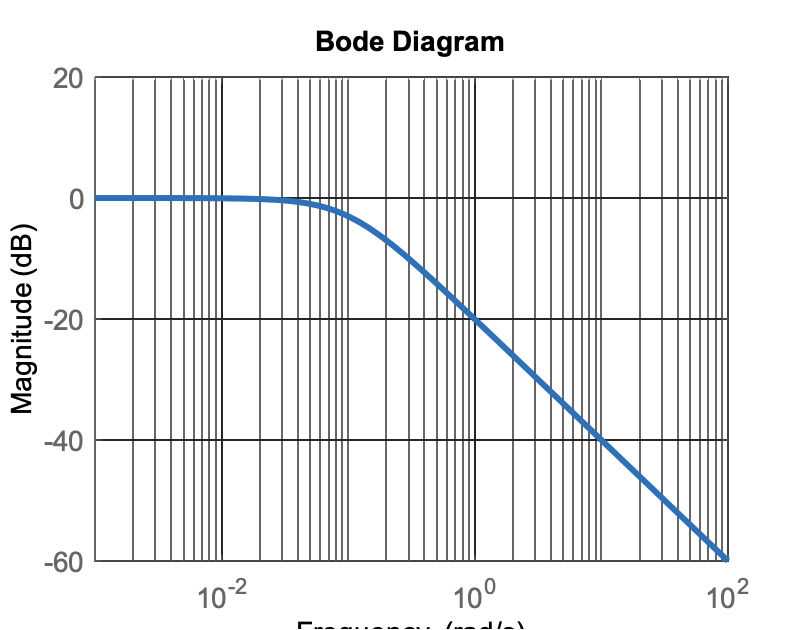
\includegraphics[width=0.7\textwidth]{figs/6.9.png}
    \label{fig:bode_94}
    \caption{Bode Plot}
\end{figure}

\begin{itemize}
    \item[(a)] Using the Bode diagram, choose a gain $K_p$ so that $K_p G(s)$ has the desired cross-over frequency of $1$ rad/sec.
    \item[(b)] Convert the requirement (iii) into a requirement on the closed-loop transfer function $L(s) = G(s) K(s)$. The transfer function from noise \(n\) to \(y\) is $T_{n \rightarrow y} = -\frac{L(j \omega)}{1+L(j \omega)}$
\end{itemize}

\textbf{\textcolor{red}{Solution :}}

\begin{itemize}
    \item[(a)] $|K_p G(j 1)| = 1$ implies that $K_p = 1/ |G(j 1)| \approx 1/ 0.1 = 10$.
    \item[(b)] With $n(t)=\sin(\omega t)$, and $-T(j w) = -\frac{L(j \omega)}{1+L(j \omega)}$ the response from $n \rightarrow y$, then we must have $-|T(j \omega) |\sin(\omega t + \measuredangle T(j \omega)) \leq 0.001$ for all $\omega \geq 100$. Therefore we should have $|T(j \omega)| = |\frac{L(j\omega)}{1+L(j\omega)}| \leq 0.001$ for all $\omega \geq 100$. 
\end{itemize}

\clearpage
\subsection{Estimating Steady-State Output from Bode Plot Analysis}

The Bode plot for the system with transfer function
\begin{equation}
    \frac{X(s)}{G(s)} = \frac{s^2+0.002s+10000}{(s+0.01)(s+1000)}
\end{equation}
is shown in the figure below. Estimate the steady-state output \(x_{ss}(t)\) corresponding to the input \(f(t) = 0.0001\sin 0.0001t + \sin 100t + \sin 10000t\).
\begin{figure}[H]
    \centering
    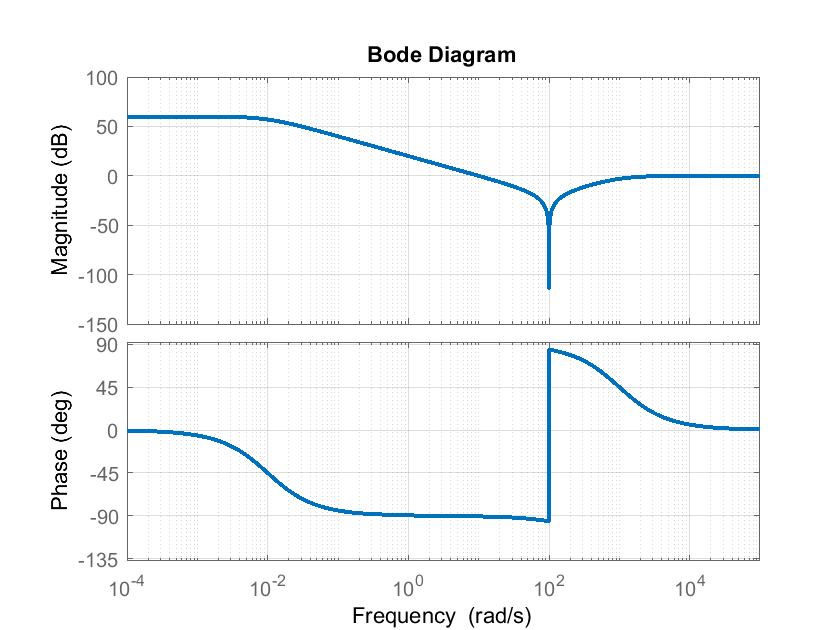
\includegraphics[width=0.8\textwidth]{figs/6.10.png}
    \label{fig:99}
    \caption{Bode Plot}
\end{figure}
\textbf{\textcolor{red}{Solution :}} \\
We gave three periodic terms, so we consult the Bode plot at each frequency to determine the gain and the phase shift of each.
\begin{itemize}
    \item The frequency \(\omega = 10^{-4}\) is not included in the Bode plot, but the plot is level at \(10^{-3}\) so we assume the same gain of approximately \(60 dB\). Likewise, the phase shift is not shown, but appears to be very close to zero. Since \(60 dB = 20log(|G|) \rightarrow |G| = 10^3\), we have an output component of \(0.1 \sin(10^{-4}t)\)/
    \item At \(\omega = 10^2\), the gain is \(<-150 dB\). This gain effectiverly attenuates this signal to zero.
    \item At \(\omega = 10^4\), the gain is approximately \(0 dB\), which is a gain of \(1\). The phase shift is also effectively \(0\), so this gives a component of \(\sin(10^4t)\).
\end{itemize}
Therefore, our output is approximately: \(x(t) = 0.1 \sin(10^{-4}t) + \sin(10^4t)\).
\clearpage

\subsection{Matching Step Responses with Their Corresponding Bode Plots}

Match the Bode plots 
\begin{figure}[H]
    \centering
    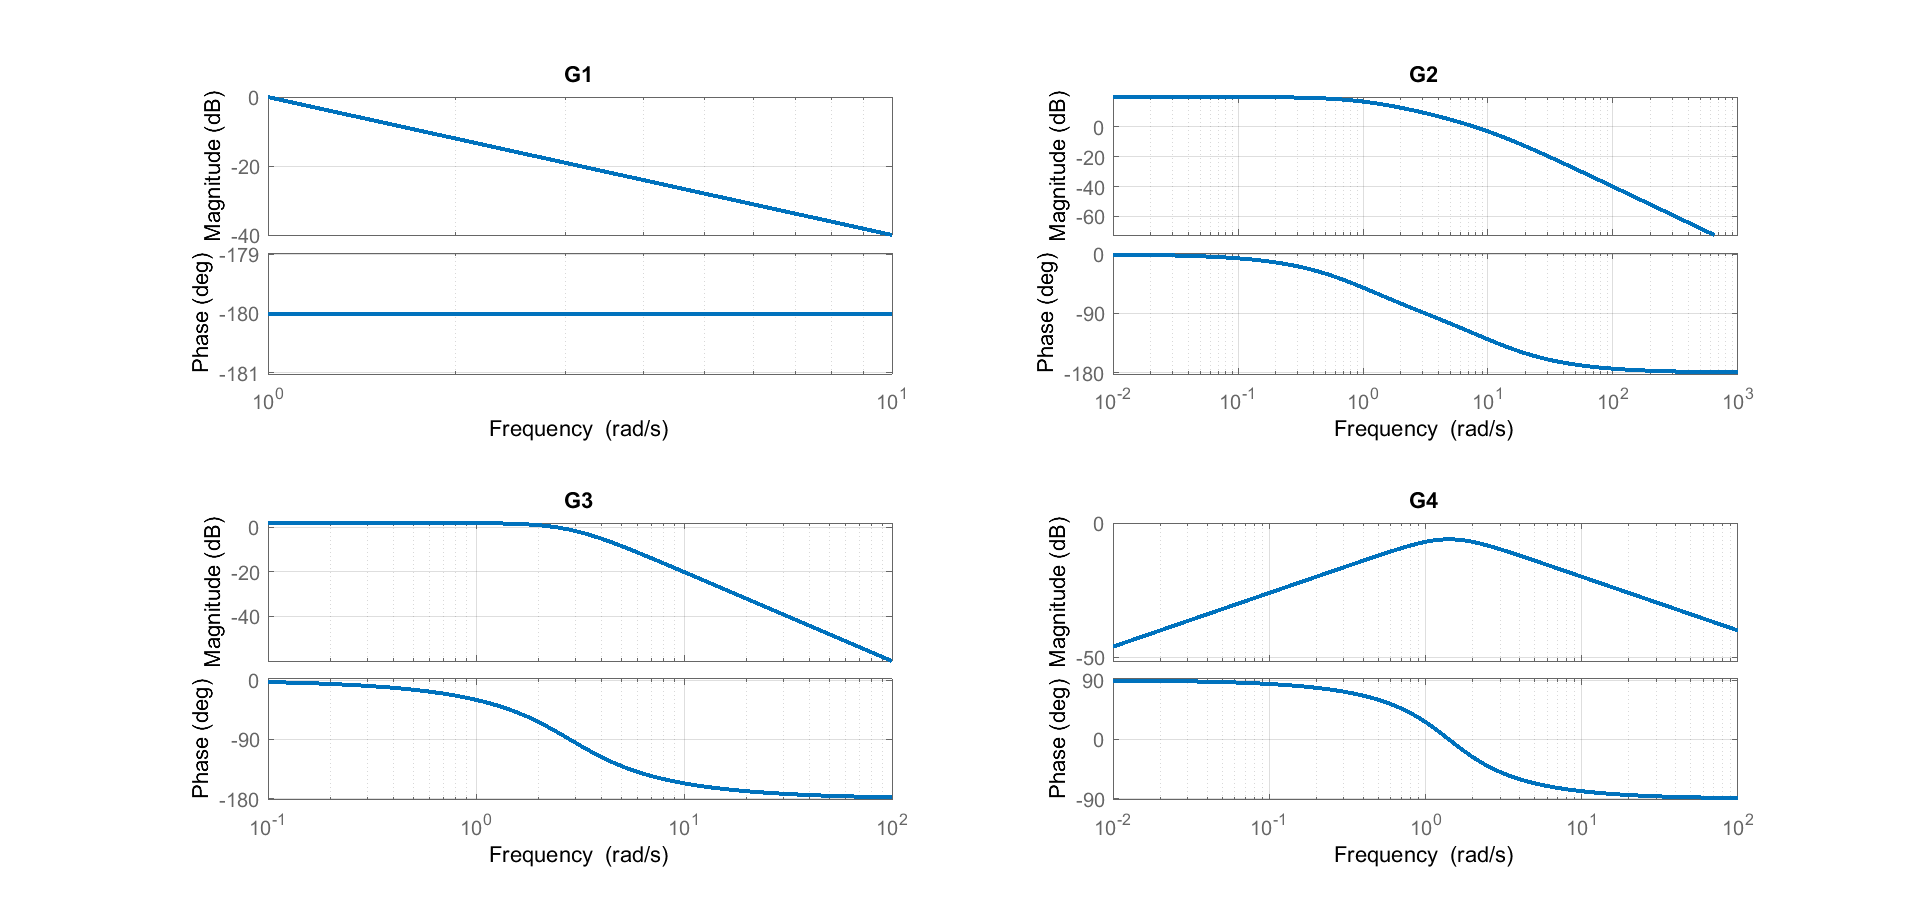
\includegraphics[width=\textwidth]{figs/6.11-1.png}
    \label{fig:99}
    \caption{Bode Plots}
\end{figure}
with the step responses.
\begin{figure}[H]
    \centering
    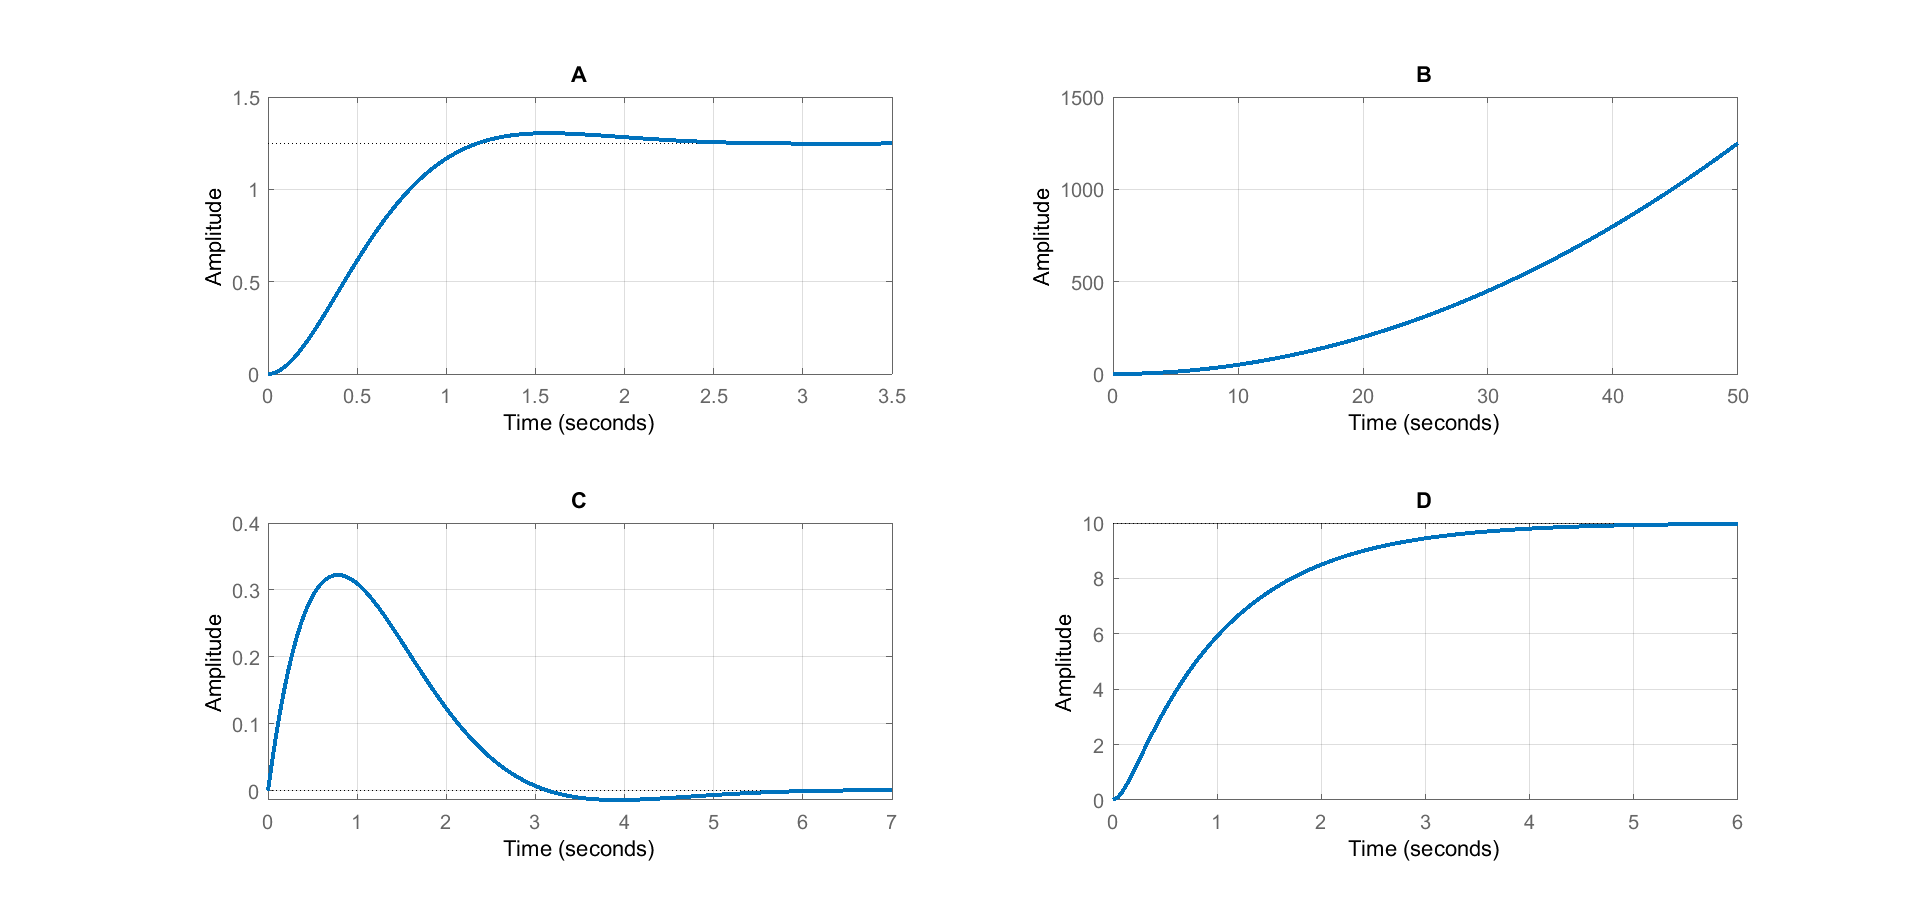
\includegraphics[width=\textwidth]{figs/6.11-2.png}
    \label{fig:99}
    \caption{Step Responses}
\end{figure}
\textbf{\textcolor{red}{Solution :}} \\
\(G_1-B,G_2-D,G_3-A,G_4-C\)
\clearpage

\subsection{Lag Controller Design}


Design a lag controller that provides PM of at least \(60^{\circ}\) and steady-state tracking of constant references within \(10 \%\) for the following system
\[
G(s)=\frac{10}{\left(\frac{s}{0.2}+1\right)\left(\frac{s}{0.5}+1\right)}
\]
Compute the PM and steady-state tracking error for the following controller to verify that the specs are met:
    \[
        K D(s)=0.4 \frac{s+0.05}{s+0.02}
    \]


\textbf{\textcolor{red}{Solution :}} \\


In Fig. \ref{fig:prb23}(a), we can see that \(\mathrm{PM}=61.7 \mathrm{deg}, \omega_{c}=0.52\), and \(\mathrm{GM}=\infty\) for the system with controller $ K D(s)=0.4 \frac{s+0.05}{s+0.02}$. For steady-state error for constant input:
\[
e(\infty)=\left.\frac{1}{1+K D(s) G(s)}\right|_{s=0}=\frac{1}{1+0.4 \times 2.5 \times 10}=\frac{1}{11}<0.1
\]
\begin{figure}[h!]
    \centering
    \begin{subfigure}[b]{0.45\textwidth}
    \centering
    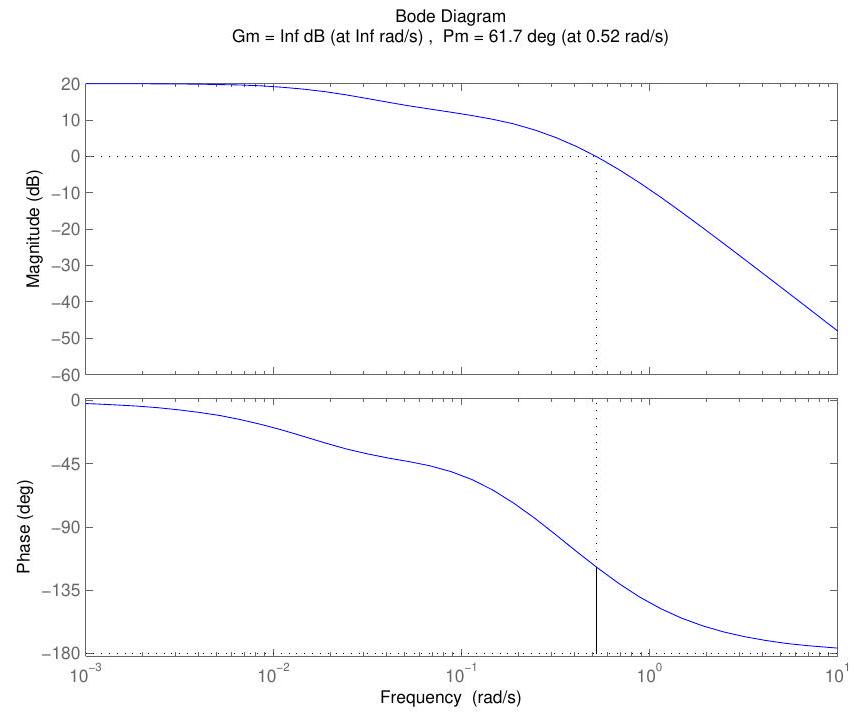
\includegraphics[width=\textwidth]{figs/6.12-1.jpg}
     \caption{Bode plot using given controller}
     \end{subfigure}
     \begin{subfigure}[b]{0.45\textwidth}
     \centering
        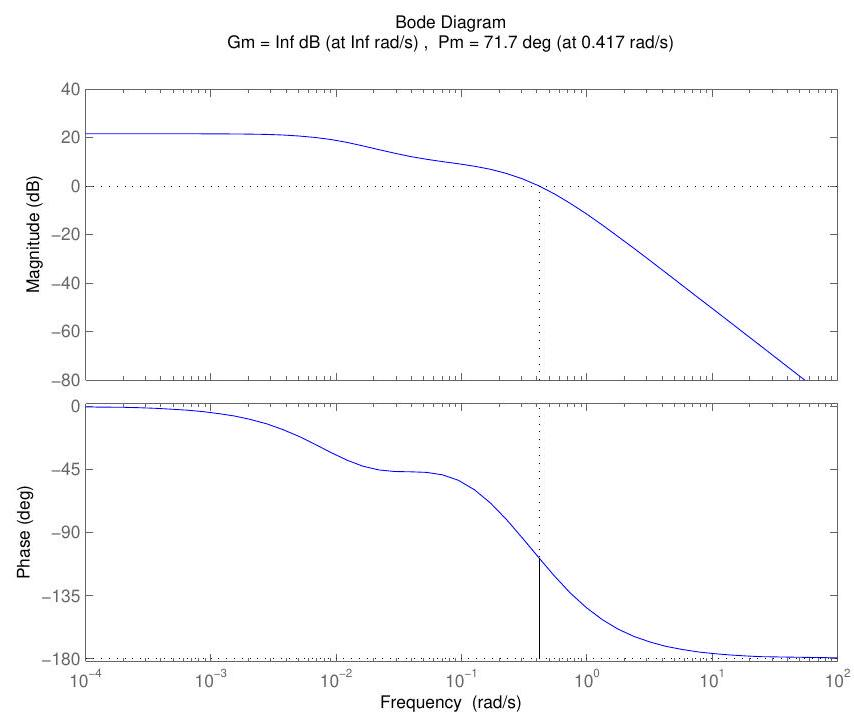
\includegraphics[width=\textwidth]{figs/6.12-2.jpg}
        \caption{Bode plot using modified controller}
     \end{subfigure}
     \caption{Bode plots} \label{fig:prb23}
\end{figure}
\clearpage

\subsection{Closed-Loop Poles}  
Consider the transfer function 
\[
G(s)=\frac{1}{(s - 1)(s^2 + 2s + 5)}
\]
Assume standard feedback configuration with K as the controller. Using the Bode plots of KG(s) explain how you can confirm the
presence of $j\omega$-axis closed-loop poles if $K=5$ or $K=8$. You can use the following bode plot to answer the question. \\

\begin{figure}[H]
    \centering
    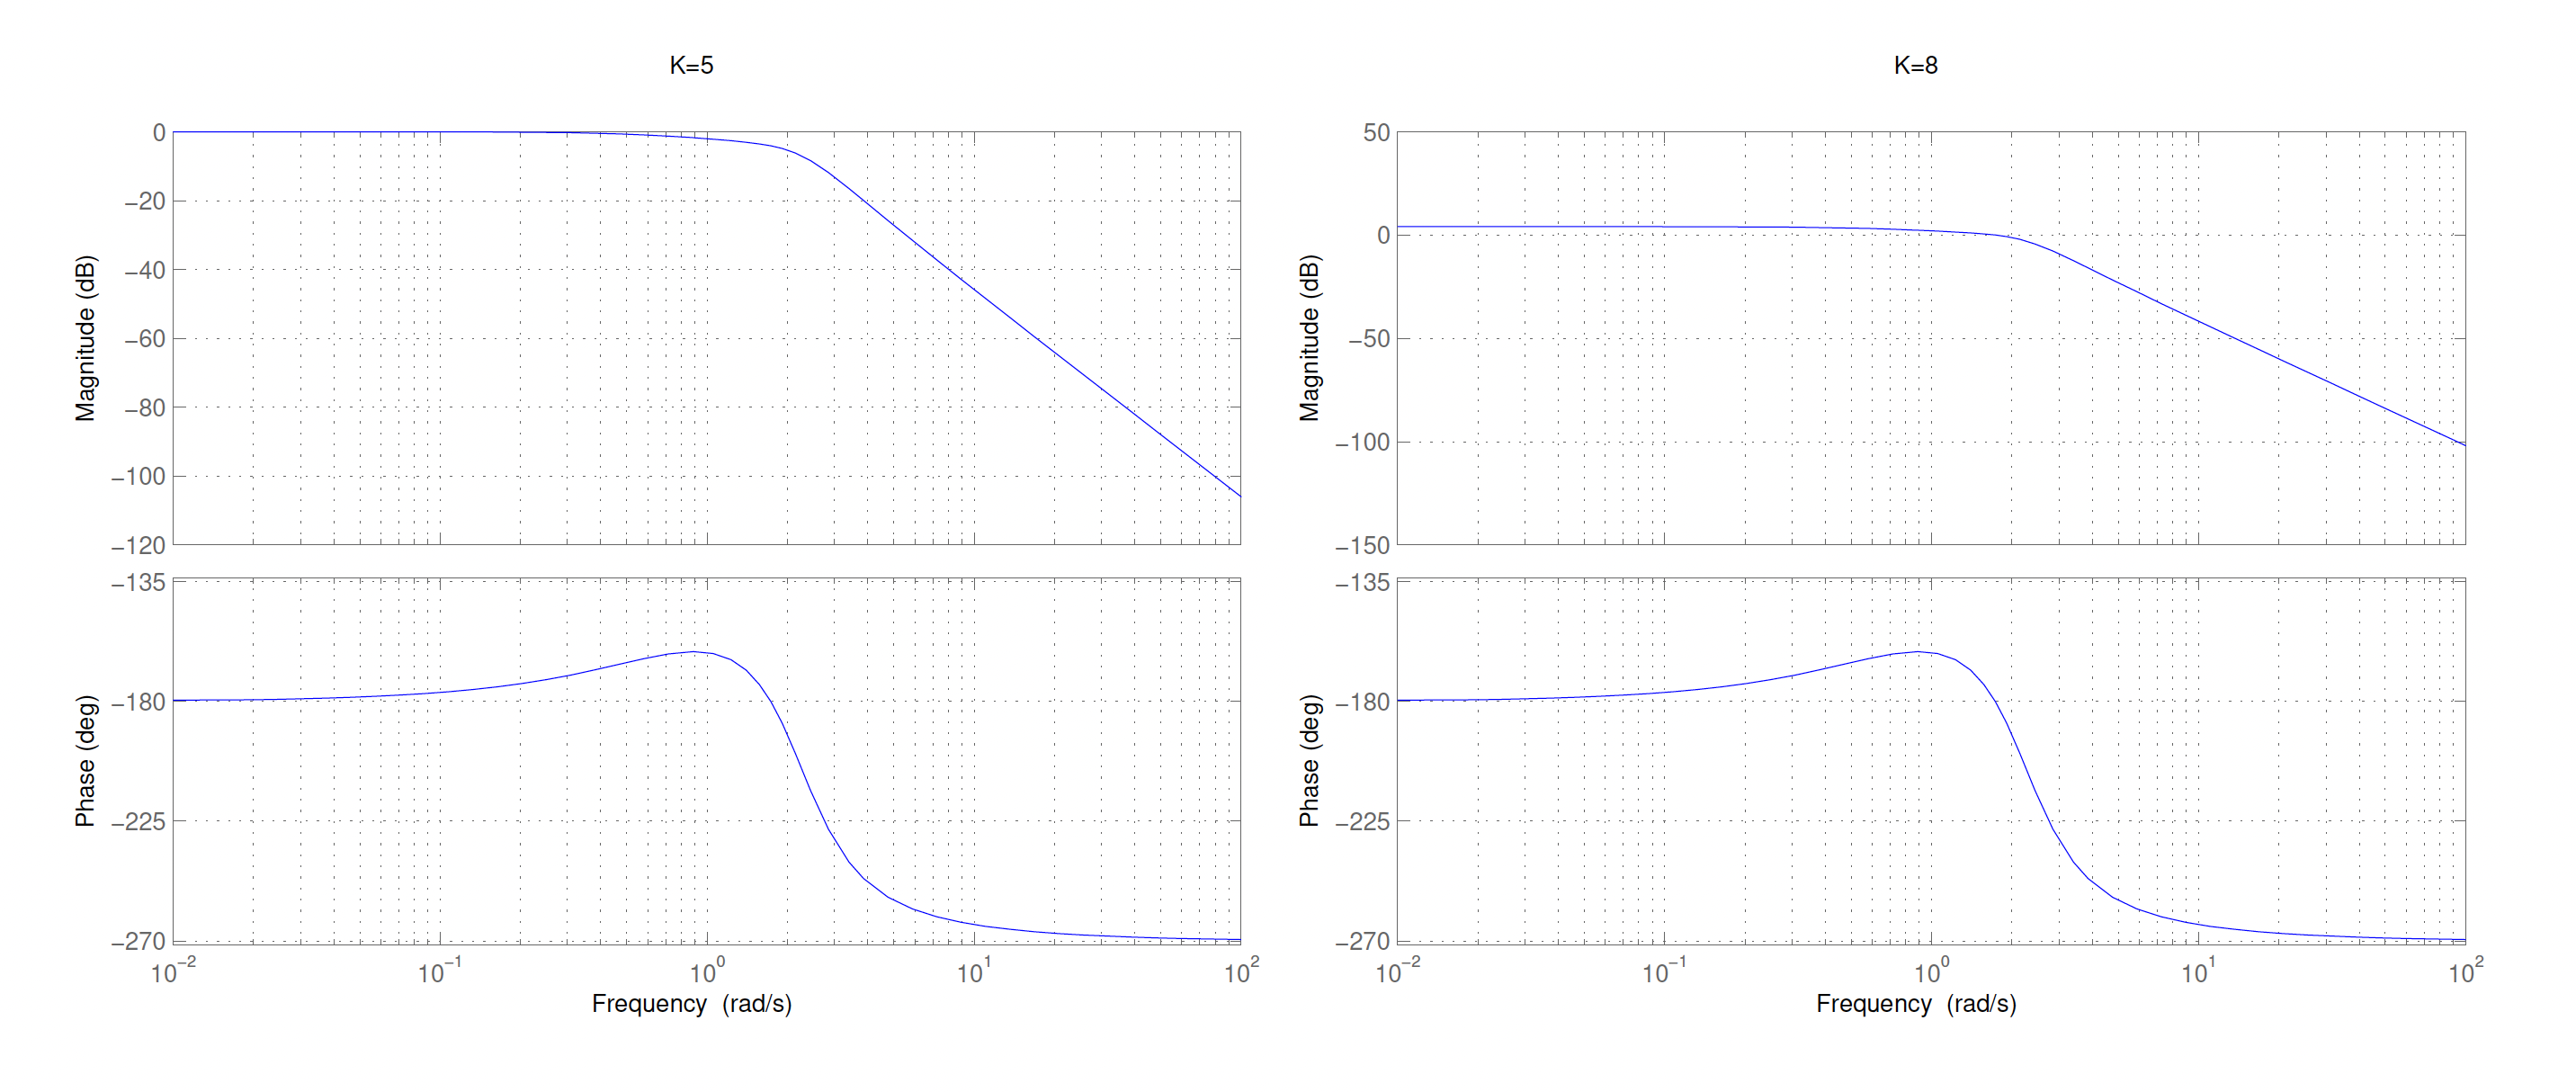
\includegraphics[width=1\linewidth]{figs/6.14.png}
    \caption{Bode Plots}
    \label{fig:prb30}
\end{figure}


\textbf{\textcolor{red}{Solution :}} \\
According to the bode plots given below for K = 5 and K = 8, we can see that both GM and PM are zero which confirm the presence of $j\omega$-axis closed-loop poles.
\clearpage

\subsection{Phase Margin}

Consider the transfer function 
\[
G(s)=\frac{1}{(s - 1)(s^2 + 2s + 5)}
\]
Assume standard feedback configuration with K as the controller. What is the largest possible phase margin that can be achieved for this system? Determine the gain K for which it is achieved. You can use the following bode plot to answer the question.\\

\begin{figure}[H]
    \centering
    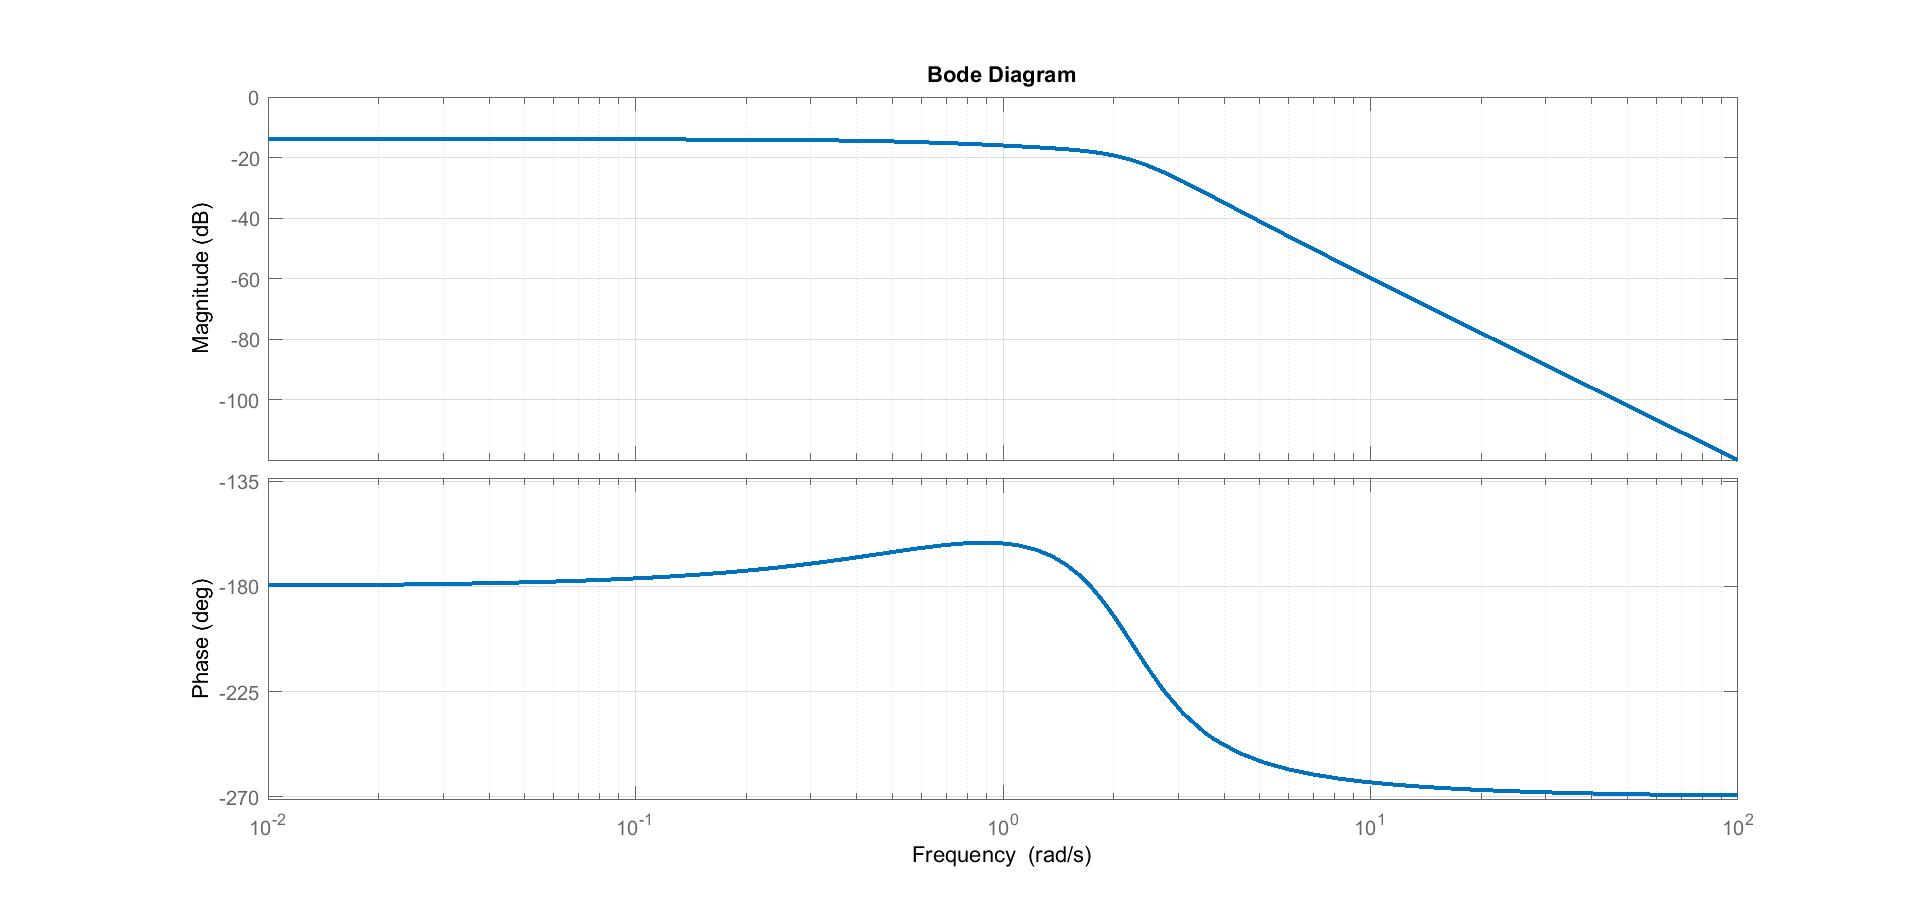
\includegraphics[width=1\linewidth]{figs/6.15.jpg}
    \caption{Bode Plot}
    \label{fig:prb31}
\end{figure}

\textbf{\textcolor{red}{Solution :}} \\
According to Bode plot given below, the maximum phase (and PM in this case) achieved on $\omega\approx 1$ (rad/sec), so we need to choose K in such a way that this is also equal to $\omega_c$. The result would be therefore be $K \approx 6.3$.
\clearpage

\subsection{Phase Margin}
Consider the system 
\[
G(s)=\frac{1}{(s - 1)(s+1)}
\]
\begin{itemize}
    \item [(a)] Design a PD controller that achieves phase margin $PM \approx 90^\circ$ and closed-loop bandwidth $\omega_{BW} \approx 10$. Verify that the specs are met.
    \item[(b)] Can you modify the above design to get $\omega_{BW} \approx 1$, while maintaining $PM \approx 90^\circ$? Explain how or why not.
\end{itemize}

\textbf{\textcolor{red}{Solution :}} \\
\begin{itemize}
    \item [(a)] The bode plot of G(s) given below shows that we have a phase margin of  $PM \approx 52^\circ$ (but small $\omega_c$). We want our PD controller to increase $\omega_c$ as well as PM.

    $D(s) = K(\tau s + 1)$, we choose $\frac{1}{\tau}  \ll 10$ to make sure the gain is high enough at $\omega_c = 10$. Also, we choose $\frac{1}{\tau} < 1$ to make sure that magnitude slope at $\omega_c = 10$ is -1.

    Let $\tau=2$ and $K\left| \frac{2 j \omega_c +1}{j \omega_c (j \omega_c+1)}\right|_{\omega_c = 10} =1 \implies  K \approx 5 \implies D(s) = 5(2 s + 1)$

    \begin{figure}[h!]
    \centering
    \begin{subfigure}[b]{0.5\textwidth}
    \centering
    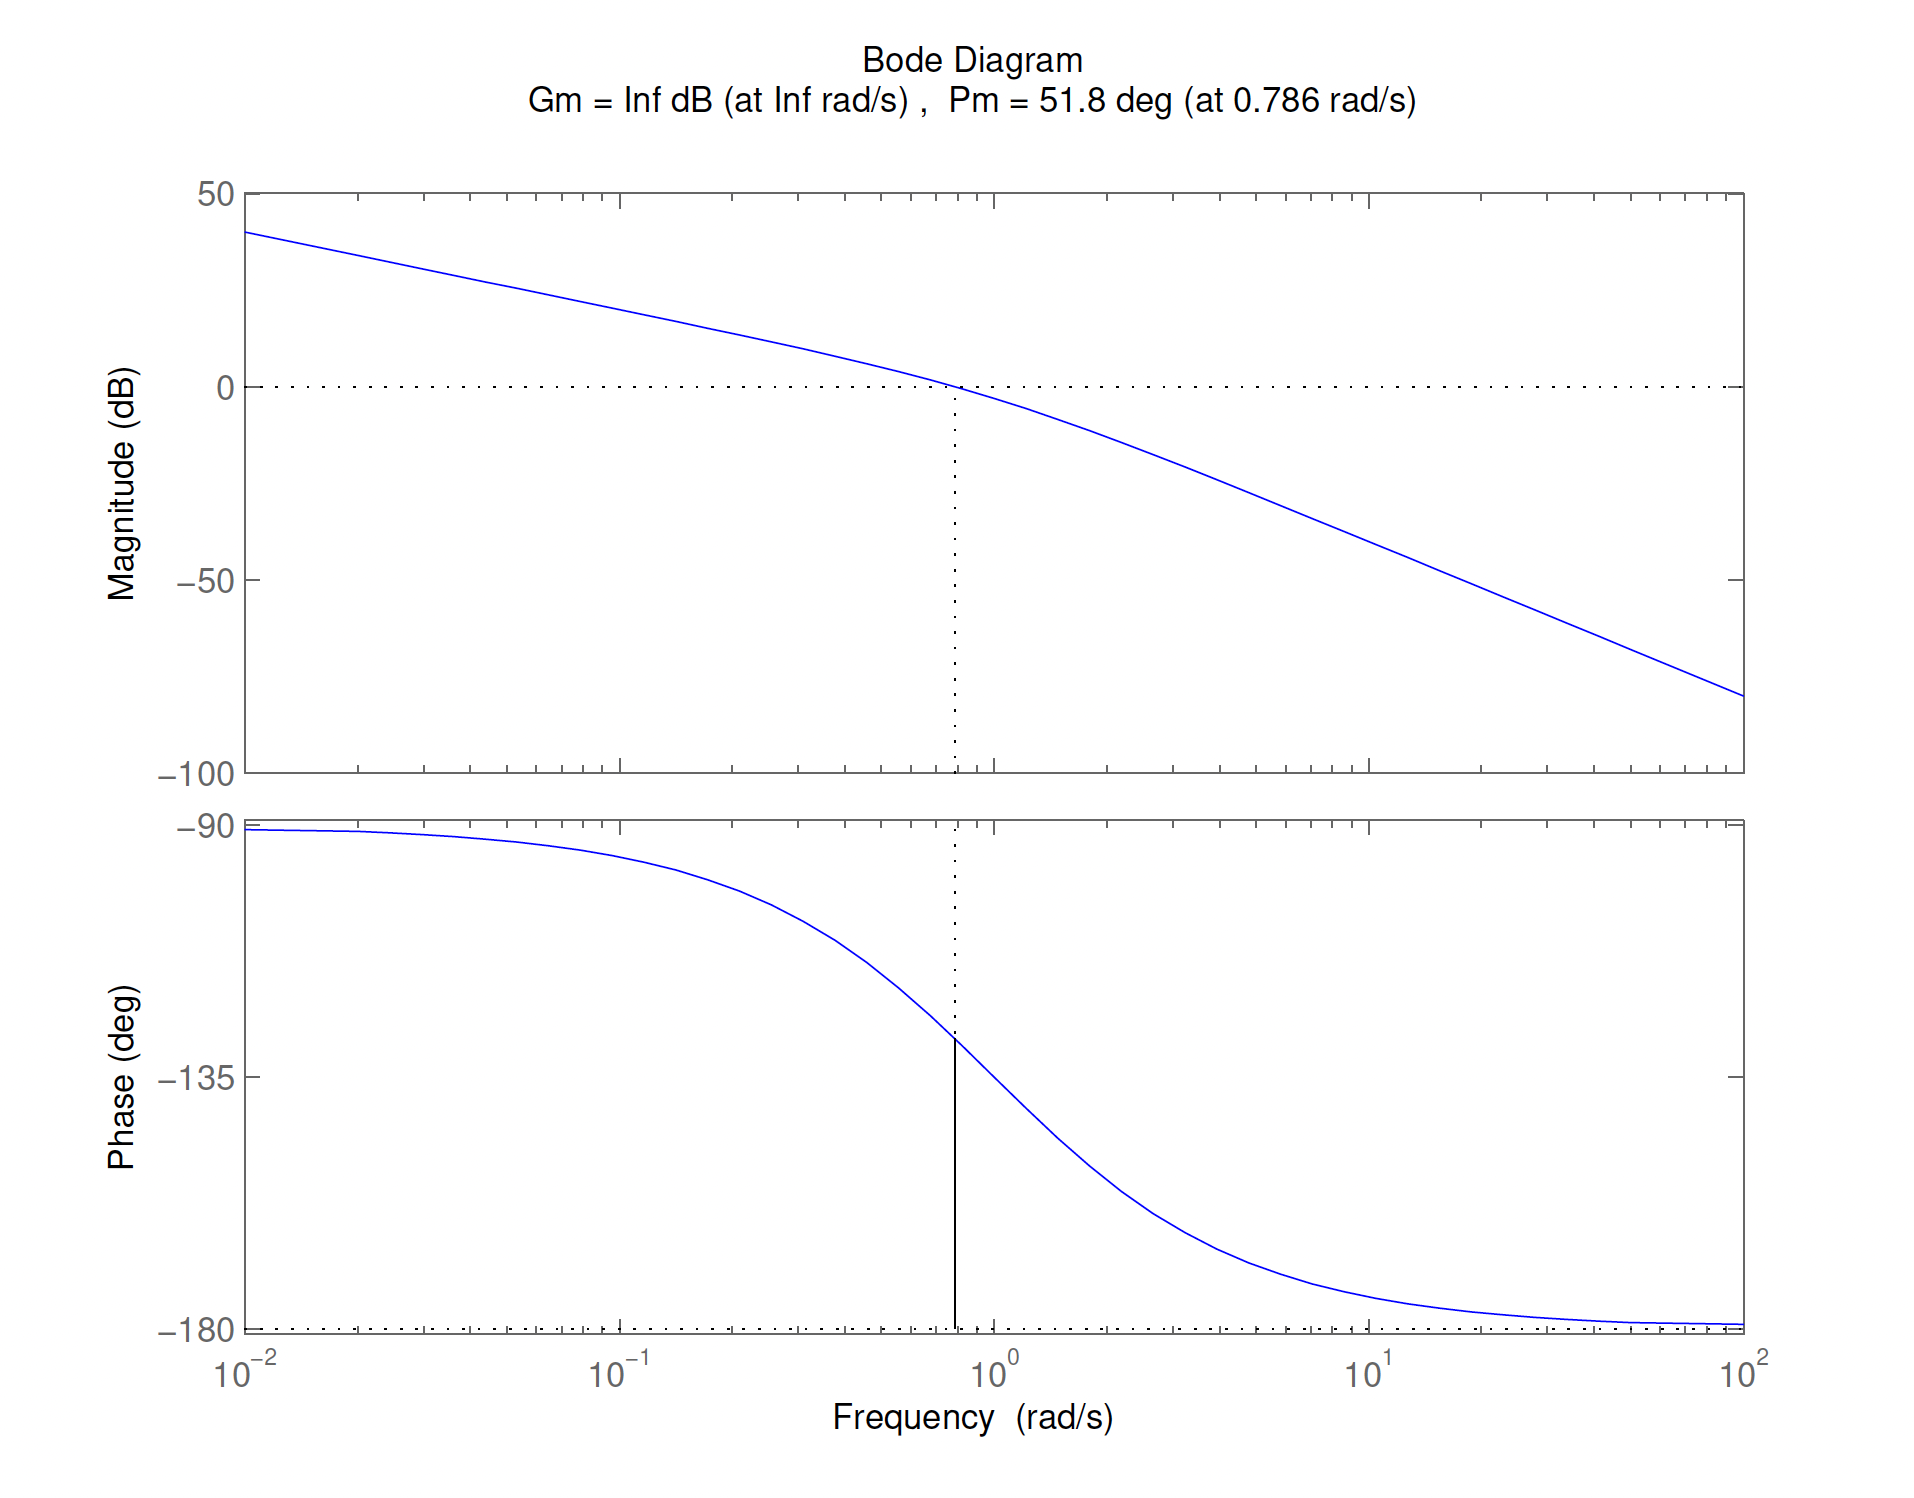
\includegraphics[width=\textwidth]{figs/6.16-1.png}
     \caption{Bode Plot of the System}
     \end{subfigure}
     \begin{subfigure}[b]{0.47\textwidth}
     \centering
        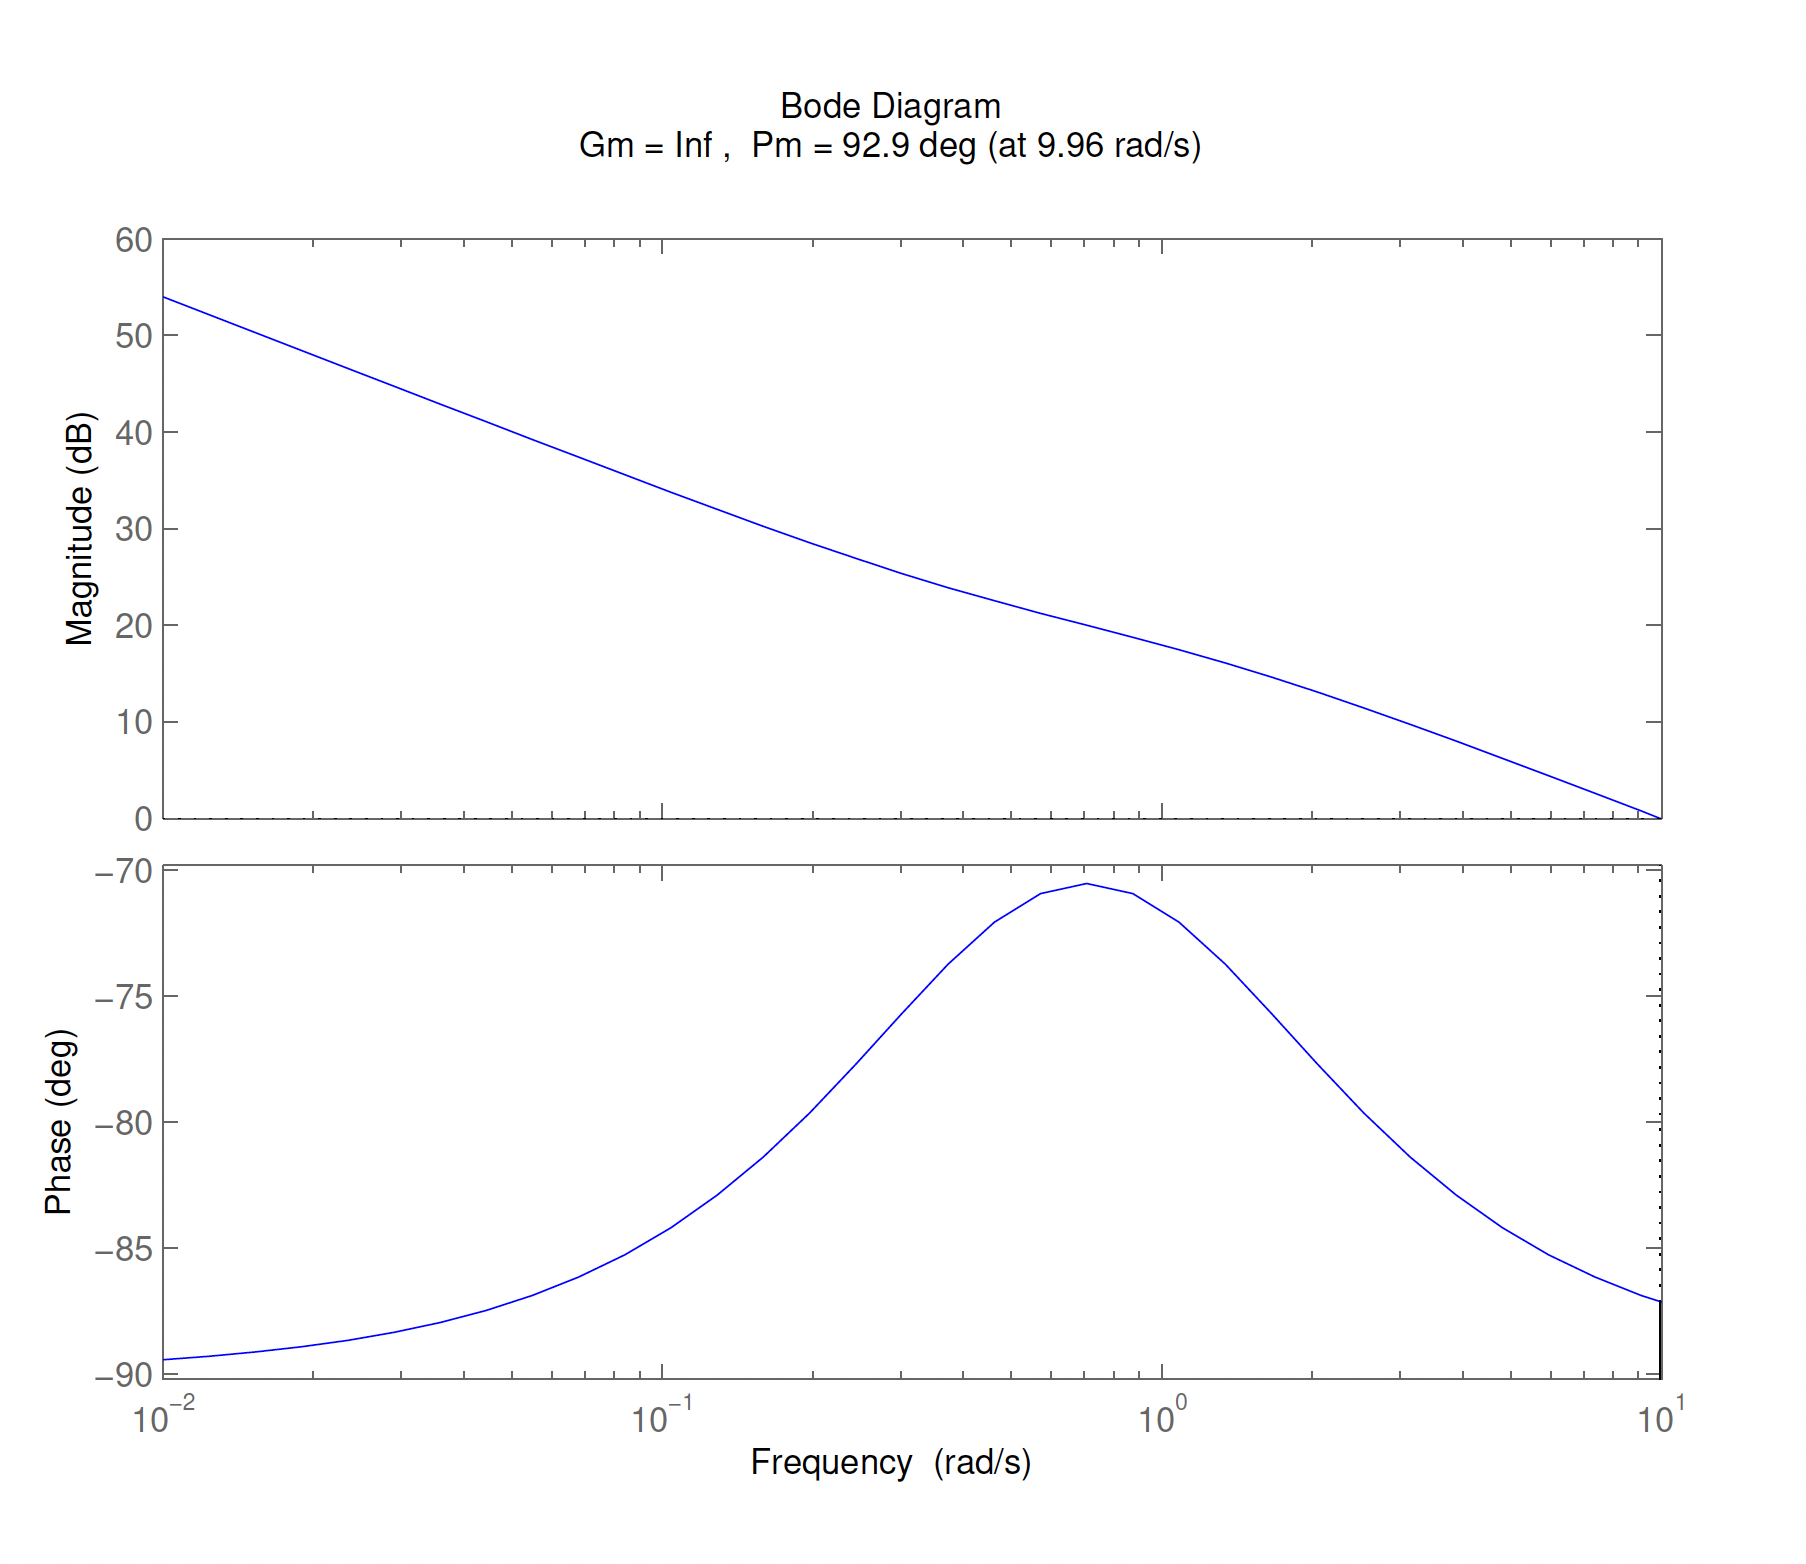
\includegraphics[width=\textwidth]{figs/6.16-2.png}
        \caption{Bode Plot of the Closed Loop System}
     \end{subfigure}
     \caption{Bode Plots} \label{fig:prb24}
\end{figure}


    \item[(b)] Achieving $\omega_{BW} = 1$ and $PM \approx 90^\circ$ is impossible unless we cancel the pole at $s = -1$ i.e.  $D(s) = s + 1$ . Because there is a break point at $\omega=1$ so we can't maintain slope = -1 on that point. Therefore, we cannot make $\omega_{BW} = 1$ and $PM \approx 90^\circ$ unless we take D(s) = s + 1. 
\end{itemize}
\clearpage

\section{Root-Locus Design}
\subsection{Root Locus Sketches of Transfer Functions}

Sketch the root loci for the following $L(s)$ by hand. Recall that the root locus plots how the solutions of $1+K L(s)=0$ vary as $K$ goes from 0 to $+\infty$.
\begin{align*}
    (a) \quad L(s)&=\frac{1}{s^2+2 s+20} \quad \qquad (b) \quad L(s)=\frac{s-3}{s^2+2 s+20} \\
    (c) \quad L(s)&=\frac{(s+1)(s+2)}{s\left(s^2+4\right)\left(s^2+5\right)}  \quad (d) \quad L(s)=\frac{s+3}{s^5+1}
\end{align*}

\begin{figure}[H]
    \centering
    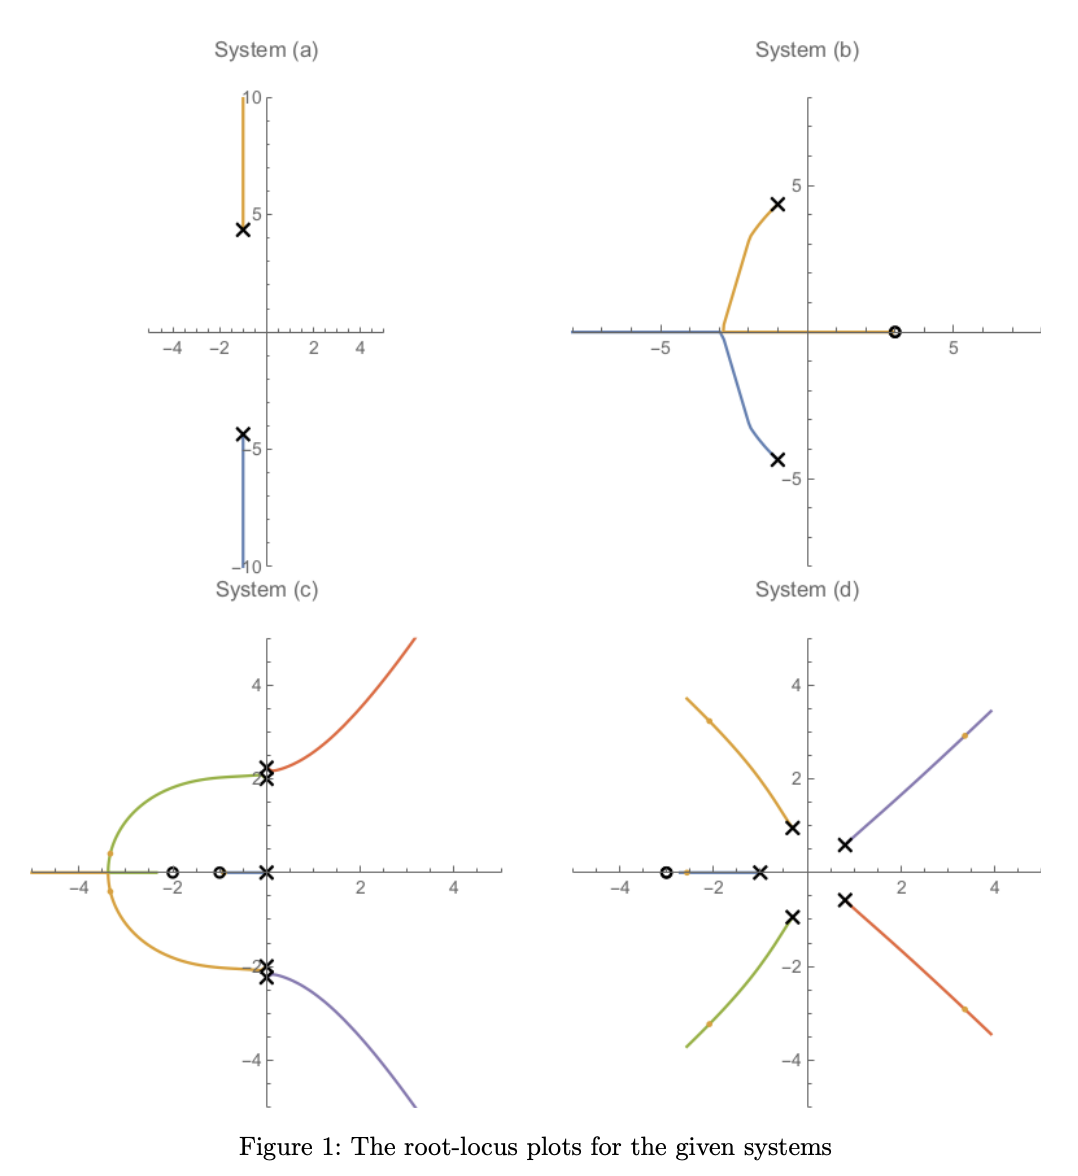
\includegraphics[width=0.55\linewidth]{figs/7.1.png}
    \caption{Root Locus for Systems}
    \label{fig:prb3}
\end{figure}

\textbf{\textcolor{red}{Solution :}} \\
The application of Rules for the given systems results in the following table: \\
\begin{table}[H]
    \centering
    \begin{tabular}{|c|c|c|c|c|}
    \hline
       Rule / System System   &  System (a) & System (b) & System (c) & System (d) \\
       \hline
        No. of branches & 2 & 2& 5 & 5 \\
       \hline
        Branch starts & $-1 \pm \sqrt{19}j $ & $-1 \pm \sqrt{19}j $ & $ 0,\pm 2j, \pm \sqrt{5}j $ &  -1,$\pm\sqrt{2}/2, \pm\sqrt{2}j/2 $ \\
       \hline
        Branch ends & $\infty$ & $ 3, \pm \infty $ & $-1,-2, \infty $  & $-3, \pm \infty $ \\
       \hline
        Real RL & None & $\left(\infty, 3 \right)$ & $\left(-\infty,-2 \right) \cup \left(-1,0 \right)$ & $\left( -3, -1 \right) $  \\
       \hline
        Exit angles  & $90^\circ ,  270^\circ $ &  $ 180^\circ $ & $\frac{2 \pi k}{3} \quad k=1,2,3$ & $\frac{\pi k}{4 } \quad k=1,3,5,7$ \\
        \hline
        $j \omega$- crossing & None & $\omega=0$ & None & None \\
        \hline
    \end{tabular}
    \caption{Root Locus rules for systems in Problem 7.1}
    \label{tab:prb3}
\end{table}
The required plots are shown in Fig. \ref{fig:prb3}.
\clearpage

\subsection{Closed-Loop Stability} 

Suppose the closed loop transfer function is given by:
\[
\frac{K L(s)}{1+ K L(s)}
\]
where K is some constant control gain.
\begin{itemize}
    \item [(a)] If L(s) has 3 LHP poles and 1 LHP zero, is the closed-loop system stable for very large values of $K > 0$ ?
    \item [(b)] If L(s) has 2 LHP poles, 1 RHP poles, and 3 LHP zeros, is the closed-loop system stable for very large values of $K > 0$?
    \item [(c)] If L(s) has 5 LHP poles, 4 LHP zeros, and 1 RHP zeroes, is the closed-loop system stable for very large values of $K > 0$ ?
\end{itemize}
Give detailed justification for each answer. \\

\begin{figure}[h!]
    \centering
    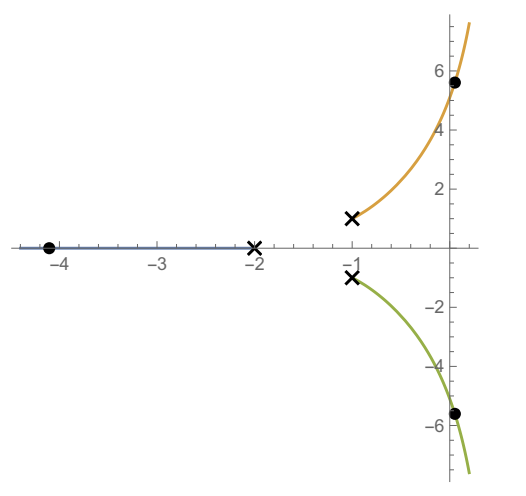
\includegraphics[scale=0.5]{figs/7.2.png}
    \caption{All poles and zeros in LHP and still high gain can make a system unstable.}
    \label{fig:prb_6}
\end{figure}
\textbf{\textcolor{red}{Solution :}} 
\begin{itemize}
    \item [(a)] Although, all poles and zeros are in the LHP, it does not necessary mean that all values of gain, K, will keep the system stable. Suppose that the transfer function is strictly proper, then the asymptotes should be taken into consideration. If there are $j \omega$-crossings, then some asymptotes may escape into RHP with high gain, causing the system to be unstable (see Fig. \ref{fig:prb_6}). For example, consider a system with a zero at $s =-5$ and poles at $s =-2, s =-1 \pm j$. Although, it has 3 LHP poles and 1 LHP zero, the root locus plot of this system shows that there are $j \omega$-crossings and the system becomes unstable with high gain.
    \item[(b)]  Root locus branches start at the poles and end at the zeros. If the number of poles is greater than the number of zeros, then some branch(es) will go to infinity. In this case, there is one unstable pole (RHP pole). Since there are equal numbers of poles and zeros, all branches will end at the zeros and because all the zeros are in the LHP, a large enough K can stabilize the closed-loop system.
    \item[(c)] Similar to the previous problem, all branches will start at the poles and end at the zeros. This case also has equal number of both. However, one of the zeros is in the RHP. Therefore, a large value of K can cause the closed-loop system to be unstable. 
\end{itemize}
\clearpage

\subsection{Minimizing Performance Index}

Consider the system

\begin{equation}
\begin{split}
    \dot{x}_1 &= x_1 + x_2 \\
    \dot{x}_2 &= - x_1 + x_2 + u \\
    y &= 2x_1 + x_2  \\
\end{split}
\end{equation}
and suppose that the control objective is to minimize the performance $ \int_0^\infty [\rho y^2(t) + u^2(t)]dt \quad  \rho> 0$.
\begin{itemize}
    % \item [(a)] Show graphically the locations of the optimal closed-loop poles as the parameter $\rho$ varies (symmetric root locus).
    \item [(a)] See why in the limit as $\rho \rightarrow 0$ (“expensive control” case), the optimal closed-loop poles become mirror images of the open-loop poles across the imaginary axis.
    \item [(b)] See why in the limit as  $\rho \rightarrow \infty$(“cheap control” case), one optimal closed-loop pole cancels the open-loop zero and the other moves off to $-\infty$.
\end{itemize}
\textbf{\textcolor{red}{Solution :}} \\

\begin{figure}[H]
    \centering
    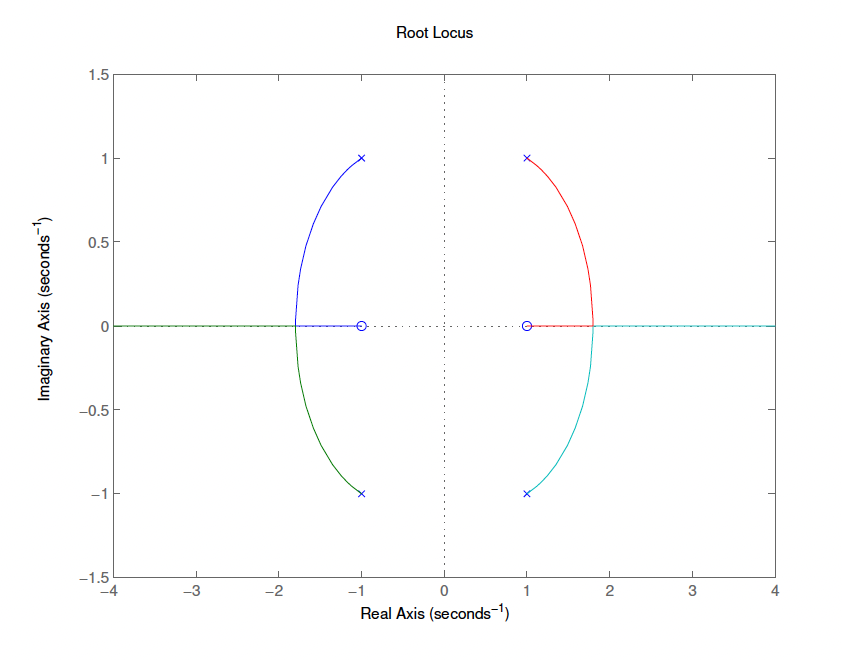
\includegraphics[width=0.5\linewidth]{figs/7.3.png}
    \caption{Root Locus of the system}
    \label{fig:prb18}
\end{figure}

\begin{equation*}
    \begin{split}
        \dot{x} &=\bmat{1 & 1\\ -1 &1} x +\bmat{0\\1}u \\
        y&=\bmat{2 & 1}x
    \end{split}
\end{equation*}


\begin{itemize}
  
\item [(a)] open-loop poles: $1 \pm j$  from Fig. \ref{fig:prb18}, we see that for every $\rho$, we assign the LHP pole for the closed loop system (due to symmetry vs imaginary axis)
For $\rho=0$, the CL-optimal poles would be $-1 \pm j$ because the OL-poles are on RHP, it would be the mirror images of OL-poles across the imaginary axis (Note: if the OL-poles were on LHP, then CL-poles would be equal to OL poles in this case).
\item [(b)] For $\rho \rightarrow -\infty$, one pole moves to zero, the zero is on LHP, so it cancels the pole, and the other one goes to $- \infty$.

\end{itemize}
\clearpage

\subsection{PI Controller}

 Consider the approximate model of a DC motor is given as: $$G(s)=\frac{.5}{(.01 s+1)(.1 s+1)}$$
 Design a PI controller such that it meets the following specifications: $$\zeta \geq 0.6,\left.\quad e_{s s}\right|_{\text {step }} \leq 0.01$$.
 \textbf{\textcolor{red}{Solution :}} \\
 \begin{figure}[h!]
     \centering
     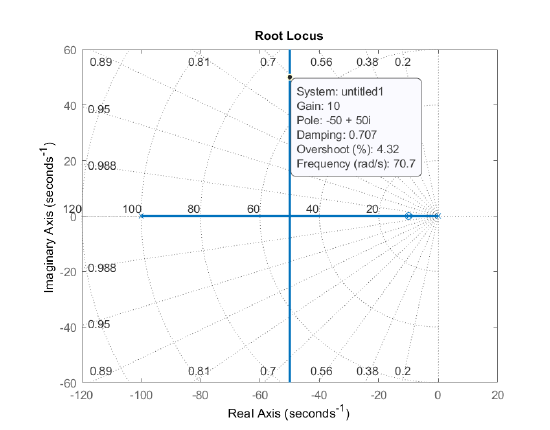
\includegraphics[width=0.75\linewidth]{figs/7.4.png}
     \caption{Root Locus Plot for the PI Controller.}
     \label{fig:prb19}
 \end{figure}
We choose a PI controller, $K(s)=\frac{K\left(s+z_c\right)}{s}$, with unity-gain feedback $H(s)=1$. The loop gain is given as: 
$$K(s) G(s)=\frac{.5 K\left(s+z_c\right)}{s(.01 s+1)(.1 s+1)}$$
The position error constant is $K_p=\infty$. Hence $\left.e_{s s}\right|_{\text {step }}=0$.
The controller zero can be selected to cancel one of the plant poles; hence $z_c=10$. Next, from the Root Locus plot given in Fig. \ref{fig:prb19}, we may choose, e.g., $K=10$. The PI controller design is given as: $$K(s)=\frac{10(s+10)}{s}$$
The closed-loop system transfer function is thus given by $T(s)=\frac{5000}{s^2+100 s+5000}$. 

\clearpage

\subsection{Phase-Lag Controller}

Consider the following system:
$$G(s)=\frac{10}{s(s+2)(s+5)}$$ 
Design a Phase-Lag controller such that it meets the following design specifications: 
$$\zeta \geq 0.6,\left.\quad e_{s s}\right|_{\mathrm{ramp}} \leq 0.1$$

\textbf{\textcolor{red}{Solution :}} \\
Since transient response improvement is not aimed, we may use a static controller to satisfy the damping ratio requirement. Let $K=0.7$; then, the closed-loop system has dominant roots at: $s=-0.8 \pm j 0.8(\zeta=0.7)$. The characteristic polynomial is factored as: 
$$\Delta(s)=(s+5.38)\left(s^2+1.62 s+1.3\right)$$

Next, the velocity error constant is evaluated as: $K_v=0.7$. In order to raise $K_v>10$, we consider a phase-lag controller: $K(s)=\frac{s+0.02}{s+0.0012}$, where $\angle K\left(s_1\right)=-0.3^{\circ}$. The compensated system has: $K_v=11.67$; hence $\left.e_{s s}\right|_{\text {ramp }} \leq 0.1$. The ramp response of the closed-loop system is plotted to confirm the results.


\begin{figure}[H]
    \centering
    \begin{subfigure}[b]{0.45\textwidth}
    \centering
    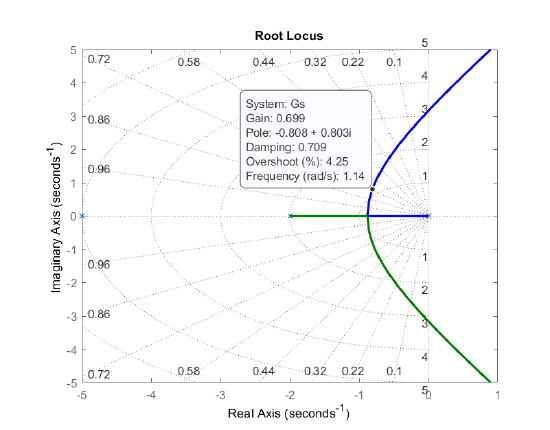
\includegraphics[width=\textwidth]{figs/7.5-1.png}
     \caption{Root locus plot for phase-lag design}
     \end{subfigure}
     \begin{subfigure}[b]{0.45\textwidth}
     \centering
        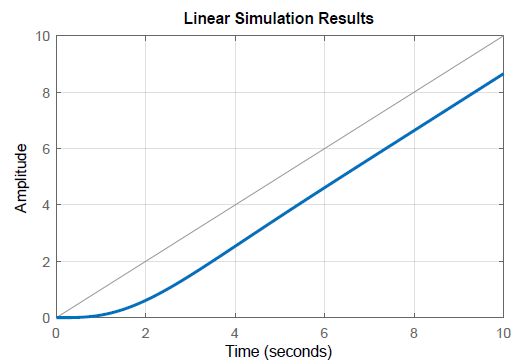
\includegraphics[width=\textwidth]{figs/7.5-2.png}
     \caption{ Closed-loop system response}
     \end{subfigure}
    \caption{Root Locus and Response of the Systems}\label{fig:prb20}
\end{figure}

\noindent With the addition of the phase-lag controller, the closed-loop transfer function is given as:
$$
T(s)=\frac{7(s+0.02)}{(s+0.0202)(s+5.38)\left(s^2+1.61 s+1.29\right)}
$$

The closed-loop root at $s=-0.0202$ is almost canceled by the presence of the zero at $s=-0.02$. Hence, the slow mode $e^{-0.0202 t}$ has a very small coefficient and only minimally affects the system response. The dominant closed-loop roots are also minimally affected.
\clearpage

\subsection{Overshoot}

Consider the system 
\[
G(s)=\frac{s + 2}{(s+1)^2 +1}
\]
The positive root locus for $G(s)$ is given in Fig. \ref{fig:prb38}.Suppose you want to find a feedback gain that is a positive integer $(K = 1, 2, 3, \hdots )$ such that the
closed-loop system has overshoot $M_p$ as small as possible and settling time ts is as fast possible. Explain what value of K you would pick and why?\\
\begin{figure}[H]
    \centering
    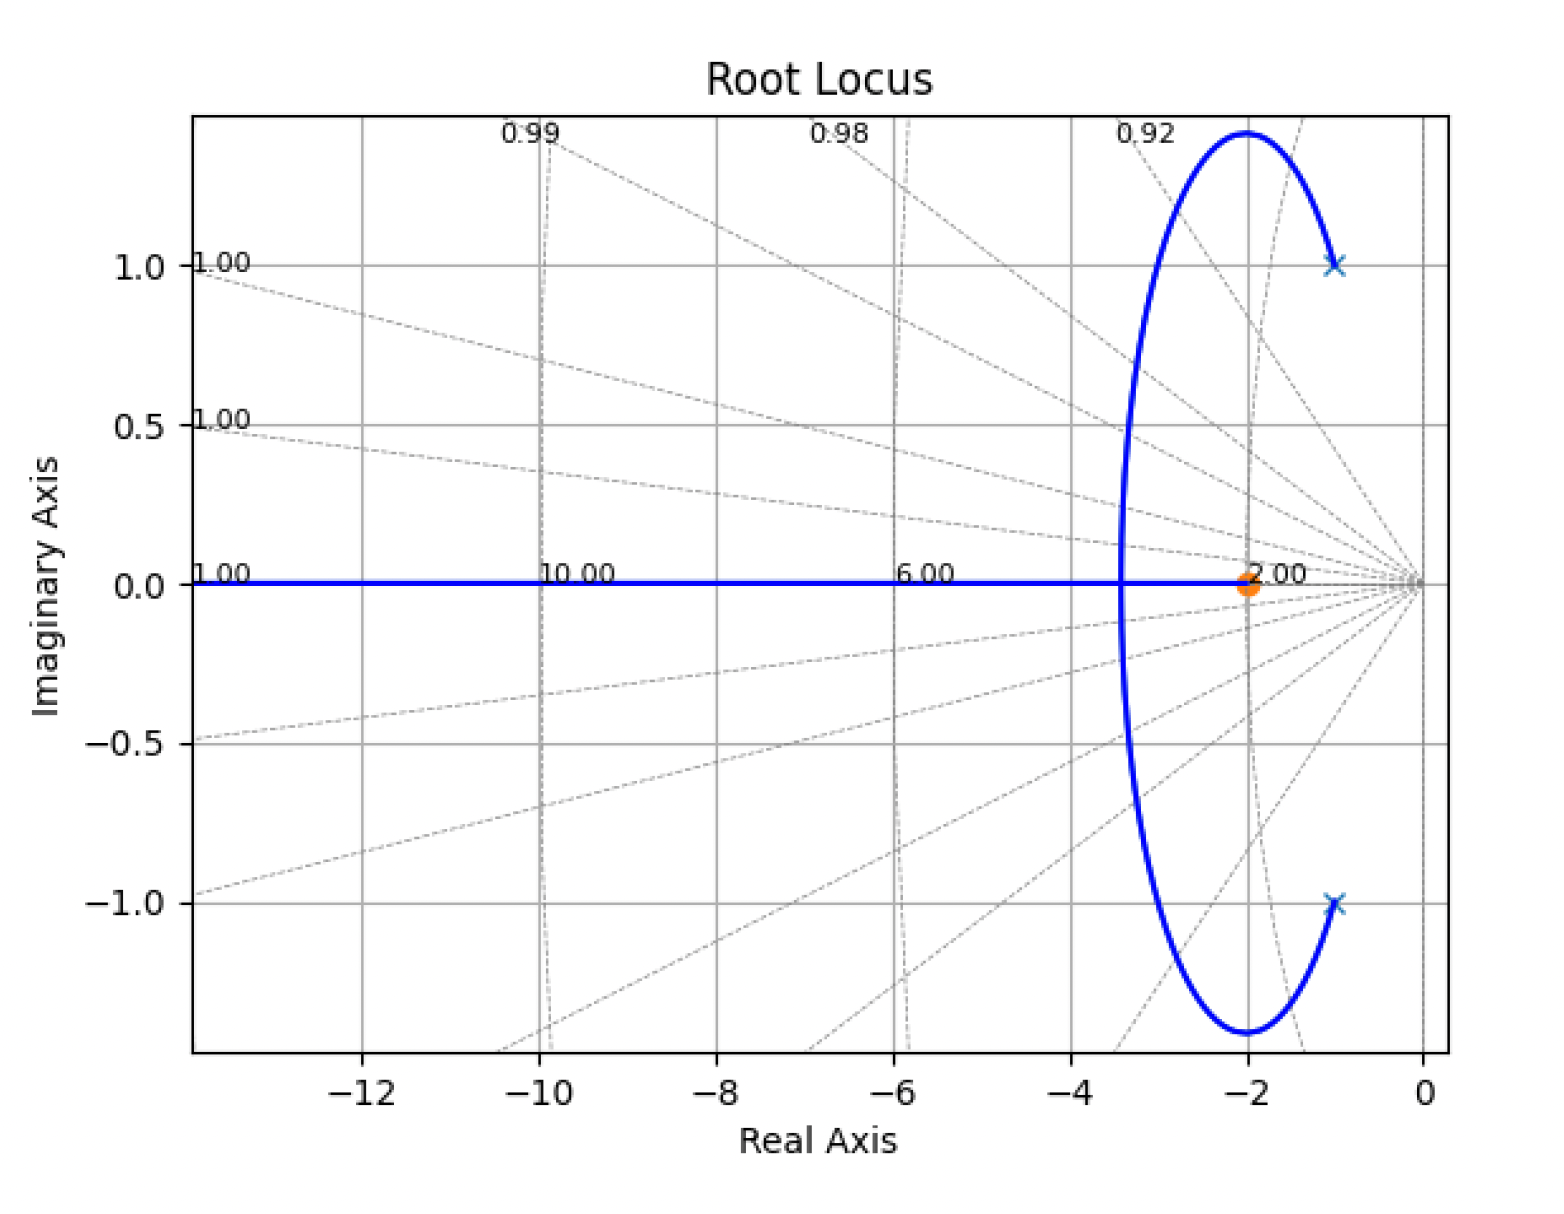
\includegraphics[width=0.6\linewidth]{figs/7.6.png}
    \caption{Root Locus of the System}
    \label{fig:prb38}
\end{figure}
\textbf{\textcolor{red}{Solution :}} \\
Referring to the root locus in Fig. \ref{fig:prb38}. The best location for closed-loop poles is at $-2-\sqrt{2}$, the point of multiple roots, because negative real roots means no overshoot. For large K, one pole moves right towards -2, which is not good for settling time. Thus, closed-loop characteristic equation is $(s+2+\sqrt{2})^2$ and it also equals to $s^2+(K+2)s+2(K+1)$. We finally get $K = 2 + 2+\sqrt{2}$ and the nearest integer is K = 5.\\ 
\clearpage

\subsection{Stability Analysis}

Consider a feedback control system under unity feedback setting with a controller $K(s)=K$ and the system $G(s)$ given as follows:
\[
G(s)=\frac{s(s+10)(s+12)}{(s-1)(s+11)(s+13)(s+14)}
\]
Is there a non-negative value of $K$ for which the closed loop system is stable? Explain why or why not?\\

\textbf{\textcolor{red}{Solution :}} \\
No, there is no non-negative value of $K$ for which the closed loop system is stable. Check the root locus given below. The root locus branch between the RHP pole and the imaginary axis zero keeps the system unstable. 

\begin{figure}[h!]
    \centering
    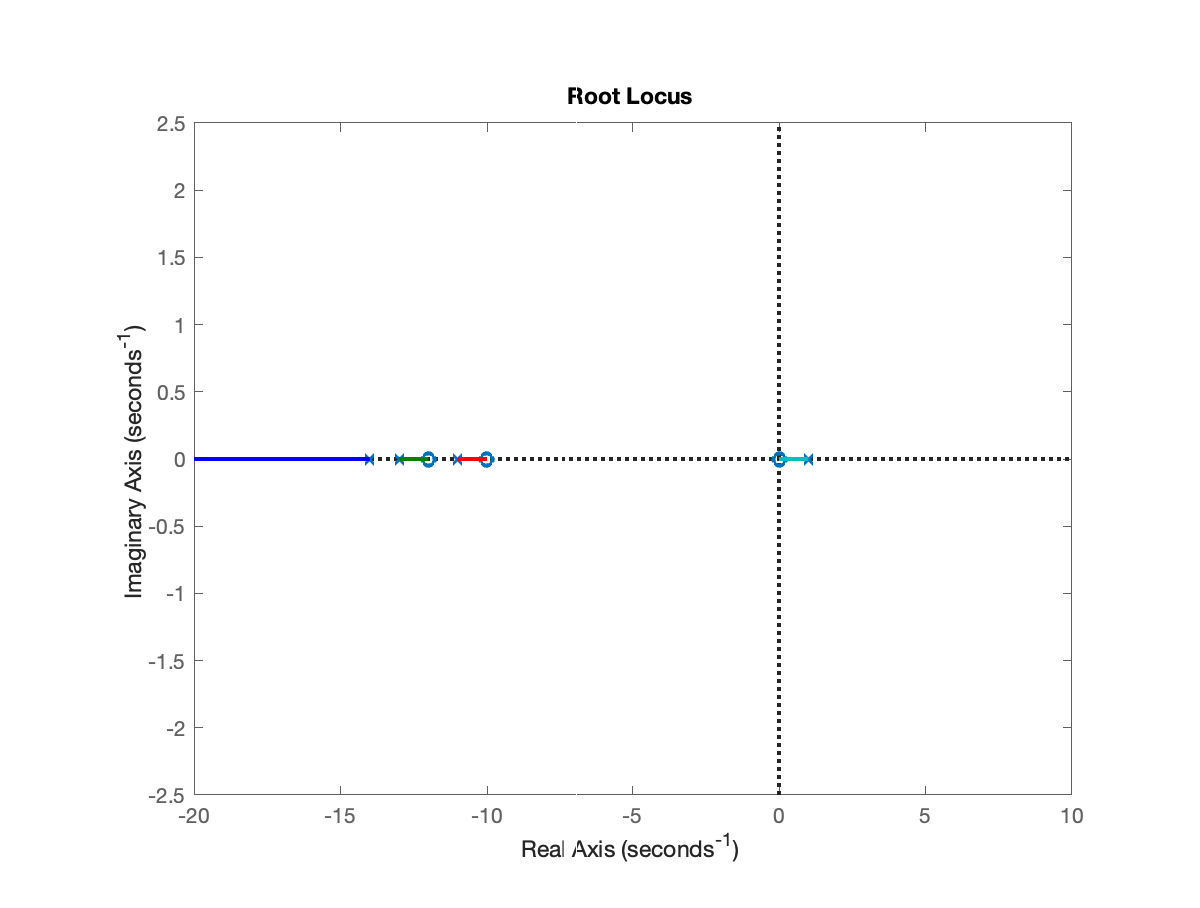
\includegraphics[width=0.75\linewidth]{figs/7.7.eps}
    \caption{Root Locus of G(s)}
    \label{fig:prb46}
\end{figure}
\clearpage

\section{Nyquist Design}
\subsection{Nyquist Stability Analysis}

Consider a standard closed-loop system characterized by the loop transfer function $L(s)$. The stability of the closed-loop system can be predicted by applying the Nyquist stability criterion, which involves analyzing the Nyquist plots of $L(s)$. Below are the Nyquist plots for two different loop transfer functions, labeled as (a) and (b). Use the Nyquist stability theorem to determine the number of poles in the right-half plane (RHP) for the closed-loop system based on these plots. Then, classify each system as either stable or unstable.

\[
\begin{minipage}{0.5\textwidth}
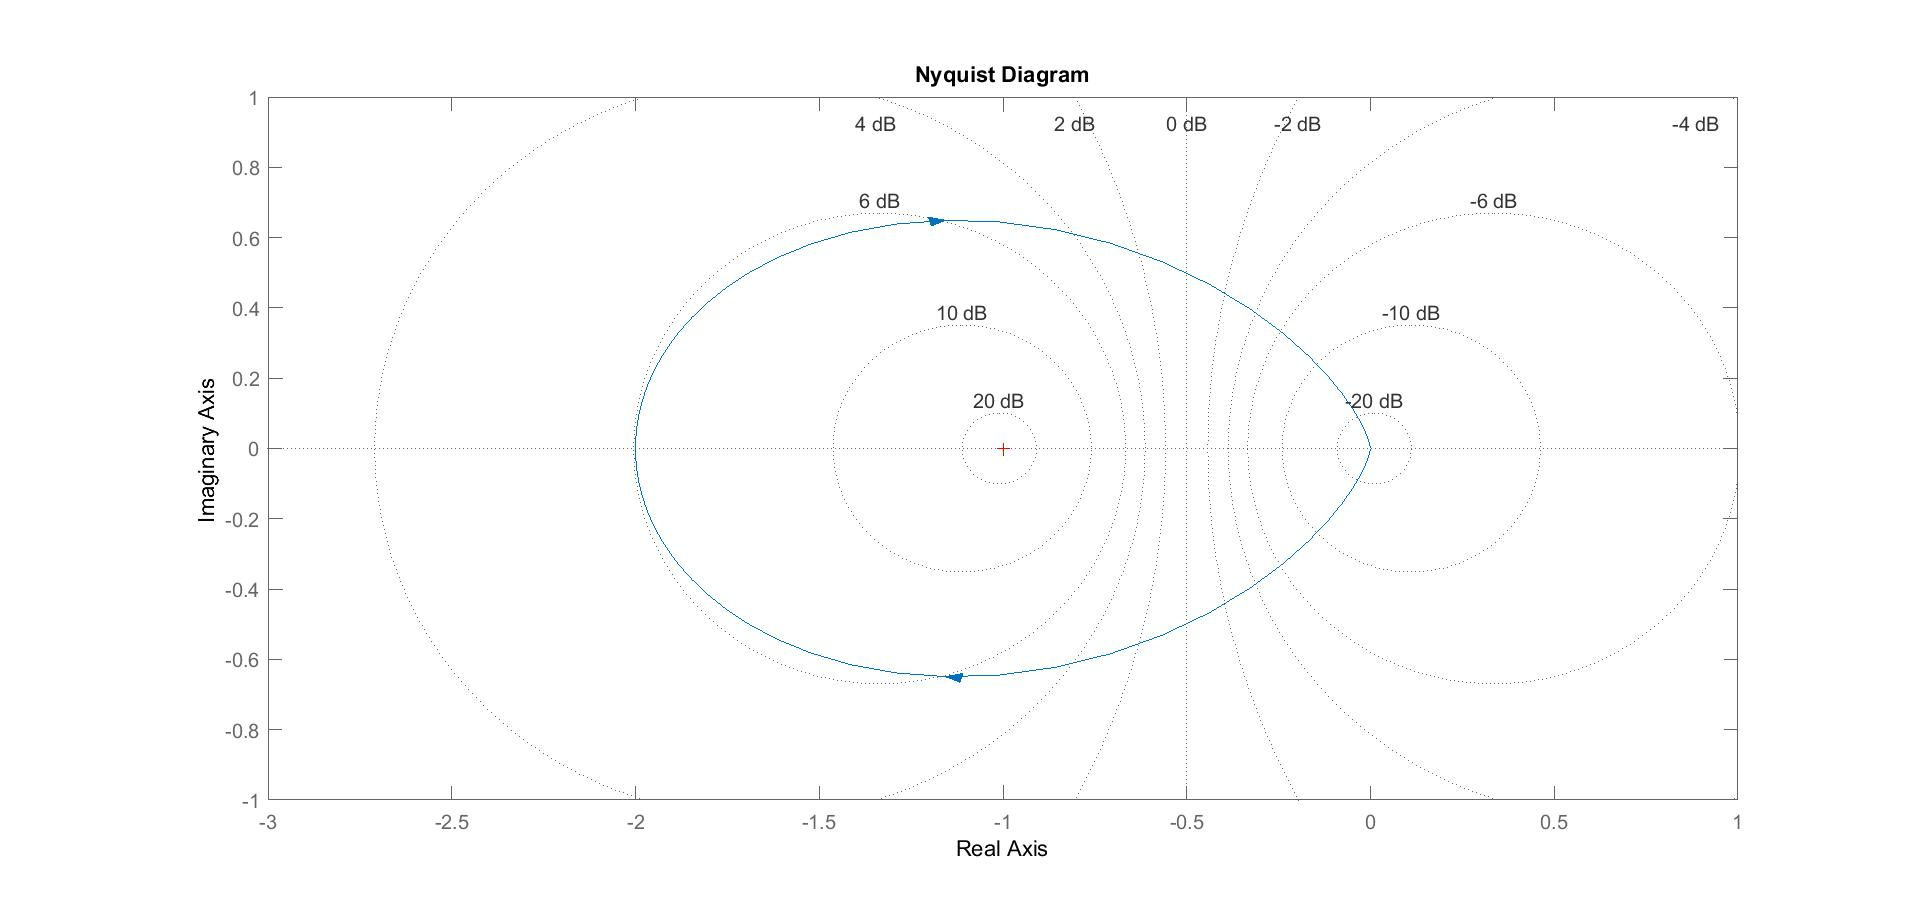
\includegraphics[width=\linewidth]{figs/8.1-a.jpg}
\centering
\text{(a) Nyquist Plot for $L(s)$ in scenario (a)}
\end{minipage}%
\begin{minipage}{0.5\textwidth}
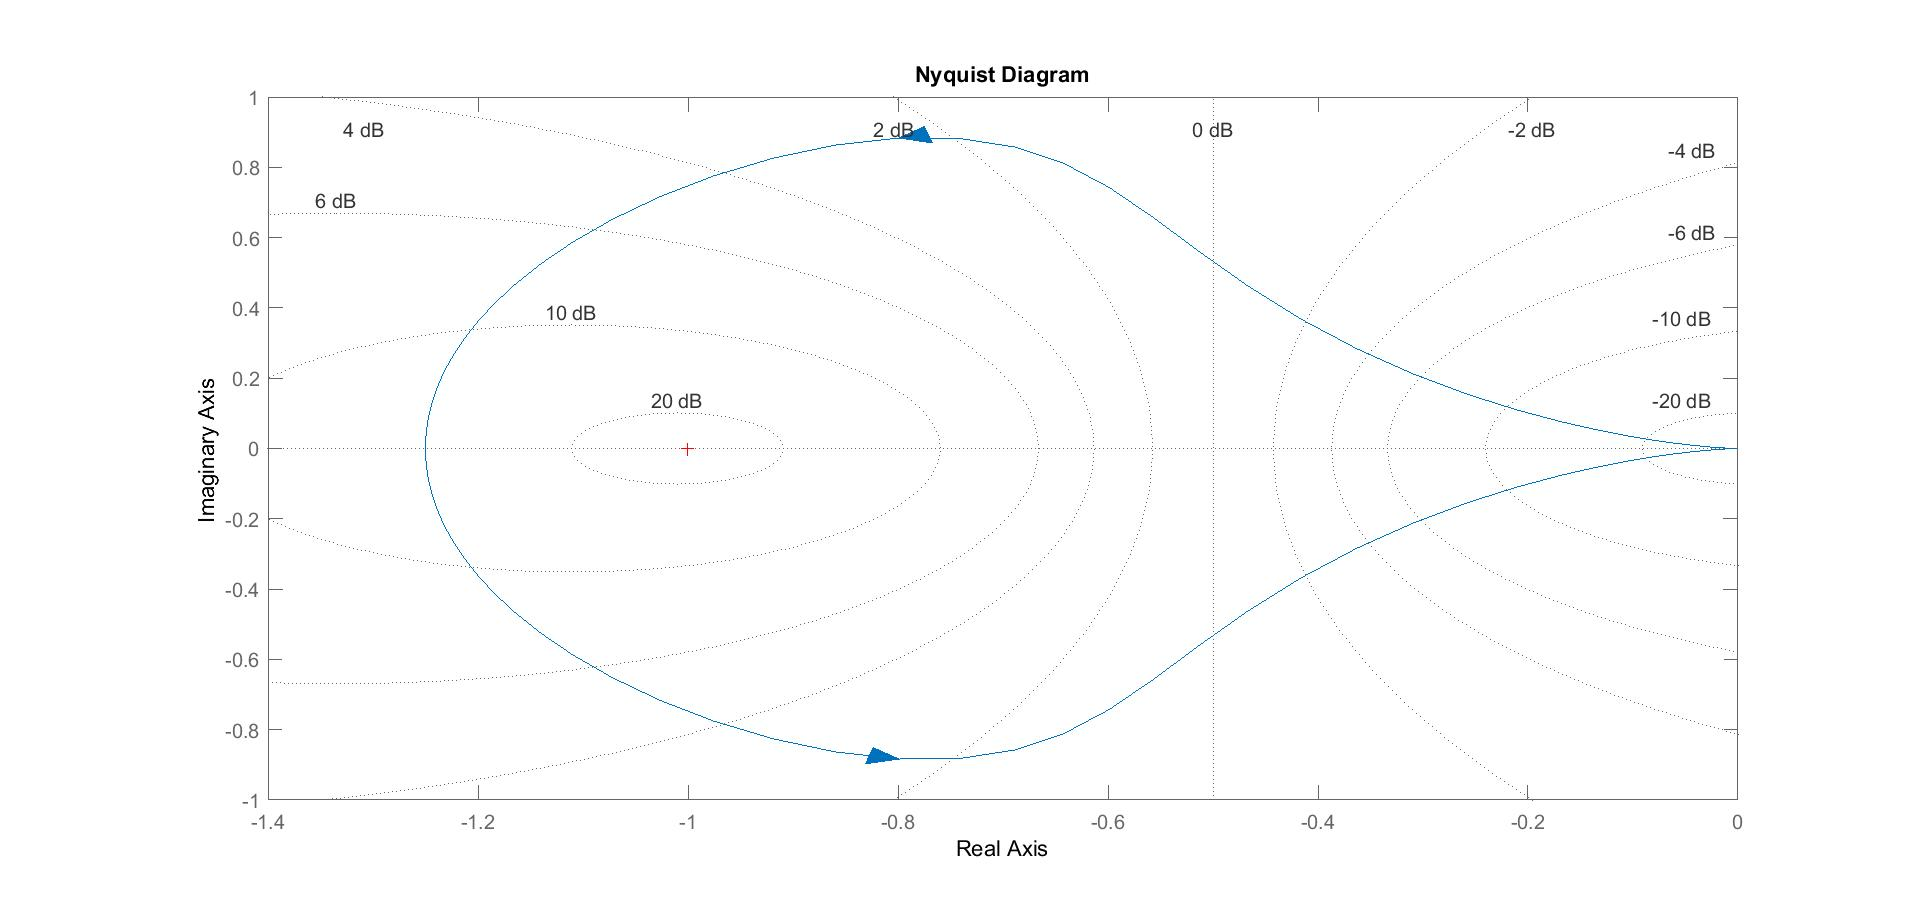
\includegraphics[width=\linewidth]{figs/8.1-b.jpg}
\centering
\text{(b) Nyquist Plot for $L(s)$ in scenario (b)}
\end{minipage}
\]

\textbf{\textcolor{red}{Solution :}} \\
\begin{itemize}
    \item[(a)] Unstable. \\
    Steps: $P_{CL} = P_{OL} - N_{CCW} = 1 - (-1) = +2.$
    \item[(b)] Stable. \\
    Steps: $P_{CL} = P_{OL} - N_{CCW} = 1 - 1 = 0.$
\end{itemize}
\clearpage

\subsection{State-Feedback Controller Design and Stability Analysis}

Consider the single-input, single-output transfer function:
$$G_p(s) = \frac{1-s/2}{s^2 (1+s/2)}$$
\begin{itemize}
    \item[(a)] Calculate a state-feedback controller $u = - K x + r$ that places the closed loop poles at -4, -13 and -25.
    \item[(b)] Construct a stable observer and put this together to form a compensator of the form $U=-G_c Y + G_r R$.
    \item[(c)] Calculate the Nyquist plot of $G_cG_p$. Is the system stable? If so, calculate the gain and phase margins.
\end{itemize}
  

\textbf{\textcolor{red}{Solution :}} \\
We can place the closed loop poles at the desired locations using the gain $K =\bmat{1300 & 477 & 40}$. Suppose we place the observer poles at -50, -51, -52 which leads to the observer gain  $$L =\bmat{ 9301 & 18450 & 29400}^T $$ The transfer functions $G_c$ and $G_r$ are thus given as follows:
\begin{align*}
    G_c &=\frac{2.207e07 s^2 + 7.979e07 s + 8.619e07}{s^3 + 193s^2 + 1.432e04s + 2.257e07} \\
    G_r &= \frac{s^3 + 153s^2 + 7802s + 1.326e05}{s^3 + 193s^2 + 1.432e04s + 2.257e07}
\end{align*}

The Nyquist plot of $G_cG_p$ is given in Fig. \ref{fig:prb_4a}. 
\begin{figure}[H]
    \centering
    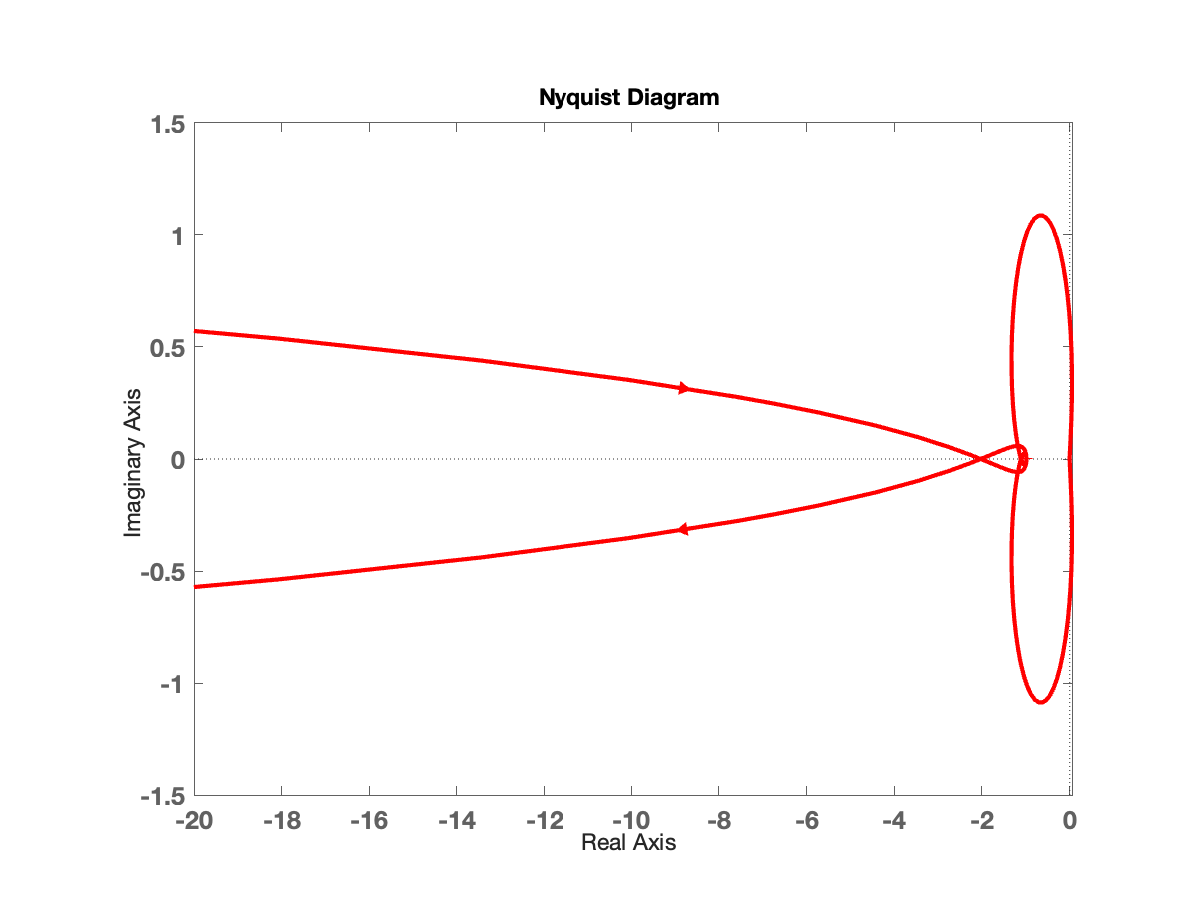
\includegraphics[scale=0.6]{figs/8.2-1.eps}
    \caption{Nyquist Plot of $G_cG_p$}
    \label{fig:prb_4a}
\end{figure}

 The gain margin is 0.115 dB and the phase margin is -1.11 deg. We now check stability with the nyquist plot. We will use Fig. \ref{fig:prb_4b} for counting the number of windings around -1. Clearly there are 3 anticlockwise loops around -1, coloured in red, green and blue. So N must be -3. Gc has 2 RHP poles, and $G_p$ has 2 poles at origin. If the poles at origin are included as RHP poles, P = 4, else P = 2. In either case, $Z = N + P = 1/ -1$ and not zero. However, the closed loop has to be stable because we placed the poles in the LHP ourselves. 

 \begin{figure}[H]
    \centering
    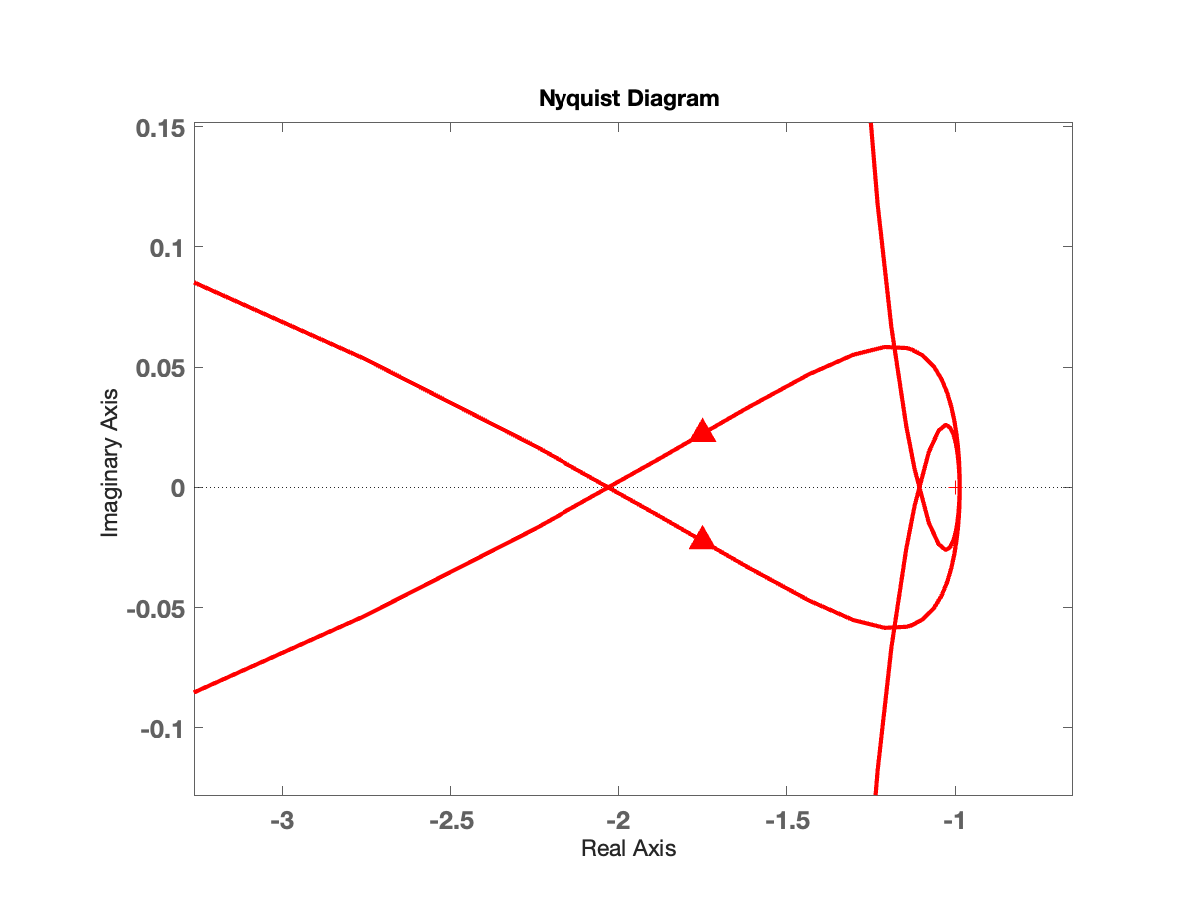
\includegraphics[scale=0.6]{figs/8.2-2.eps}
    \caption{Stability check}
    \label{fig:prb_4b}
\end{figure}


The problem here is that $G_c$ has a double pole at the origin. This is why the Nyquist plot
is not a closed loop, and shoots to infinity as $\omega$ approaches zero. So we need to consider a small semi-circular modified contour of radius r around the origin. Radius r is taken to be very small. There are three poles in $G_c$, two of which are in RHP and one is in LHP. There are three poles in $G_p$ as well, one in LHP and two at the origin. However, with respect to the modified contour, the two poles at the origin lie in the LHP. So they are not counted as open loop RHP poles and P = 2.

Now we need to understand how the image of the Nyquist plot changes under this modified contour. We forget the 3 anticlockwise loops already accounted for before and focus only on the part that shoots off to infinity in Fig. \ref{fig:prb_4b}. For r very small, $G_p G_c\left(j r \right) \approx  \frac{k}{(jr)^2} = - \frac{k}{r^2}$  where k is the finite limit $\lim s \rightarrow 0 s^2 G_c G_p(s)$. The point is that $G_cG_p(jr)$ will be close to the real line even though its magnitude is very large $\approx \frac{k}{r^2}$. Since the plot goes toward negative infinity, we can also say that k is negative. The semicircular contour can be parameterized as $r e^{j\theta}$ as $\theta$ goes from $ - \frac{\pi}{2} \rightarrow  - \frac{\pi}{4} \rightarrow 0 \rightarrow \frac{\pi}{4} \rightarrow \frac{\pi}{2}$. Since r is really small, $G_cG_p(re^{j\theta}) \approx -\frac{k}{r^2}e^{-2j\theta}$. Since $-k$ is positive, the phase of $G_cG_p(re^{j\theta})$ will be $\approx e^{-2 j \theta}$. As $\theta$ travels from $-\frac{\pi}{2}$ to $\frac{\pi}{2}$ in the anti-clockwise direction, $-2\theta$ travel from $-\pi$ back to $\pi = - \pi $ in the clockwise direction. So the Nyquist plot travels through a large clockwise circle of radius $-\frac{k}{r^2}$ when we modify the contour. This circle will wind around -1 due to its very large radius, which makes $N =-3+1=-2$. Since $P = 2$, $Z = N + P = 0$ which means the system is stable.
\clearpage

\subsection{Stabilizing Controllers}

Consider the following:
$$G(s) =\frac{1}{(s + 2)(s2 + 2s + 5)}$$
Suppose this is in unity feedback with a constant gain controller K. In other words, we have a
negative feedback loop where the forward gain is KG(s) and the loop gain is also KG(s). 
\begin{itemize}
    \item [(a)] Determine what values of K stabilize the closed-loop system using the Routh-Hurwitz stability criterion. 
    \item [(b)] Using the Nyquist plot, determine what values of K stabilize the closed-loop system. Does this match your answer from the Routh-Hurwitz criterion?
\end{itemize}
    \begin{figure}[h!]
        \centering
        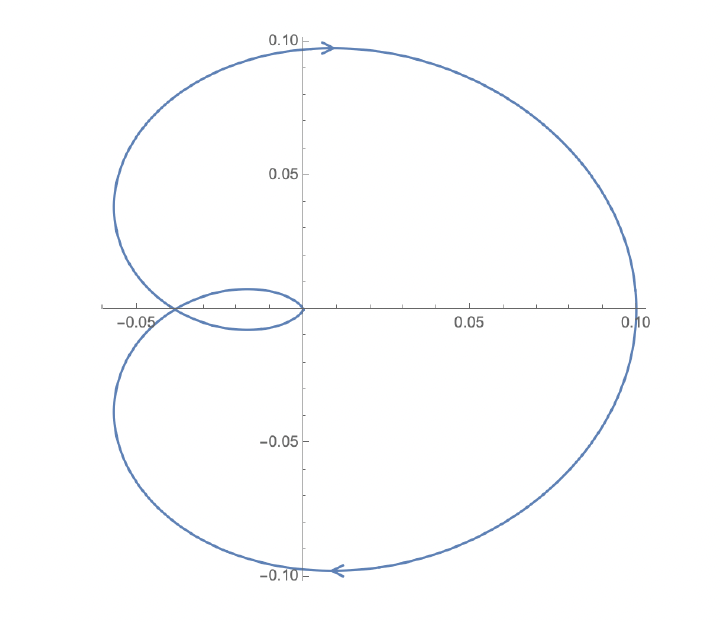
\includegraphics[width=0.5\linewidth]{figs/8.3.png}
        \caption{Nyquist plot of the system}
        \label{fig:prb12}
    \end{figure}

\textbf{\textcolor{red}{Solution :}} 
\begin{itemize}
    \item [(a)] The characteristic equation is: $s^3 + 4s^2 + 9s + 10 + K$ and the Routh table reads as follows and it yields that $-10 < K < 26$.
    \begin{table}[h!]
        \centering
        \begin{tabular}{c c c}
            $s^3$ &  1 & 9 \\
            $s^2$ &  4 & 10+K\\
            $s^1$ &  $-\frac{1}{4}(K-26)$ & 0\\
            $s^0$ & K+10 & 
        \end{tabular}
    \end{table}


    \item[(b)] Fig. \ref{fig:prb12} shows the Nyquist plot for this system. Let N be the number of encirclements of $\frac{-1}{K}$ and P be the number of open loop poles. We have that $N = Z - P$ where Z is the number of closed loop poles. In this particular case P = 0 yielding N = Z. This gives that
$$- \frac{1}{K}> 10 \qquad - \frac{1}{K}<0.0384$$
which is the same condition as derived using Routh-Hurwitz criterion.
\end{itemize}
\clearpage

\subsection{Gain/Phase Margin}

Use the Nyquist plot of KG(s) to calculate the gain margin and phase margin for the following system $G(s)$ and controller $K(s)$:
$$G(s)=\frac{1}{(s + 1)(s + 2)(s + 4)} \qquad K=10$$
Assume the system and the controller are in standard unity feedback setting. \\

\begin{figure}[H]
    \centering
    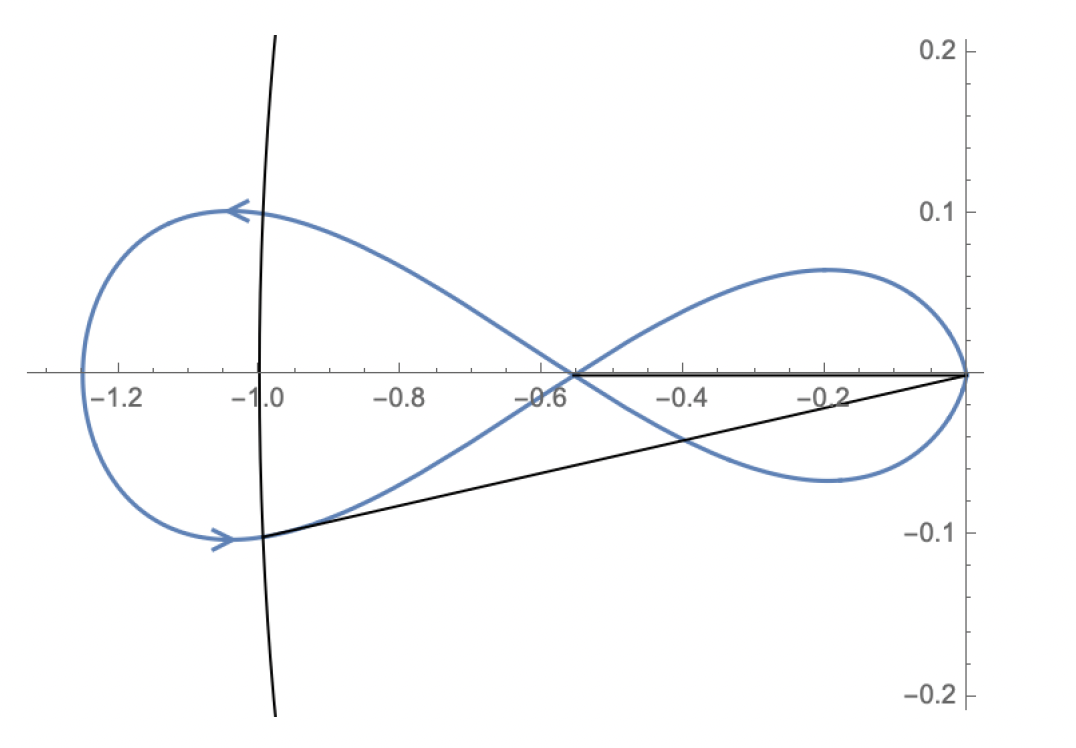
\includegraphics[width=0.5\linewidth]{figs/8.4.png}
    \caption{Nyquist Plot of the System}
    \label{fig:prb13}
\end{figure}
\textbf{\textcolor{red}{Solution :}} \\
Nyquist plot of KG(s) is shown in Fig. \ref{fig:prb13}. From the Nyquist plot, two points (-0.55, -1.25) intersect the negative real axis. The
corresponding gain margins are $\frac{1}{0.55} \approx 1.8$ and $\frac{1}{1.25} \approx 0.8$. The GM of the system is $[0.8,1.8]$.

To obtain PM from the Nyquist plot, draw a unit circle and mark the points where unit
circle intersects the Nyquist plot. Draw a line from the origin to one of the points. The
angle formed between that line and the $180^\circ$ axis is the PM. The Nyquist plot here
intersects the unit circle at two symmetric points, one of which is $\approx(-0.995, -0.1)$ and
so the PM is $\arctan\left( \frac{-0.1}{-0.995}\right)= 5.74$ degrees.
\clearpage

\subsection{Closed-Loop Poles of the Feedback}

Consider the system $G(s)$ and the controller $K(s)$ are in standard unity feedback setting. Define $L(s) := G(s)K(s)$. Use the Nyquist plot for the following loop transfer functions and apply the Nyquist stability theorem to predict the number of closed-loop poles of the feedback system in the right-half plane.
$$(a) \quad L(s)=\frac{-8}{s+4} \qquad \qquad  (b) \quad L(s)=\frac{2s +9}{s-4}$$
\textbf{\textcolor{red}{Solution :}} \\

\begin{figure}[H]
    \centering
    \begin{subfigure}[b]{0.45\textwidth}
    \centering
    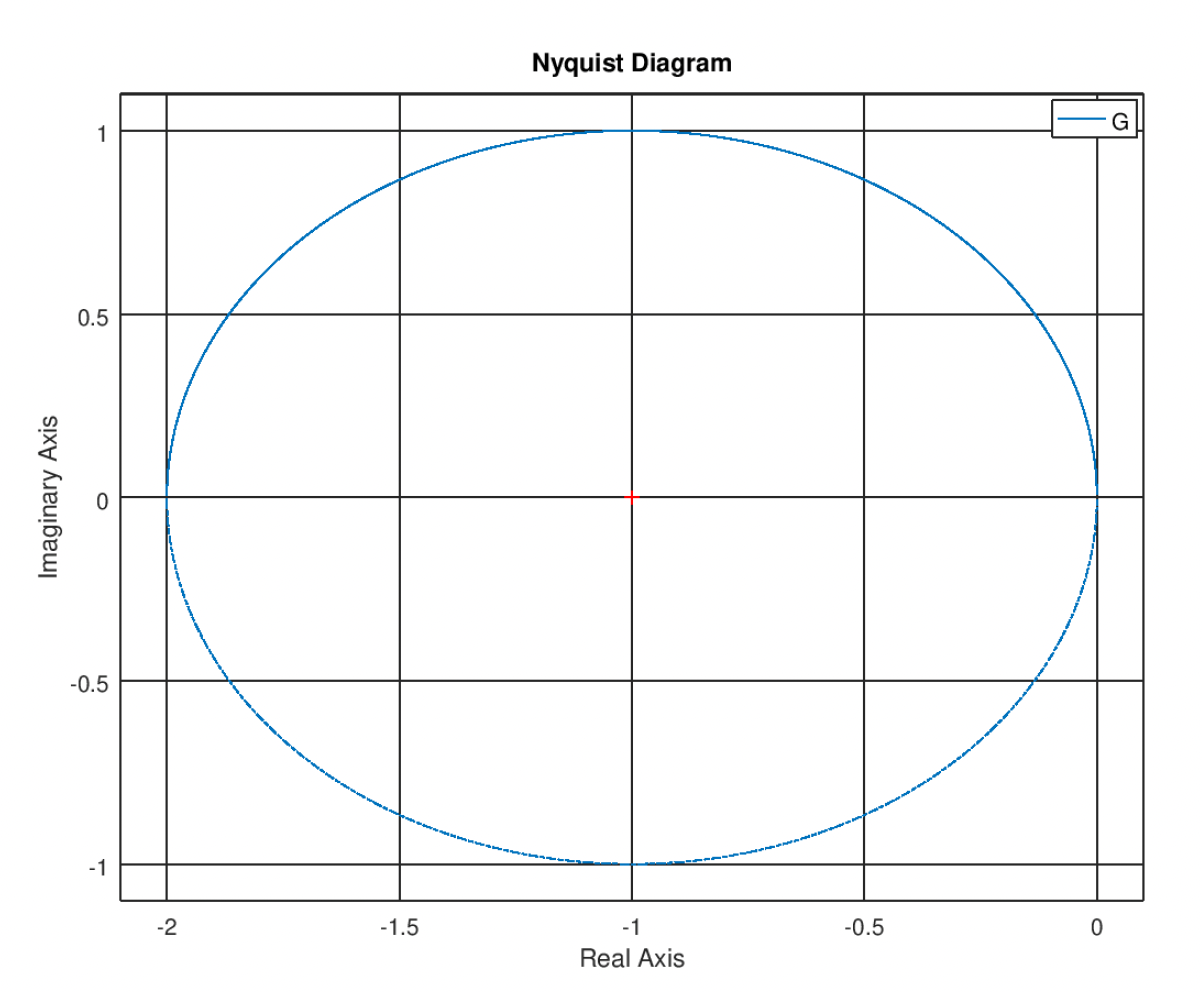
\includegraphics[width=\textwidth]{figs/8.5-1.png}
     \caption{Nyquist Plot of $L(s)$ in (a)}
     \end{subfigure}
     \begin{subfigure}[b]{0.46\textwidth}
     \centering
        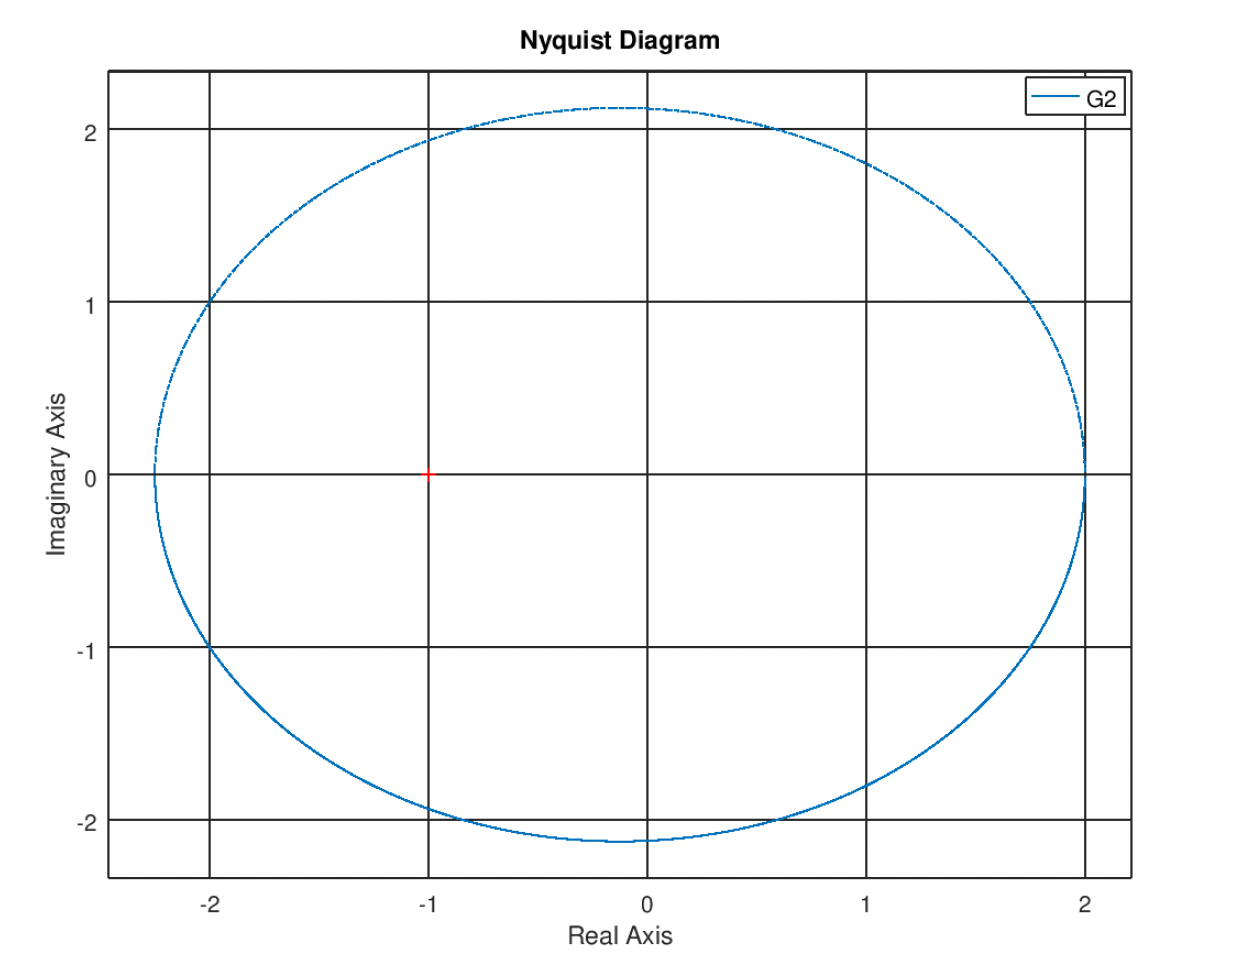
\includegraphics[width=\textwidth]{figs/8.5-2.png}
     \caption{Nyquist Plot of $L(s)$ in (b)}
     \end{subfigure}
    \caption{Nyquist Plot for the Systems}\label{fig:prb14}
\end{figure}

The Nyquist plot for the two $L(s)$ is given in Fig. \ref{fig:prb14}.The Nyquist stability theorem says that if the number of RHP poles of the closed loop transfer function $\frac{L(s)}{1+L(s)}$ is Z, the number of RHP poles of the open loop transfer function L(s) is P, and N is the number of clockwise rotations of the Nyquist plot around -1, then Z = N + P. Therefore,
    \begin{itemize}
        \item [(a)] N = 1; P = 0 so Z = 1.
        \item [(b)] N = -1; P = 1 so Z = 0.
    \end{itemize}
\clearpage

\section{Gain/Phase Margins}
\subsection{Gain/Phase Margins}

Determine the gain and phase margin for the system in which \(GH(j\omega) = \frac{1}{(j\omega+1)^3}\)

\textbf{\textcolor{red}{Solution :}} \\
Writing $GH(j\omega)$ in polar form, we have
\begin{itemize}
    \item The magnitude $|GH(j\omega)| = \frac{1}{\sqrt{\omega^2 + 1}^3}$
    \item The phase $\angle GH(j\omega) = -3 \tan^{-1}(\omega)$
\end{itemize}
Then \(-3 \tan^{-1} \omega_\pi = -\pi, \omega_\pi = \tan(\pi/3) = \sqrt{3}\). Hence, gain margin is
\[ \frac{1}{|GH(j\omega_\pi)|} = 8\]
Also,
\[|GH(j\omega_1)| = \frac{1}{(\omega_1^2+1)^{3/2}} = 1\]
happens only at \(\omega_1  = 0\), therefore
\[\phi_{PM} = 180^\circ + (-3\tan^{-1} 0) = 180^\circ = \pi \quad  \text{radians}\]
\clearpage

\subsection{Bandwidth}

Determine the bandwidth for the system with transfer function \((C/R)(s) = 1/(s+1)\).

\textbf{\textcolor{red}{Solution :}} \\
we have
\begin{equation}
    \left|\frac{C}{R}(j\omega)\right| = \frac{1}{\sqrt{\omega^2+1}}
\end{equation}
The bandwidth is the frequency at which this magnitude drops to \(\frac{1}{\sqrt{2}}\) of its maximum value. Since  \(|(C/R)(j\omega)|\) is a strictly decreasing function of positive frequency,  maximum happens at \(\omega = 0\). Setting the magnitude equal to \(\frac{1}{\sqrt{2}} \times \frac{1}{\sqrt{0+1}} \) and solving for \(\omega\) yields:

\[ \frac{1}{\sqrt{\omega^2 + 1}} = \frac{1}{\sqrt{2}} \]

Solving this equation:

\[ \sqrt{\omega^2 + 1} = \sqrt{2} \]
\[ \omega^2 + 1 = 2 \]
\[ \omega^2 = 1 \]
\[ \omega = 1 \]
Therefore, the bandwidth of the system is \(\omega = 1\) rad/s.
\clearpage

\subsection{Resonance Peak}

Determine the resonance peak \(M_p\) and the resonant frequency \(\omega_p\) for the system whose transfer function is \(\frac{C}{R}(s) = \frac{5}{s^2 + 2s + 5}\).

\textbf{\textcolor{red}{Solution :}} \\
The magnitude \(|C/R(j\omega)|\) is given by:

\[
\left| \frac{C}{R}(j\omega) \right| = \left| \frac{5}{- \omega^2 + 2j\omega + 5} \right| = \frac{5}{\sqrt{\omega^4 - 6\omega^2 + 25}}
\]

Setting the derivative of \(\left| \frac{C}{R}(j\omega) \right|\) equal to zero, we get \(\omega_p = \pm \sqrt{3}\). Therefore,
\begin{equation}
    M_P = \max_\omega \left| \frac{C}{R}(j\omega) \right| = \left| \frac{C}{R}(j\sqrt{3}) \right| = \frac{5}{4}
\end{equation}
\clearpage

\subsection{Gain/Phase Margins}

Calculate the gain and phase margin for \(GH = \frac{432}{s(s^2 + 13s + 115)}\).

\textbf{\textcolor{red}{Solution :}} \\
Given the open-loop transfer function \(GH(s) = \frac{432}{s(s^2 + 13s + 115)}\), we can write $GH(j\omega)$ in polar form
\begin{itemize}
    \item The magnitude $|GH(j\omega)| = \frac{432}{\sqrt{(115\omega-\omega^3)^2+(-13\omega^2)^2}}$
    \item The phase $\angle GH(j\omega) = - \tan^{-1}(\frac{115\omega - \omega^3}{-13\omega^2})$
\end{itemize}
Then \(- \tan^{-1}(\frac{115\omega_\pi - \omega_\pi^3}{-13\omega_\pi^2}) = -\pi, \omega_\pi =  \sqrt{115}\). Hence, gain margin is
\[ \frac{1}{|GH(j\omega_\pi)|} = \frac{13\times 115}{432} = 3.46\]
Also,
\[|GH(j\omega_1)| = \frac{432}{\sqrt{(115\omega_1-\omega_1^3)^2+(-13\omega_1^2)^2}} = 1\]
happens only at \(\omega_1  = 3.86\), therefore
\[\phi_{PM} = 180^\circ  - \tan^{-1}\left(\frac{115\omega_1 - \omega_1^3}{-13\omega_1^2}\right) = 64^\circ \]

\clearpage
\subsection{Gain Margin}

True or False:
\begin{itemize}
    \item[(a)] The gain margin is the amount of allowable variation in the phase of the plant before the closed loop becomes unstable.
    \item[(b)] As a rule of thumb (not being strict), the closed-loop should remain stable for gain variations in the range $[0.5, 2] (= ±6dB)$. 
    \end{itemize}
\textbf{\textcolor{red}{Solution :}} \\
\begin{itemize}
    \item[(a)] False. (should be the allowable variation in the gain of the plant) 
    \item[(b)] True. 
\end{itemize}

\clearpage
\subsection{Maximum Phase Lead}

Show that the maximum phase lead of the lead compensator
\begin{equation}
    P_{Lead}(j\omega) = \frac{(a/b)(1+j\omega/a)}{1+j\omega/b}
\end{equation}
occurs at \(\omega_m = \sqrt{ab}\) and find the maximum phase. What magnitude is produced at the maximum phase lead?

\textbf{\textcolor{red}{Solution :}} \\
The phase angle of the lead compensator is \(\phi = \arg P_{Lead}(j\omega) = \tan^{-1} \omega/a - \tan^{-1} \omega/b\). Then
\begin{equation}
    \frac{d\phi}{d\omega} = \frac{1}{a[1+(\omega/a)^2]} - \frac{1}{b[1+(\omega/b)^2]}
\end{equation}
Setting \(d\phi/d\omega\) equal to zero yields \(\omega^2 = ab\). Thus the maximum phase lead occurs at \(\omega_m = \sqrt{ab}\). Hence \(\phi_{\max} = \tan^{-1}\sqrt{b/a}-\tan^{1}\sqrt{a/b}\). But since \(\tan^{-1}\sqrt{b/a} = \pi/2-\tan^{-1}\sqrt{a/b}\), we have \(\phi_{\max} = (90 - 2\tan^{-1}\sqrt{a/b})\) degrees.

The magnitude factor is given by
\[|P_{Lead}(j\sqrt{ab})| = |\frac{(a/b)(1+j\sqrt{b/a})}{1+j\sqrt{a/b}}| = \sqrt{\frac{a}{b}}\]

\clearpage
\subsection{Gain/Phase Margin}

Suppose we have the open-loop transfer function $G(s) = \frac{K}{s(s + 20)(s + 85)}$, and we put it through unity feedback, i.e. the closed loop transfer function is $\frac{G(s)}{
1 + G(s)}$.
\begin{enumerate}
    \item [(a)] Set the gain K so that the magnitude is 1 (0 dB) at $\omega=1$. What K achieves
this?
\item[(b)] We wish to achieve $15\%$ overshoot in the transient response for a step input. What phase
margin is required to achieve this?
\item[(c)] What frequency on the Bode phase diagram yields this phase margin?
\item[(d)] Find the adjusted gain necessary to produce the required phase margin.
\end{enumerate}

\textbf{\textcolor{red}{Solution :}} \\
\begin{enumerate}
    \item  [(a)] For 0 $\mathrm{db}$ at $\omega=1$, we have that,
$$ |G(j 1)|=\left|\frac{K}{j(j+20)(j+85)}\right|=1 $$
so,  $K=|j(j+20)(j+85)|=\sqrt{2897626}=1702.24$
\item  [(b)] For $15 \%$ overshoot, we have that,
$$ \zeta=\frac{-\ln (0.15)}{\sqrt{\pi^2+\ln ^2(0.15)}}=0.5169 $$
using this damping ratio, we can obtain the desired phase margin
$$ \Phi_M=\tan ^{-1}\left(\frac{2 \zeta}{\sqrt{-2 \zeta^2+\sqrt{1+4 \zeta^4}}}\right)=53.17^{\circ} $$

\item  [(c)] The phase which yields this phase margin is $\phi=-180+\Phi_M=-127$. The Bode plot shows the phase is -127 when $\omega=11.2 \mathrm{rad} / \mathrm{s}$. 
\item  [(d)] We achieve the desired phase margin by shifting the magnitude at $\omega_{\mathrm{PM}}=11.2$ to $0 \mathrm{~dB}$. This can be done by changing the gain:
$$
\begin{aligned}
0 \mathrm{~dB} & =20 \log \left|K^* G\left(j \omega_{\mathrm{PM}}\right)\right| \\
1 & =\left|K^* G\left(j \omega_{\mathrm{PM}}\right)\right|
\end{aligned}
$$

Therefore $K^*=1 /\left|G\left(j \omega_{\mathrm{PM}}\right)\right|=12.93$ and the adjusted gain is $K^*=\sqrt{2897626} \times 12.93 \approx$ 22010.
\end{enumerate}
\clearpage

\subsection{Phase Margin}

Show that for the transfer function $K G(s)=\frac{\omega_n^2}{s^2+2 \zeta \omega_n s}$, the phase margin is independent of $\omega_n$ and is given as $\tan ^{-1}\left(\frac{2 \zeta}{\sqrt{\sqrt{4 \zeta^4+1}-2 \zeta^2}}\right)$. \\
\textbf{\textcolor{red}{Solution :}}\\

Given,
$$ K G(s)=\frac{\omega_n^2}{s^2+2 \zeta \omega_n s} $$
To calculate the phase margin, we first find the gain-crossover-frequency $\left(\omega_c\right)$ :
\begin{align*}
\left.|K G(j \omega)|\right|_{\omega=\omega_c}=1 & \Rightarrow \frac{\omega_n^2}{\left|-\omega_c^2+2 j \omega_n \omega_c \zeta\right|}=1 \\
& \Rightarrow \frac{\omega_n^2}{\sqrt{\omega_c^4+4 \omega_n^2 \omega_c^2 \zeta^2}}=1
\end{align*}

\noindent  Therefore,
\begin{align}
\omega_n^4 & =\omega_c^4+4 \zeta^2 \omega_n^2 \omega_c^2  \nonumber  \nonumber  \\
\Leftrightarrow \omega_n^4+\left(2 \zeta^2 \omega_n^2\right)^2 & =\omega_c^4+4 \zeta^2 \omega_n^2 \omega_c^2+\left(2 \zeta^2 \omega_n^2\right)^2 \nonumber  \\
\Leftrightarrow \omega_n^4\left(1+4 \zeta^4\right) & =\left(\omega_c^2+2 \zeta^2 \omega_n^2\right)^2 \nonumber 
\end{align}

\noindent  Thus, excluding the negative root (why?),
$$
\begin{aligned}
\omega_c^2 & =-2 \zeta^2 \omega_n^2+\omega_n^2 \sqrt{4 \zeta^4+1} \nonumber  \\
& =\left(\sqrt{4 \zeta^4+1}-2 \zeta^2\right) \omega_n^2 \nonumber 
\end{aligned}
$$

\noindent  So we get,
$$ K G(j \omega)=\frac{\omega_n^2}{-\omega_c^2+2 j \zeta \omega_n \omega_c} \quad \text { and } \quad \angle K G(j \omega)=-\tan ^{-1}\left(\frac{2 \zeta \omega_n \omega_c}{-\omega_c^2}\right) $$
which is
$$ \tan ^{-1}\left(\frac{2 \zeta}{\sqrt{\sqrt{4 \zeta^4+1}-2 \zeta^2}}\right) $$

\noindent  Note that $\theta=\tan ^{-1} x \Longleftrightarrow \pi+\theta=\tan ^{-1}(x)$.\\


If we ask for formulas, 
Claude-3 gives $PM = \pi - \arctan\left(\frac{2\zeta}{\sqrt{1 - 2\zeta^2 + \sqrt{4\zeta^4 - 4\zeta^2 + 2}}}\right)$ $=180^\circ-\tan^{-1}\left(\frac{2 \zeta (\zeta+\sqrt{\zeta^2+1})}{(\zeta+\sqrt{\zeta^2+1})^2-2 \zeta (\zeta+\sqrt{\zeta^2+1})}\right)$, which is close but stil wrong. 
\clearpage

\subsection{Comparing the Contributions of Poles and Zeros in Magnitude and Phase Plots}

Consider the transfer function 
\[
G(s)=\frac{1}{(s - 1)(s+1)}
\]
The transfer function $G(j\omega)$ in this problem has an unstable real pole of the form $(j\omega \tau -1)^{-1}$ and a stable real pole of the form $(j\omega \tau + 1)^{-1}$. Compare the role of both poles and explain their contribution both to the magnitude and to the phase plot.\\ 
\textbf{\textcolor{red}{Solution :}} \\
$(j\omega \tau -1)^{-1}$ and $(j\omega \tau +1)^{-1}$ have the same magnitude $\frac{1}{\sqrt{(\omega \tau)^2 +1}}$.

\noindent Before the break point $\omega=\frac{1}{\tau}$, $(j\omega \tau +1)^{-1} \approx 1$. After the break point, $(j\omega \tau +1)^{-1} \approx (j\omega \tau)^{-1}$. Therefore, its phase changes from $0^\circ$ to $-90^\circ$.

\noindent The phase of unstable real pole is trickier. Before the break point $\omega=\frac{1}{\tau}$, $(j\omega \tau -1)^{-1} \approx -1$. After the break point, $(j\omega \tau +1)^{-1} \approx (j\omega \tau)^{-1}$. Therefore, its phase changes from $-180^\circ$ to $-90^\circ$.

\clearpage
\section{Advanced Topics (Lyapunov Stability, Controllability and Observability)}
\subsection{Lyapunov Stability}

Consider the differential equation
\begin{equation}
    \ddot{y}(t) + 2\delta \dot{y}(t) + y(t) = 0
\end{equation}
with the intial condition \(y(0) = 1; \dot{y}(0) = 0\). Evaluate
\begin{equation}
    \eta = \int_0^{\infty} y^2(t) dt
\end{equation}
show that \(\delta = \frac{1}{2}\) minimize \(\eta\). Hint:
\begin{enumerate}
    \item[(a)] First express the system in its state-space form.
    \item[(b)] Write \(\eta\) as a quadratic form \(x_0^TP x_0\) where \(x_0\) is the inital condition
    \item[(c)] Derive and solve the Lyapunov eqution for \(P\)
\end{enumerate}

\textbf{\textcolor{red}{Solution :}} \\
% Short Answer: "The minimum value of \(\eta\) is: 1."
% Reasoning Steps:
To express this in state-space form, we introduce the state vector $x(t) = \begin{bmatrix} y(t) \\ \dot{y}(t) \end{bmatrix}$, leading to
\begin{equation}
    \dot{x}(t) = \underbrace{\begin{bmatrix} 0 & 1 \\ -1 & -2\delta \end{bmatrix}}_{A} x(t) 
\end{equation}
Writing \(y(t) = \begin{bmatrix}
    1 & 0
\end{bmatrix} x(t) = \begin{bmatrix}
    1 & 0

\end{bmatrix} e^{At} x_0 \), we can write \(\eta\) as follows
\begin{equation}
    \eta = \int_0^{\infty} x_0^T e^{A^Tt} \begin{bmatrix}
        1 \\ 0
    \end{bmatrix} \begin{bmatrix}
        1 & 0
    \end{bmatrix} e^{At} dt = x_0^T \underbrace{\int_0^{\infty} e^{A^Tt} \begin{bmatrix}
        1 & 0 \\ 0 & 0
    \end{bmatrix} e^{At} dt}_{P} x_0
\end{equation}

Assuming $P$ has the form
\[
P = \begin{bmatrix} p_{11} & p_{12} \\ p_{12} & p_{22} \end{bmatrix},
\]
we plug into the Lyapunov equation to get
\[
\begin{bmatrix} 0 & -1 \\ 1 & -2\delta \end{bmatrix} \begin{bmatrix} p_{11} & p_{12} \\ p_{12} & p_{22} \end{bmatrix} + \begin{bmatrix} p_{11} & p_{12} \\ p_{12} & p_{22} \end{bmatrix} \begin{bmatrix} 0 & 1 \\ -1 & -2\delta \end{bmatrix} = -\begin{bmatrix} 1 & 0 \\ 0 & 0 \end{bmatrix}.
\]

Solving this system of equations leads to
\begin{equation}
    P = \begin{bmatrix}
        \delta + \frac{1}{4\delta} & \frac{1}{2} \\ \frac{1}{2} & \frac{1}{4\delta}.


    \end{bmatrix}
\end{equation}
Therefore, \(\eta = \delta + \frac{1}{4\delta}\) and the minimum happens at \(\frac{d\eta}{d\delta} = 0\), which is \(\delta = \frac{1}{2}\).
% Problem End
\clearpage

\subsection{Controllability}

Consider the second-order system
\[
\dot{x}(t) = \begin{bmatrix} 0 & 1 \\ -a & -b \end{bmatrix} x(t) + \begin{bmatrix} c_1 \\ c_2 \end{bmatrix} u(t)
\]
and the output equation
\[
y(t) = \begin{bmatrix} 1 & 0 \end{bmatrix} x(t) + \begin{bmatrix} 0 \end{bmatrix} u(t).
\]
The parameters \(a\), \(b\), \(c_1\), and \(c_2\) are unknown a priori. Under what conditions is the system completely controllable? Select valid values of \(a\), \(b\), \(c_1\), and \(c_2\) to ensure controllability and plot the step response.


\textbf{\textcolor{red}{Solution :}} \\
The controllability matrix is 

\[
P_c = \begin{bmatrix} c_1 & c_2 \\ c_2 & -ac_1 - bc_2 \end{bmatrix}
\] 
and \(\det(P_c) = c_2^2 + [bc_1]c_2 + ac_1^2\). For controllability, we require \(\det(P_c) \neq 0\), hence 
\[
c_2^2 + [bc_1]c_2 + ac_1^2 \neq 0
\] 
implies 
\[
\frac{c_2}{c_1} \neq -\frac{b}{2} \pm \sqrt{\left(\frac{b}{2}\right)^2 - a}
\] 
where \(\left(\frac{b}{2}\right)^2 - a \geq 0\). For real-valued \(c_1\) and \(c_2\), if \(\left(\frac{b}{2}\right)^2 - a < 0\), all real values of \(c_1\) and \(c_2\) are valid. Valid values of the constants are \(c_1 = 0\), \(c_2 = 10\), \(a = 10\), and \(b = 3\). The step response is shown below:
\begin{figure}[h]
    \centering
    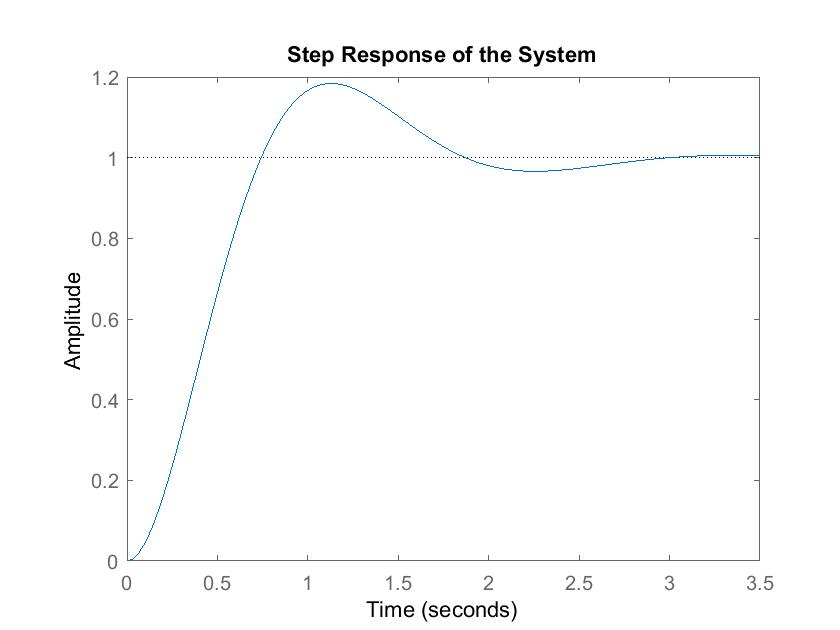
\includegraphics[width=0.5\textwidth]{figs/10.2.jpg}
    \caption{The System Response Over Time.}
    \label{fig:yb}
\end{figure}
\clearpage

\subsection{Lyapunov Stability}

The origin is a singular point for the pair of equations
\[
\frac{dx_1}{dt} = ax_1 + bx_2 \quad \text{and} \quad \frac{dx_2}{dt} = cx_1 + dx_2
\]
Using Lyapunov theory, find sufficient conditions on \(a\), \(b\), \(c\), and \(d\) such that the origin is asymptotically stable.

\textbf{\textcolor{red}{Solution :}} \\
We choose a function
\[ V = x_1^2 + x_2^2 \]
which is positive for all \(x_1\), \(x_2\) except \(x_1 = x_2 = 0\). The time derivative of \(V\) is
\[
\frac{dV}{dt} = 2x_1 \frac{dx_1}{dt} + 2x_2 \frac{dx_2}{dt} = 2ax_1^2 + 2bx_1x_2 + 2cx_1x_2 + 2dx_2^2
\]
To make \(\frac{dV}{dt}\) negative for all \(x_1\), \(x_2\), we might choose \(a < 0\), \(d < 0\), and \(b = -c\). In this case,
\[
\frac{dV}{dt} = 2ax_1^2 + 2dx_2^2 < 0
\]
except when \(x_1 = x_2 = 0\). Hence one set of sufficient conditions for asymptotic stability are \(a < 0\), \(d < 0\), and \(b = -c\). There are other possible solutions to this problem.
\clearpage

\subsection{Lyapunov Stability}

Determine sufficient conditions for the stability of the origin of the nonlinear discrete-time system described by
\[ x_1(k+1) = x_1(k) - f[x_1(k)] \]
\textbf{\textcolor{red}{Solution :}} \\
Let \(V[x(k)] = [x_1(k)]^2\), which is greater than \(0\) for all \(x \neq 0\). Then, 
\begin{align}
    \Delta V &= x_1^2(k+1) - x_1^2(k) = (x_1(k)-f[x_1(k)])^2 -x_1^2(k) \\
        & = x_1(k)f[x_1(k)]\left( \frac{f[x_1(k)]}{x_1}-2\right)
\end{align}

Therefore sufficient conditions for \(\Delta V \leq 0\) and thus stability of the system are
\[ x_1f(x_1) \geq 0 \]
and
\[ \frac{f(x_1)}{x_1} \leq 2 \quad \text{for all} \quad x_1\]
\clearpage

\subsection{Lyapunov Stability}

Determine sufficient conditions for the global stability of the system. 
\begin{equation}
    \dot{x} = Ax + bf(x_1) \quad \text{where} \quad A = \begin{bmatrix}
        -2 & -1 \\ 0 & -2
    \end{bmatrix}, \quad b = \begin{bmatrix}
        1 \\ 2
    \end{bmatrix}
\end{equation}

\textbf{\textcolor{red}{Solution :}} \\
Let \(V = x^T P x\) and \(P = \begin{bmatrix} a & c \\ c & 1 \end{bmatrix}\). Then,
\begin{align}
    \dot{V} &= x^T(PA + A^T P)x + x^T P b f(x_1) + f(x_1) b^T P x \\
    & = x^T \begin{bmatrix}
        -4a & -a-4c \\ -a-4c & -2c-4
    \end{bmatrix}x + 2(a+2c)x_1f(x_1) + 2(c+2)x_2f(x_1)
\end{align}  
To eliminate the cross-product term \(x_2 f(x_1)\), set \(c = -2\). Then,
\[ \dot{V} = -x^T Q x + 2(a-4)x_1 f(x_1) \]
Where \(Q = \begin{bmatrix}
    4a & a-8 \\ a-8 & 0
\end{bmatrix}\). For \(Q \geq 0\), \(a = 8\). The resulting \(\dot{V}\) is
\begin{equation}
    \dot{V} = -32 x_1^2 + 8x_1f(x_1) = -8x_1^2\left(4 - \frac{f(x_1)}{x_1}\right)
\end{equation}
Then \(\dot{V} \leq 0\) and the system is stable if \(\frac{f(x_1)}{x_1} \leq 4\) for all \(x_1 \neq 0\).
\clearpage

\subsection{Linearization}

Consider the following nonlinear system:
$$\dot{x}(t) = f(x,u) =  -4x(t) - 2u(t) + u(t)^3.$$
\begin{itemize}
    \item[(a)] Find an equilibrium $(\bar{x},\bar{u})$ with $\bar{u} = 2.$
    \item[(b)] Linearize the dynamics around $(\bar{x},\bar{u})$. Find the value of $a_0$ and $b_0$ of the linearized model in the form:
    \begin{align*}
        &\dot{\delta}_x(t) + a_0 \delta_x(t) = b_0 \delta_u(t), \\
        &\text{where}\,\, \delta_x(t) := x(t) - \bar{x} \,\, \text{and} \,\, \delta_u(t) := u(t) - \bar{u}.
    \end{align*}
        \end{itemize}
\textbf{\textcolor{red}{Solution :}} \\
\begin{itemize}
    \item[(a)] $\bar{x} = 1.$ \\
    Steps:
    Solve $-4\bar{x} - 2\bar{u} + \bar{u}^3 = 0$ with $\bar{u} = 2$ gives $\bar{x} = 1$.  
    \item[(b)] $(a_0, b_0) = (4, 10).$ \\
    Steps:
    $\delta_x = x - \bar{x} = x-1$, $\delta_u = u - \bar{u} = u -2$. Then we have
    \begin{equation*}
        \dot{\delta}_x(t) \approx f(\bar{x}, \bar{u}) + \frac{\partial f}{\partial x} (\bar{x}, \bar{u}) \delta_x + \frac{\partial f}{\partial u} (\bar{x}, \bar{u}) \delta_u = -4 \delta_x + 10 \delta_u.
        \end{equation*}
\end{itemize}

\clearpage
\subsection{Controllability}

Consider the following system:
$$\dot{x} =\bmat{1 & 0 \\ 0 &-2}x + \bmat{1 \\ b} u \qquad y=\bmat{1 & 1}x$$
What value of $b$ leads to the loss of controllability in the system? \\
\textbf{\textcolor{red}{Solution :}} \\
System's transfer function is given by:
$$G(s) = C(sI - A)^{-1}B= \frac{s + 2 + b(s - 1)}{(s+2)(s-1)}$$
We can see that setting $b=0$ leads to pole-zero cancellation and loss of controllability in the system. Alternatively, it can also be checked by:
$$\mathcal{C}(A,B)=\pmat{1 & 1\\ b & -2b}$$
and for $b = 0$, rank$(\mathcal{C}(A, B)) = 1 <2$.
\clearpage

\section{System Sensitivity Measures}
\subsection{Sensitivity Transfer Function}

The closed-loop should have zero steady-state error for step reference commands. 

\begin{itemize}
    \item[(a)] What is the the value of the sensitivity transfer function $S(s)$ at $s= 0$?
    \item[(b)] What is the the value of the loop transfer function $|L(0)|$ at $s= 0$?
    \end{itemize}

\textbf{\textcolor{red}{Solution :}} \\
\begin{itemize}
    \item[(a)] $S(0) = 0$.  \\
    Since the closed-loop system have zero steady-state error: $e(t) \to 0$ as $t \to \infty$. We must have $S(0) = 0$. 
    \item[(b)] $|L(0)| = +\infty$.  \\
    Since $S(s) = \dfrac{1}{1+L(s)}$, $S(0) = 0$ implies that $|L(0)| = +\infty$.  
\end{itemize}

\clearpage
\subsection{Sensitivity Transfer Function}

The closed-loop should have an error $e(t) \le 0.1$ for reference commands $r(t) = 2 \sin(\omega t)$  with $\omega \le 10 \,\text{rad}/\sec$. This means that $|S(j\omega)|\le A$ for $\omega \le B\,\text{rad}/\sec$. What is the value of $A$ and $B$?
\textbf{\textcolor{red}{Solution :}} \\
$(A,B) = (0.05, 10)$. \\
Steps: \\
We have $e(t) = 2 |S(j\omega)| \sin(\omega t + \measuredangle S(j\omega))$. \\
Since $e(t) \le 0.1$ for $\omega \le 10 \,\text{rad}/\sec$, we must have:
$$|S(j\omega)| \le \frac{0.1}{2} = 0.05$$
for $\omega \le 10 \,\text{rad}/\sec$. 
\clearpage

\subsection{Closed-Loop Transfer Function}

The closed-loop should have an output $y(t) \le 0.05$ for reference commands $n(t) = 10 \sin(\omega t)$  with $\omega \ge 1000 \,\text{rad}/\sec$. This means that $|T(j\omega)|\le A$ for $\omega \ge B\,\text{rad}/\sec$. What is the value of $A$ and $B$?



\textbf{\textcolor{red}{Solution :}} \\
$(A,B) = (0.005, 1000)$. \\
Steps: \\
We have $y(t) = -10 |T(j\omega)| \sin(\omega t + \measuredangle T(j\omega))$. \\
Since $y(t) \le 0.1$ for $\omega \ge 1000 \,\text{rad}/\sec$, we must have:
$$|T(j\omega)| \le \frac{0.05}{10} = 0.005$$
for $\omega \ge 1000 \,\text{rad}/\sec$. 
\clearpage

\section{Loop-Shaping}
\subsection{Loop Gain}

We plan to design a controller $K(s)$ for a system with transfer function given by $G(s)$. The controller and the system are in standard unity feedback setting. Let $e=r-y$ where $r$ and $y$ representing the reference and the output signals respectively. Let $n$ represent the output noise i.e. if $n \neq 0$ then $e=r- (y+n)$. The specifications are to design a controller so that the closed loop is stable and has:
\begin{itemize}
    \item [(a)] gain less than 0.01 from reference r to error e for frequencies below 0.1 rad/sec.
    \item [(b)] gain less than 0.04 from input n to output y for frequencies above 200 rad/sec. 
\end{itemize}
Translate the above specifications into requirements on the loop gain $|L(j \omega)|$ where loop gain is given by $L(s)=K(s) G(s)$.\\

\textbf{\textcolor{red}{Solution :}} \\
The transfer function from $r$ to $e$ is $S(s) =\frac{1}{1 + L(s)}$. The steady error due to a
unit step reference input $r(t) = \bar{r}$ is given by $e = S(0) \bar{r}$. Thus specification (a) is equivalent to $|S(j\omega)| \leq 0.01$ for $\omega \leq 0.1 \frac{rad}{sec}$. This is approximately equivalent to $|L(j\omega)| \geq 99$ for $\omega \leq 0.1 \frac{rad}{sec}$.

The transfer function from $n$ to $y$ is $-T(s) =\frac{-L(s)}{1+L(s)}$. Specification (b) corresponds to $|T(j\omega)| \leq 0.04$ for $\omega \geq 200 \frac{rad}{sec}$ and this is approximately equivalent to $|L(j\omega)| \leq 0.04$ for $\omega \geq 200 \frac{rad}{sec}$.
\clearpage

\subsection{Proportional Controller}

A model for a DC motor is:
$$J \dot{y} + by = c V $$
where $y$ is the angular velocity of the motor shaft (deg/sec), and V is the input voltage (Volts).
The model parameters are: $J=3$ N m sec2/deg2 , $b=5$ Nm sec/deg, and gain from input voltage to applied torque $c=12$ Nm/Volts. We plan to design a controller $K(s)$ for this system. The controller and the system are in standard unity feedback setting. Let $e=r-y$ where $r$ is the reference signal. Let $n$ represent the output noise i.e. if $n \neq 0$ then $e=r-(y+n)$. Design a a proportional control law $K(s) = K_p$ so that the closed loop is stable and has gain less than 0.01 from reference $r$ to error $e$ for frequencies below 0.1 rad/sec.
    
\textbf{\textcolor{red}{Solution :}} \\
Firstly, we can show that the requirement of gain less than 0.01 from reference $r$ to error $e$ for frequencies below 0.1 rad/sec translates to $|L(j \omega)|=|K(j \omega) G(j \omega)| \geq 100$ for $\omega \leq 0.1 \frac{rad}{sec}$. The system transfer function is $G(s) =\frac{12}{3s + 5}$. This has a corner frequency at  $\omega=1.6$ rad/sec and DC gain $G(0) = 2.4$. Thus $K_p =\frac{100}{2.4}$ will ensure the gain requirement is approximately satisfied. Additionally, we can verify the closed loop pole of the system with $K_p =\frac{100}{2.4}$ is in the LHP so the closed loop system is stable. Thus both the requirements are met.  
\clearpage

\subsection{Proportional Controller}

We plan to design a controller $K(s) = K_p$ for a system with transfer function $G(s)$ given by:
\[
G(s) = \frac{12}{3s + 5}
\]
The controller and the system are in standard unity feedback setting. Let $e=r-y$ where $r$ and $y$ representing the reference and the output signals respectively. Let $n$ represent the output noise i.e. if $n \neq 0$ then $e=r- (y+n)$. The specification is to design a controller so that the closed loop is stable and has gain less than 0.04 from input n to output y for frequencies above 200 rad/sec. What is the cross-over frequency. 
 
\textbf{\textcolor{red}{Solution :}} \\
Firstly, we can show that the requirement of gain less than 0.04 from input $n$ to output $y$ for frequencies greater then 200 rad/sec translates to $|L(j \omega)|=|K(j \omega) G(j \omega)| \leq 0.04$ for $\omega \geq 200 \frac{rad}{sec}$. Thus $K_p \leq \frac{0.04}{|G(j200)|} \approx 2$ will ensure this requirement. Additionally, we can verify the closed loop pole of the system with $\frac{-5}{12}<K_p$ is in the LHP so the closed loop system is stable. Thus choosing \(K_p = 2\) meet the both requirements.  

The cross-over frequency is approximately 7.82 rad/sec.\\
\clearpage

\subsection{Design a Stable Controller}

Given a system's transfer function $G(s) =\frac{12}{3s + 5} $, use loop-shaping procedure to design a controller $K(s)$ such that the closed loop system is stable and it satisfies:
\begin{itemize}
    \item [(a)] has a loop crossover frequency near 20 rad/sec.
    \item [(b)] gain less than 0.01 from reference r to error e for frequencies below 0.1 rad/sec.
    \item [(c)] gain less than 0.04 from input n to output y for frequencies above 200 rad/sec. 
\end{itemize}
Verify that the closed-loop is stable with your control design.

\textbf{\textcolor{red}{Solution :}} \\
We can use a proportional gain to set the loop cross-over frequency (requirement (a)). Then use an integral boost and roll-off to satisfy requirements (b) and (c) respectively. This may require some iteration to get values that meet all design specifications.

First we choose the proportional gain so that the loop gain has crossover $|L(j\omega_c)| =|K(j \omega_c) G(j \omega_c)| = 1$ at $\omega_c = 20$ rad/sec. This can be done with the gain $K_1 = \frac{1}{|G(j\omega_c)|} \approx 5.02$. This will give the first loop-shape $L_1(s) = G(s)K_1$. The first loop shape has DC gain $L_1(s) = K_1 G(s)$. Thus we need to increase the gain by a factor of $\frac{100}{12} = 8.4$ to ensure that we satisfy requirement (b). We'll use an integral boost 
$K_2(s) =\frac{s+\bar{\omega}_2}{s}$ where $\bar{\omega}_2$ is the frequency below which the gain starts to increase. With some iteration the choice $\bar{\omega}_2=5$rad/sec seem to easily exceed the low frequency requirement. Notice that $\bar{\omega}_2 < \omega_c$. For stability and robustness reasons we need the slope
of $|L|$ to be shallow near $\omega_c$. Thus we need to choose our low-frequency boost to start
sufficiently below $\omega_c$ that it doesn't have a significant impact on the slope at $\omega_c$. After
this stage our controller is $K_1 K_2(s)$ and our loop-shape is $L_2(s) = K_1 K_2(s)G(s)$.
Finally, we need to modify the loop shape to satisfy the design requirement iv. We can
choose a roll-off to decrease the high frequency gain $K_3(s) =\frac{\bar{\omega}_3}{s+\bar{\omega}_3}$. Again, we want to choose $\bar{\omega}_3 > \omega_c$ so that the roll-off has negligible effect on the slope of $|L|$ near cross-over. However, we also want to choose $\bar{\omega}_3$ small enough that we decrease the high frequency gain enough to satisfy $|L(j200)| \leq  0.0385$. After some trial and error $\bar{\omega}_3= 80$ rad/sec ensures that the requirements are satisfied. Our final controller is
$K(s) = K_1K_2(s)K_3(s)$ and our final loop-shape is $L_2(s) = K(s)G(s)$. The Bode plot and step responses are shown below. The step response has a small steady state error and good noise rejection. The response also has a small overshoot.

\begin{figure}[H]
    \centering
    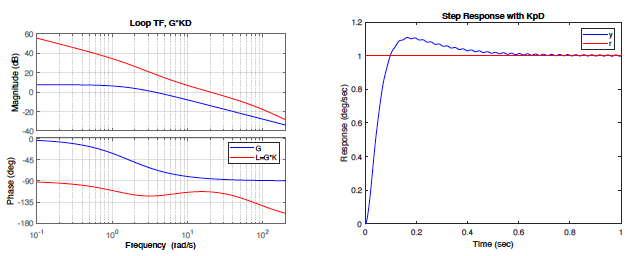
\includegraphics[width=\linewidth]{figs/12.4.png}
    \caption{Bode Plot and Step Response for Closed Loop System }
    \label{fig:enter-label}
\end{figure}

\clearpage























































\end{document}


